%*********************************************************************
% fduthesis: 复旦大学论文模板
% 2020/08/30 v0.7e
%
% 重要提示:
%   1. 请确保使用 UTF-8 编码保存
%   2. 请使用 XeLaTeX 或 LuaLaTeX 编译
%   3. 请仔细阅读用户文档
%   4. 修改、使用、发布本文档请务必遵循 LaTeX Project Public License
%   5. 不需要的注释可以尽情删除
%*********************************************************************

\documentclass[type=master, oneside, draft=false]{fduthesis}
% 模板选项:
%   type = doctor|master|bachelor  论文类型,默认为本科论文
%   oneside|twoside                论文的单双面模式,默认为 twoside
%   draft = true|false             是否开启草稿模式,默认关闭
% 带选项的用法示例:
%   \documentclass[oneside]{fduthesis}
%   \documentclass[twoside, draft=true]{fduthesis}
%   \documentclass[type=bachelor, twoside, draft=true]{fduthesis}

% 页眉:左标题右章节
% \makeatletter
% \let\ps@plain\ps@fancy
% \makeatother
% \fancyhf{}
% \fancyhead[L]{\small\nouppercase{基于多源知识的安全漏洞影响组件的识别方法}}
% \fancyhead[R]{\small\nouppercase{\csname l__fdu_header_center_mark_tl\endcsname\leftmark}}
% \fancyfoot[C]{\small\thepage}
% \pagestyle{fancy}

% 魔改模板:根据学院要求改的格式
\makeatletter
\ExplSyntaxOn
% 专业:改为“专业学位类别(领域)”
% \tl_set:Nn \c__fdu_name_major_tl { 专业学位类别(领域) }
\__fdu_patch_cmd:Nnn \__fdu_cover_info: { 6em } { 9em }
% 页眉:左论文标题、右章节名
\let\ps@plain\ps@fancy
\fancyhf{}
\fancyhead[L]{\small\nouppercase{\fdu@kai\l__fdu_info_title_tl}}
\fancyhead[R]{\small\nouppercase{\fdu@kai\l__fdu_header_center_mark_tl\leftmark}}
\fancyfoot[C]{\small\thepage}
\pagestyle{fancy}
% 摘要:用逗号而不是封号分隔关键词
% \cs_set_protected:Npn \__fdu_abstract_end:
% {
%   \__fdu_keywords:nNn
%   { \sffamily \c__fdu_name_keywords_tl \c__fdu_fwid_colon_tl }
%   \l__fdu_info_keywords_clist { \c__fdu_fwid_comma_tl }
%   \__fdu_clc:nn
%   { \sffamily \c__fdu_name_clc_tl \c__fdu_fwid_colon_tl }
%   { \l__fdu_info_clc_tl }
% }
% \cs_set_protected:Npn \__fdu_abstract_en_end:
% {
%   \__fdu_keywords:nNn
%   { \bfseries \c__fdu_name_keywords_en_tl \__fdu_quad: }
%   \l__fdu_info_keywords_en_clist { , ~ }
%   \__fdu_clc:nn
%   { \bfseries \c__fdu_name_clc_en_tl \__fdu_quad: } 
%   { \l__fdu_info_clc_tl } 
% }
% 摘要:页数从罗马小写改为大写
\ctex_patch_cmd:Nnn \frontmatter
  { roman } { Roman }
\ExplSyntaxOff
\makeatother

\fdusetup{
  % 参数设置
  % 允许采用两种方式设置选项:
  %   1. style/... = ...
  %   2. style = { ... = ... }
  % 注意事项:
  %   1. 不要出现空行
  %   2. “=” 两侧的空格会被忽略
  %   3. “/” 两侧的空格不会被忽略
  %   4. 请使用英文逗号 “,” 分隔选项
  %
  % style 类用于设置论文格式
  style = {
    font = times,
    % 西文字体(包括数学字体)
    % 允许选项:
    %   font = garamond|libertinus|lm|palatino|times|times*|none
    %
    cjk-font = windows,
    % 中文字体
    % 允许选项:
    %   cjk-font = adobe|fandol|founder|mac|sinotype|sourcehan|windows|none
    %
    % 注意:
    %   1. 中文字体设置高度依赖于系统。各系统建议方案:
    %        windows:cjk-font = windows
    %        mac:    cjk-font = mac
    %        linux:  cjk-font = fandol(默认值)
    %   2. 除 fandol 和 sourcehan 外,其余字体均为商用字体,请注意版权问题
    %   3. 但 fandol 字体缺字比较严重,而 sourcehan 没有配备楷体和仿宋体
    %   4. 这里中西文字体设置均注释掉了,即使用默认设置:
    %        font     = times
    %        cjk-font = fandol
    %   5. 使用 font = none / cjk-font = none 关闭默认字体设置,需手动进行配置
    %
    font-size = -4,
    % 字号
    % 允许选项:
    %   font-size = -4|5
    %
    % fullwidth-stop = catcode,
    % 是否把全角实心句点 “.” 作为默认的句号形状
    % 允许选项:
    %   fullwidth-stop = catcode|mapping|false
    % 说明:
    %   catcode   显式的 “。” 会被替换为 “.”(e.g. 不包括用宏定义保存的 “。”)
    %   mapping   所有的 “。” 会被替换为 “.”(使用 LuaLaTeX 编译则无效)
    %   false     不进行替换
    %
    footnote-style = xits,
    % 脚注编号样式
    % 允许选项:
    %   footnote-style = plain|libertinus|libertinus*|libertinus-sans|
    %                    pifont|pifont*|pifont-sans|pifont-sans*|
    %                    xits|xits-sans|xits-sans*
    %
    hyperlink = none,
    % 超链接样式
    % 允许选项:
    %   hyperlink = border|color|none
    %
    % hyperlink-color = default,
    % 超链接颜色
    % 允许选项:
    %   hyperlink-color = default|classic|elegant|fantasy|material|
    %                     business|science|summer|autumn|graylevel|prl
    % 默认与西文字体保持一致
    %
    bib-backend = bibtex,
    % 参考文献支持方式
    % 允许选项:
    %   bib-backend = bibtex|biblatex
    %
    % bib-style = numerical,
    % 直接TMD改模板好了:D:\texlive\2021\texmf-dist\bibtex\bst\gbt7714\gbt7714-numerical.bst
    % Ban: address, publisher, doi, 非 EB/OL 的 url
    % 参考文献样式
    % 允许选项:
    %   bib-style = author-year|numerical|<其他样式>
    % 说明:
    %   author-year  著者—出版年制
    %   numerical    顺序编码制
    %   <其他样式>   使用其他 .bst(bibtex)或 .bbx(biblatex)格式文件
    %
    % cite-style = {},
    % 引用样式
    % 默认为空,即与参考文献样式保持一致
    % 仅适用于 biblatex;如要填写,需保证相应的 .cbx 格式文件能被调用
    %
    bib-resource = {src/ref.bib},
    % 参考文献数据源
    % 可以是单个文件,也可以是用英文逗号 “,” 隔开的一组文件
    % 如果使用 biblatex,则必须明确给出 .bib 后缀名
    %
    % logo = {fudan-name.pdf},
    % 封面中的校名图片
    % 模版已自带,通常不需要额外配置
    %
    % logo-size = {0.5\textwidth},      % 只设置宽度
    % logo-size = {{}, 3cm},            % 只设置高度
    % logo-size = {8cm, 3cm},           % 设置宽度和高度
    % 设置校名图片的大小
    % 通常不需要调整
    %
    auto-make-cover = false % 盲审要求
    % 是否自动生成论文封面(封一)、指导小组成员名单(封二)和声明页(封三)
    % 除非特殊需要(e.g. 不要封面),否则不建议设为 false
  },
  %
  % info 类用于录入论文信息
  info = {
    title = {基于多源知识的开源软件漏洞的补丁识别方法},
    % 中文标题
    % 长标题建议使用 “\\” 命令手动换行(不是指在源文件里输入回车符,当然
    % 源文件里适当的换行可以有助于代码清晰):
    %   title = {最高人民法院、最高人民检察院关于适用\\
    %            犯罪嫌疑人、被告人逃匿、死亡案件违法所得\\
    %            没收程序若干问题的规定},
    %
    title* = {Finding Patches for Open Source Software Vulnerabiliies from Multi-Source Knowledge},
    % 英文标题
    %
    author = {许聪颖},
    % author = {},  % 盲审要求
    % 作者姓名
    %
    % author* = {Your name},
    % 作者姓名(英文 / 拼音)
    % 目前不需要填写
    %
    supervisor = {陈碧欢\quad 副教授},
    % supervisor = {},  % 盲审要求
    % 导师
    % 姓名与职称之间可以用 \quad 打印一个空格
    %
    major = {软件工程},
    % 专业
    %
    degree = academic,
    % 学位类型
    % 允许选项:
    %   degree = academic|professional
    % 说明:
    %   academic      学术学位
    %   professional  专业学位
    %
    department = {软件学院},
    % 院系
    %
    student-id = {19212010035},
    % student-id = {},  % 盲审要求
    % 作者学号
    %
    % date = {2020 年 1 月 1 日},
    % 日期
    % 注释掉表示使用编译日期
    %
    % secret-level = ii,
    % 密级
    % 允许选项:
    %   secret-level = none|i|ii|iii
    % 说明:
    %   none  不显示密级与保密年限
    %   i     秘密
    %   ii    机密
    %   iii   绝密
    %
    % secret-year = {五年},
    % 保密年限
    % secret-level = none 时该选项无效
    %
    instructors = {
      {赵文耘 \quad 教\quad 授},
      {彭\quad 鑫 \quad 教\quad 授},
      {陈碧欢     \quad 副教授},
      {沈立炜     \quad 副教授}
    },
    % instructors = {}, % 盲审要求
    % 指导小组成员
    % 使用英文逗号 “,” 分隔
    % 如有需要,可以用 \quad 手工对齐
    %
    keywords = {开源软件,漏洞,补丁},
    % 中文关键字
    % 使用英文逗号 “,” 分隔
    %
    keywords* = {Open Source Software, Vulnerabilities, Patches},
    % 英文关键字
    % 使用英文逗号 “,” 分隔
    %
    clc = {TP311}
    % 中图分类号
  }
}

% 需要的宏包可以自行调用
% \usepackage{amsthm}
\usepackage{amsmath,bm}
% \theoremstyle{acmdefinition}
\newtheorem{exmp}{Example} %这个地方贼麻烦,解决了老半天
\usepackage{booktabs}
\usepackage[labelsep=quad]{caption}
\usepackage{diagbox}
\usepackage{enumerate}
\usepackage{enumitem}
\usepackage{listings}
\usepackage{makecell}
\usepackage{physics}
\usepackage{threeparttable}
\usepackage{xcolor}
\usepackage{xspace}
\usepackage{tcolorbox}
\usepackage{stfloats}
\usepackage{subcaption}
\usepackage{graphicx}
\usepackage{multirow}
\usepackage{url}




\setenumerate[1]{itemsep=0pt,partopsep=0pt,parsep=\parskip,topsep=5pt}
\setitemize[1]{itemsep=0pt,partopsep=0pt,parsep=\parskip,topsep=5pt}
\setdescription{itemsep=0pt,partopsep=0pt,parsep=\parskip,topsep=5pt}
\ctexset{subsection/tocline={\CTEXnumberline{#1}#2}}

\lstset{
  % basicstyle=\small\tt,
  basicstyle=\normalfont\ttfamily,
  numbers=left,
  % numberstyle=\small\tt,
  numberstyle=\normalfont\ttfamily\color{darkgray},
  stepnumber=1,
  numbersep=8pt,
  frame=single,
  xleftmargin=3em,
  xrightmargin=1em,
  framexleftmargin=2em,
  captionpos=b,
  keywordstyle=\color{blue!70}, commentstyle=\color{red!50!green!50!blue!50},
  rulesepcolor=\color{red!20!green!20!blue!20},
}
\lstdefinelanguage{json}{
  literate=
    {\{}{{{\color{blue}{\{}}}}{1}
    {\}}{{{\color{blue}{\}}}}}{1}
    {[}{{{\color{blue}{[}}}}{1}
    {]}{{{\color{blue}{]}}}}{1},
}

% 需要的命令可以自行定义
\newcommand{\hilbertH}{\symcal{H}}
\newcommand{\ee}{\symrm{e}}
\newcommand{\ii}{\symrm{i}}
\newcommand{\ds}{\,\cdot\,}

\newcolumntype{C}[1]{>{\centering\arraybackslash}m{#1}}

\makeatletter
\newcommand\footnoteref[1]{\protected@xdef\@thefnmark{\ref{#1}}\@footnotemark}
\makeatother


\includeonly{
  src/a1_abstract.tex, src/a2_abstract_en.tex,
  src/c1_introduction.tex, src/c2_background.tex, src/c3_empirical.tex,
  src/c4_approach.tex, src/c5_experiment.tex, src/c6_related.tex, src/c7_summary.tex,
  src/z1_acknowledgement.tex, src/z2_review.tex
}

\begin{document}
% 盲审要求:指导小组成员不要了,独创性声明不要了
\begin{titlepage}
  \makecoveri     % 封面
  \newpage
  % \makecoverii    % 指导小组
\end{titlepage}

\renewcommand{\captionfont}{\small}
\renewcommand{\lstlistingname}{代码}
\renewcommand{\lstlistlistingname}{代码}
\renewcommand{\thelstlisting}{\thechapter-\arabic{lstlisting}}

\newcommand{\congyingEdit}[1]{\textcolor{black}{#1}}
\newcommand{\tocheck}[1]{\textcolor{black}{#1}}
\newcommand{\tool}{\textsc{Tracer}\xspace}
\newcommand{\fn}[1]{\footnote{\scalebox{0.82}{#1}}}

% 这个命令用来关闭版心底部强制对齐,可以减少不必要的 underfull \vbox 提示,但会影响排版效果
% \raggedbottom

% 前置部分包含目录、中英文摘要以及符号表等
\frontmatter

\tableofcontents                  % 目录
% !TeX root = ../main.tex
\begin{abstract}

开源软件(Open Source Software, OSS)漏洞管理已成为一个备受关注的研究问题。开源软件漏洞数据库作为各项软件安全任务的基础设施,数据库中漏洞知识的质量受到了越来越多的关注和研究。然而,现有的漏洞数据库中补丁知识的质量和特征尚未被系统地研究。此外,漏洞数据库中的补丁也多是由人工或基于启发式规则的方法半自动化收集。这些方法人工成本高并且为任务定制化,无法应用于所有开源软件漏洞。

针对上述问题,本文先开展了一项针对开源软件漏洞补丁的经验研究,以了解当前商业漏洞数据库中开源软件漏洞补丁的质量和特征。该经验研究涵盖五个方面,包括补丁覆盖度分析、补丁一致性分析、补丁类型分析、补丁映射关系以及补丁准确性分析。研究发现:(1)商业漏洞数据库中开源软件漏洞补丁的质量并不理想。补丁缺失情况较为普遍,商业数据库中漏洞的补丁覆盖率仅为41.0\%左右。对于有多个补丁的漏洞,商业数据库经常会遗漏一些补丁。(2)开源软件漏洞补丁在类型、映射关系方面有一定的特殊性。93.7\%的补丁类型都是GitHub的代码提交,超过40\%的漏洞与其补丁是一对多的映射关系。

基于经验研究的发现,本文提出了一种名为\tool 的基于多源知识的开源软件漏洞的补丁识别方法。该方法用于识别代码提交类型的补丁,并构建一对多的漏洞补丁映射关系。该方法的核心思想是:漏洞的补丁会在与该漏洞相关的各种来源的漏洞公告、分析报告、讨论和解决的过程中被频繁地提及和引用。因此,本文首先设计了一种基于多知识源的漏洞参考链接网络,再从该网络中选出具有最高置信度和连通度的补丁节点作为结果,并基于选定的补丁进行补丁扩增,从而构建一对多的漏洞补丁映射关系。

本文通过五个研究问题,从准确性、通用性、实用性等多个方面对\tool 进行了实验评估。实验结果表明:(1)在包含1,295个漏洞的实验数据集上,\tool 可以达到88.0\%的补丁覆盖率、0.864的精确率和0.864的召回率。(2)与现有的基于启发式规则的方法相比,\tool 将补丁覆盖率提高\tocheck{58.6\%}到\tocheck{273.8\%},将F1值提高\tocheck{116.8\%}。(3)与商业漏洞数据库$DB_A$和$DB_B$相比,\tool 的召回率高出18.4\%。这表明,\tool 可用于补充现有漏洞数据库缺失的漏洞补丁数据。(4)在更大范围的开源软件漏洞上,\tool 具有较好的通用性。即使在商业漏洞数据库$DB_A$和$DB_B$都没有补丁的情况下,\tool 仍可以找到大量漏洞的补丁。这表明,\tool 可以极大地补充或增强现有的商业漏洞数据库。在实际工作场景中,\tool 有助于用户更准确、更快速地识别到补丁。
\end{abstract}
     % 摘要
% !TeX root = ../main.tex
\begin{abstract*}
Open source software (OSS) vulnerability management has become an open problem. Vulnerability databases is valuable by providing valuable data that is needed to address OSS vulnerabilities. As a result, there also arises a growing concern about the information quality of vulnerability databases. However, it is unclear how the quality and features of patches in existing vulnerability databases are. Further, existing manual or heuristic-based approaches for patch identification are either too expensive or too specific to be applied to all OSS vulnerabilities.

To address these problems, we first conduct an empirical study to understand the quality and characteristics of patches for OSS vulnerabilities in two state-of-the-art vulnerability databases. Our study is designed to cover five dimensions, i.e., the coverage, consistency, type, cardinality and accuracy of patches. Then, inspired by our study, we propose an automated approach, named \tool, to find patches for an OSS vulnerability from multiple sources, by constructing a reference network. %Our key idea is that patch commits will be frequently referenced during the reporting, discussion and resolution of an OSS vulnerability.

The extensive evaluation has indicated that (1) \tool finds patches for up to 273.8\% more CVEs than existing heuristic-based approaches while achieving a significantly higher F1-score by up to 116.8\%; (2) \tool achieves a higher recall by up to 18.4\% than state-of-the-art vulnerability databases, but sacrifices up to 12.0\% fewer CVEs (whose patches are not found) and 6.4\% lower precision; (3) \tool is general to all OSS vulnerabilities and useful in practice.

% Our evaluation has also demonstrated the generality and usefulness of \tool.
\end{abstract*}  % 英文摘要

% 主体部分是论文的核心
\mainmatter

\chapter{绪论}

% 本章节概述了背景、研究目的与意义\cite{jia2021:oss-vulnerability, mitre2021:cve}。
本章将阐述本文的研究背景、研究问题、主要工作、主要贡献以及本文的篇章结构。

\section{研究背景}

开源软件(Open Source Software,OSS)为开源及闭源应用程序的开发提供了基础。得益于开源社区的蓬勃发展,在软件开发过程中,开发人员经常会使用开源软件中已实现的功能,节省开发时间,加快开发速度\cite{Wang2020empirical}。然而,伴随着开发效率的提高,开源软件中的安全漏洞也会被引入软件系统中\cite{2何熙巽2020软件供应链安全综述,3刘剑2018软件与网络安全研究综述}。据Synopsys公司发布的《开源安全和风险分析报告》\footnote{https://www.synopsys.com/content/dam/synopsys/sig-assets/reports/rep-ossra-2021.pdf}显示,在所分析的1,500个应用程序中,98\%的应用程序都使用了开源软件。
%然而,大规模使用开源软件可以加速应用程序开发的进程,但同时也引入了安全风险。
报告指出,有84\%的应用程序包含至少一个已知的开源软件漏洞,对比于前一年(2019年),增加了9\%。此外,据Snyk公司发布的报告\footnote{https://snyk.io/wp-content/uploads/sooss\_report\_v2.pdf}显示,近些年,开源软件中所披露的漏洞越来越多,过去两年间几乎翻了一倍。

针对上述问题,已有大量工作研究如何降低开源软件漏洞所带来的安全风险,包括通过学习漏洞特征来检测开源软件中的漏洞\cite{li2016vulpecker,li2018vuldeepecker,zhou2019devign,jimenez2019importance}、通过匹配漏洞及补丁签名\cite{jang2012redebug, kim2017vuddy, xu2020patch, xiao2020mvp, cui2020vuldetector}修复开源软件中的漏洞\cite{mulliner2013patchdroid, duan2019automating, xu2020automatic, machiry2020spider}、进行软件成分分析以确定应用程序中的开源软件漏洞是否在执行路径上\cite{pashchenko2018vulnerable, ponta2020detection, pashchenko2020vuln4real, Wang2020empirical}。在这些工作中,完整且准确的漏洞数据十分重要,例如,漏洞描述、受漏洞影响的软件、版本以及补丁等知识都是这些工作得以开展的基础。目前,已有多方人员致力于构建安全漏洞数据库。在安全社区中,由美国政府资助的CVE List\footnote{https://cve.mitre.org/cve/}(Common Vulnerabilities \& Exposures)、NVD\footnote{https://nvd.nist.gov}(National Vulnerability Database)和由中国政府资助的CNVD\footnote{https://www.cnvd.org.cn/}(国家信息安全漏洞共享平台)、CNNVD\footnote{http://www.cnnvd.org.cn/}(国家信息安全漏洞数据库)是最具影响力的漏洞数据库,该数据库包含应用软件、系统以及硬件的漏洞。在工业界中,BlackDuck\footnote{https://www.synopsys.com/content/dam/synopsys/sig-assets/datasheets/bdknowledgebase-ds-ul.pdf}、WhiteSource\footnote{https://www.whitesourcesoftware.com/vulnerability-database/}、Veracode\footnote{https://sca.veracode.com/vulnerability-database/search}和Snyk\footnote{https://snyk.io/vuln}等公司较为关注开源软件中的安全漏洞,并已经构建各自的商业数据库。在学术界中,已有很多工作致力于构建漏洞数据集\cite{ponta2019manually,fan2020ac,jimenez2018enabling,gkortzis2018vulinoss,namrud2019androvul},但这些数据集大多是针对特定语言的生态系统或针对特定的软件项目而设计的。

\section{研究问题}
% \textbf{研究问题:}
随着构建的漏洞数据库越来越多,数据库中积累的漏洞数据也越来越多,研究人员开始关注数据库中漏洞信息的质量。Dong等人\cite{dong2019towards}发现了漏洞数据库中受漏洞影响的软件版本信息不准确情况,Chaparro等人\cite{chaparro2017detecting}和Mu等人\cite{mu2018understanding}发现了漏洞描述中普遍缺失关键的漏洞重现步骤。这种不完整或不准确的信息使得安全工作人员难以及时地识别、重现和修复应用程序中的漏洞。

漏洞补丁作为刻画漏洞特征的重要知识,可应用于多种安全相关的任务,包括补丁生成和热部署\cite{mulliner2013patchdroid,duan2019automating,xu2020automatic}、补丁存在测试\cite{zhang2018precise,jiang2020pdiff,dai2020bscout}、软件成分分析\cite{ponta2020detection,pashchenko2020vuln4real,Wang2020empirical}、漏洞检测\cite{li2016vulpecker,li2018vuldeepecker,jang2012redebug,kim2017vuddy, xiao2020mvp, cui2020vuldetector}等。如果漏洞数据库中的补丁知识缺失或不准确,那么这些应用的准确性将会受到严重的影响。然而,漏洞数据库中的补丁知识尚未被系统地研究和评估,目前尚不清楚现有漏洞数据库中补丁的质量情况。

此外,现有的漏洞补丁识别方法主要有三种:(1)人工手动查找漏洞补丁\cite{xu2020automatic,jiang2020pdiff,dai2020bscout,zhou2017automated,sabetta2018practical,chen2020machine,xiao2020mvp,ponta2020detection,pashchenko2020vuln4real},(2)通过启发式规则识别漏洞补丁,比如在CVE引用信息中查找代码提交\cite{duan2019automating,li2016vulpecker}或是在代码提交历史中搜索CVE标识符(CVE ID)\cite{you2017semfuzz,Wang2020empirical},(3)在特定项目的安全公告中搜索漏洞补丁\cite{mulliner2013patchdroid,jang2012redebug,kim2017vuddy}。以上这些方法的人工成本过高,且针对特定的程序语言或项目无法广泛应用于所有开源软件漏洞。

综上,目前的问题是,漏洞数据库中补丁的特征及质量尚未被系统地研究和评估,并且已有的漏洞补丁采集方法通用性较差且人工成本过高。

\section{本文工作}
为解决上述研究问题,本文先开展了一项针对开源软件漏洞补丁的经验研究,以了解当前商业漏洞数据库中开源软件漏洞补丁的质量和特征。然后,基于经验研究的发现,本文提出了一种名为\tool 的基于多源知识的开源软件漏洞的补丁识别方法。该方法通过构建漏洞的多源参考链接网络来识别补丁。本文还进行了大量实验,从准确性、通用性、实用性等多个方面对\tool 进行了评估。

\subsection{开源软件漏洞补丁的经验研究}
为了了解当前商业漏洞数据库中开源软件漏洞补丁的质量和特征,本文挑选了两个认可度较高的商业漏洞数据库作为研究对象。该经验研究涵盖五个方面,包括商业漏洞数据库中补丁覆盖度分析、补丁一致性分析、补丁类型分析、补丁映射关系以及补丁准确性分析。

本文首先构建了一个广度数据集,该数据集包含10,070个开源软件漏洞。在此数据集上,本文分析两个漏洞数据库中开源软件漏洞补丁的覆盖率和一致性。结果表明:在漏洞补丁覆盖率方面,\tocheck{10,070}个漏洞中只有\tocheck{4,602(5.7\%)}的漏洞在商业漏洞数据库中提供了补丁;在漏洞补丁一致性方面,只有\tocheck{19.7\%}的漏洞在两个商业漏洞数据库中有一致的补丁。%\congyingEdit{可以再写些其他的结果}。

基于广度数据集中含补丁的漏洞数据,本文还通过人工构建了一个深度数据集。该数据集包含1,295个开源软件漏洞,且这些漏洞都有补丁。在此数据集上,本文分析了开源软件漏洞补丁的类型和漏洞补丁的映射关系,并评估了商业数据库中漏洞补丁的准确性。结果表明:在漏洞补丁类型方面,\tocheck{1,265(97.7\%)}漏洞的补丁类型都是GitHub或SVN的代码提交;在漏洞补丁映射关系方面,\tocheck{533(41.1\%)}的漏洞与其补丁有一对多的映射关系;在漏洞补丁准确性方面,两个商业数据库的补丁精确率都高于\tocheck{90\%},但对于一对多映射类型的漏洞,两个商业数据库中补丁的召回率都仅为\tocheck{50\%}左右。

这些结果表明,现有的商业漏洞数据库中缺失了许多漏洞的补丁,尤其是对于有多个补丁的漏洞,补丁缺失现象更为严重。这种信息不完整或不准确的情况,使得安全工作人员难以及时地识别、重现和修复开源软件中的漏洞。同时,这也反映出自动化的补丁识别方法的需求,自动化的方法可以帮助工作人员识别并补全缺失的补丁。

\subsection{开源软件漏洞补丁的识别方法}
基于经验研究的发现,本文提出了一个名为\tool 的基于多源知识的开源软件漏洞的补丁识别方法。该方法从多个知识源(即NVD\footnote{https://nvd.nist.gov}、Debian\footnote{https://security-tracker.debian.org/tracker/}、Red Hat\footnote{https://bugzilla.redhat.com/}以及GitHub\footnote{https://github.com/})构建漏洞的参考链接网络并识别补丁(参考链接,即URL网址)。该方法的核心思想是:漏洞的补丁链接会在与该漏洞相关的各种来源的漏洞公告、分析报告、讨论和解决的过程中被频繁提及和引用。因此,本文首先设计了一种基于多知识源的漏洞参考链接网络,然后再从该网络中选出具有最高置信度和连通度的补丁节点作为结果。

\tool 以漏洞的CVE ID作为输入,经过三个步骤,输出该漏洞的补丁。(1)构建多源信息网络,该步骤的目的是将该CVE在被报告、讨论和解决阶段的参考链接进行建模。\tool 从多个\tocheck{漏洞知识源}(即NVD、Debian、Red Hat和GitHub)中提取与该CVE相关的参考链接信息并构建一个信息网络。(2)选择补丁,\tool 从构建的参考链接网络中选择中具有高连通性和高置信度的补丁节点作为该CVE的补丁。(3)扩增补丁,\tool 通过搜索同一代码库所有分支中的相关提交来扩展补丁集。最终,返回所有选中的及扩展的补丁。

\subsection{实验评估}
本文进行了大量实验,通过五个研究问题,从准确性、通用性、实用性等多个方面对\tool 进行了评估。为了评估\tool 的准确性,本文将\tool 与三种基于启发式规则的方法以及两个商业漏洞数据库进行了比较。结果表明,在包含1,295个漏洞的深度数据集上,(1)与现有的基于启发式规则的方法相比,\tool 能够多找到835(273.8\%)漏洞的补丁;同时,在补丁的准确性上,\tool 的F1数值(F1-Score)也比基于启发式规则的方法高116.8\%;(2)与现有的商业漏洞数据库相比,\tool 的召回率(Recall)高出18.4\%;但仍有155(12.0\%)的漏洞\tool 未能找到补丁,\tool 的精确率(Precision)也低了6.4\%。%;(3)\tool 对于大范围开源软件漏洞具有较好的通用性,在实际使用中,也具有较好的实用性。

此外,为了评估\tool 的通用性,本文还另外构建了两个更大的、包含\tocheck{3,185}和\tocheck{5,468}个漏洞的数据集,并在这两个数据集上运行\tool 。结果表明,\tool 在两个数据集上分别可以找到\tocheck{67.7\%}和\tocheck{51.5\%}个漏洞的补丁;精确率分别为\tocheck{0.823}和\tocheck{0.888},召回率分别为\tocheck{0.845}和\tocheck{0.899},这表明\tool 在查找补丁方面具有较好的通用性。

此外,为了评估\tool 的实用性,本文还邀请了10名参与者进行了用户研究。评估结果表明,在实际使用中,\tool 有助于用户更准确、更快速地查找到补丁。

\subsection{主要贡献}
本文主要有以下贡献:
\begin{enumerate}
\item [(1)]本文开展了一项针对开源软件漏洞补丁的经验研究,以了解当前商业漏洞数据库中开源软件漏洞补丁的质量和特征。该经验研究涵盖五个方面,包括补丁覆盖度分析、补丁一致性分析、补丁类型分析、补丁映射关系以及补丁准确性分析。
\item [(2)]本文提出了一种名为 \tool 的基于多源知识的开源软件漏洞的补丁识别方法,该方法可服务于安全社区、工业界和学术界的研究人员。
\item [(3)]本文进行了针对\tool 准确性、通用性、实用性等多个方面的实验评估。
\end{enumerate}


\section{本文篇章结构}
本文共包含六个章节,结构如下:

第一章绪论,介绍了本文的研究背景及研究问题,简述了本文的主要工作(包括经验研究、方法设计和实验评估)、主要贡献以及篇章结构。

第二章背景知识及相关工作,介绍了本文所涉及的背景知识,包括通用漏洞披露(CVE)、漏洞公告、漏洞补丁等信息,为后文经验研究、方法设计等内容做铺垫;本章还介绍了与本文研究主题的相关工作,包括漏洞信息质量、漏洞补丁分析以及漏洞补丁应用。

第三章经验研究,介绍了本文为了解当前商业漏洞数据库中开源软件漏洞补丁的质量和特征所开展的实证研究工作,涵盖补丁覆盖度分析、补丁一致性分析、补丁类型分析、补丁映射关系以及补丁准确性分析。五个方面。

第四章\tool 方法设计,介绍了本文提出了一个名为\tool 的基于多源知识的开源软件漏洞的补丁识别方法。该方法包括多源信息网络构建、补丁选择以及补丁扩增三个步骤。

第五章实验评估,介绍了本文针对\tool 的准确性、通用性、在实践中的实用性等方面所进行的实验评估。

第六章总结与展望,对本文的工作内容及研究成果进行总结,讨论本文研究工作中存在的不足及可以改进的地方,并展望了未来可以进行的工作。
     % 绪论
\chapter{背景知识及相关工作}
本章将介绍开源软件漏洞相关的背景知识,包括通用漏洞披露(CVE)、国家漏洞数据库(NVD)、漏洞公告(Advisory)和漏洞补丁(Vulnerability Patch)。此外,本章将从漏洞信息质量、漏洞补丁识别和漏洞补丁应用三个方面介绍相关的研究工作。
% 本章将介绍开源软件漏洞相关的背景知识以及相关的研究工作。


\section{背景知识}
% 本小节主要介绍本文工作中的背景知识,包括通用漏洞披露(CVE)、漏洞通告(advisory)和漏洞补丁(vulnerability patch)。
本小节主要介绍与本文研究课题相关的CVE及NVD、漏洞公告、漏洞补丁等背景知识。

\subsection{CVE及NVD} 
% 重平台
% 是什么? 有哪些信息?举个例子? 
% 作为community的source,还有其他的third party db、sources?
% 有什么作用? 被哪些其他 official、third-party report引用
通用漏洞披露(Common Vulnerabilities and Exposures,CVE)\cite{mitre2021:cve},是一个与网络安全有关的漏洞字典,收集各种信息安全漏洞并分配唯一编号以便公众查阅及引用\footnote{https://cve.mitre.org/cve/}。在实际使用中,当人们提及某个CVE时,其实是指某个被分配了CVE ID的安全漏洞\footnote{https://www.redhat.com/en/topics/security/what-is-cve}。

如图\ref{fig:CVE-2021-44228}所示,每一个CVE条目(CVE Entry)都有唯一通用标识符(即CVE ID)、一段漏洞描述(即Description)以及至少一个参考链接(即Reference)。引用的参考链接多为外部网站,包含与该漏洞相关的更详细的描述信息。图\ref{fig:CVE-2021-44228}为漏洞CVE-2021-44228\footnote{https://cve.mitre.org/cgi-bin/cvename.cgi?name=CVE-2021-44228},该漏洞的描述信息为“Apache Log4j2 2.0-beta9 through 2.12.1 and 2.13.0 through 2.15.0 JNDI features used in configuration, ...... Note that this vulnerability is specific to log4j-core and does not affect log4net, log4cxx, or other Apache Logging Services projects.”,该CVE条目引用了多个参考链接,如:“https://www.kb.cert.org/vuls/id/930724”、“https://tools.cisco.com/security/center/\\content/CiscoSecurityAdvisory/cisco-sa-apache-log4j-qRuKNEbd”等。

\begin{figure}[!t]
    \centering
    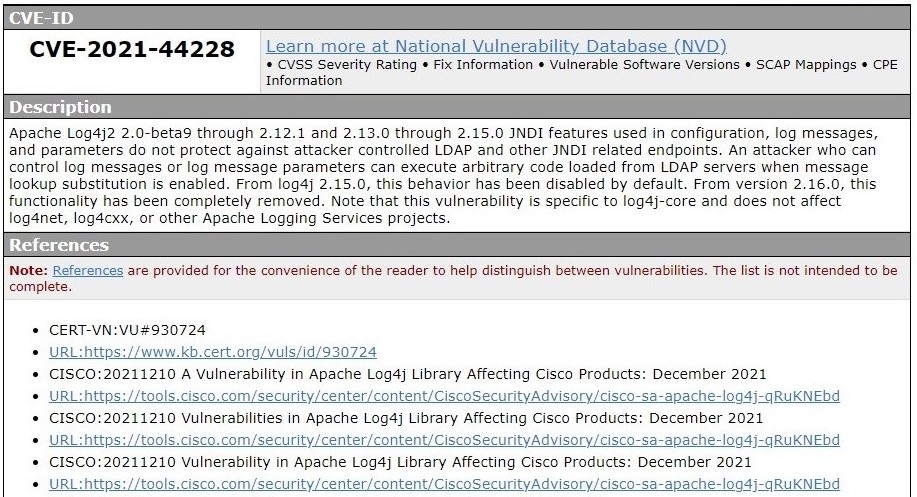
\includegraphics[width=0.98\textwidth]{fig/CVE-2021-44228-2}
    \caption{CVE平台中漏洞CVE-2021-44228}\label{fig:CVE-2021-44228}
\end{figure}

\begin{figure}[!t]
    \centering
    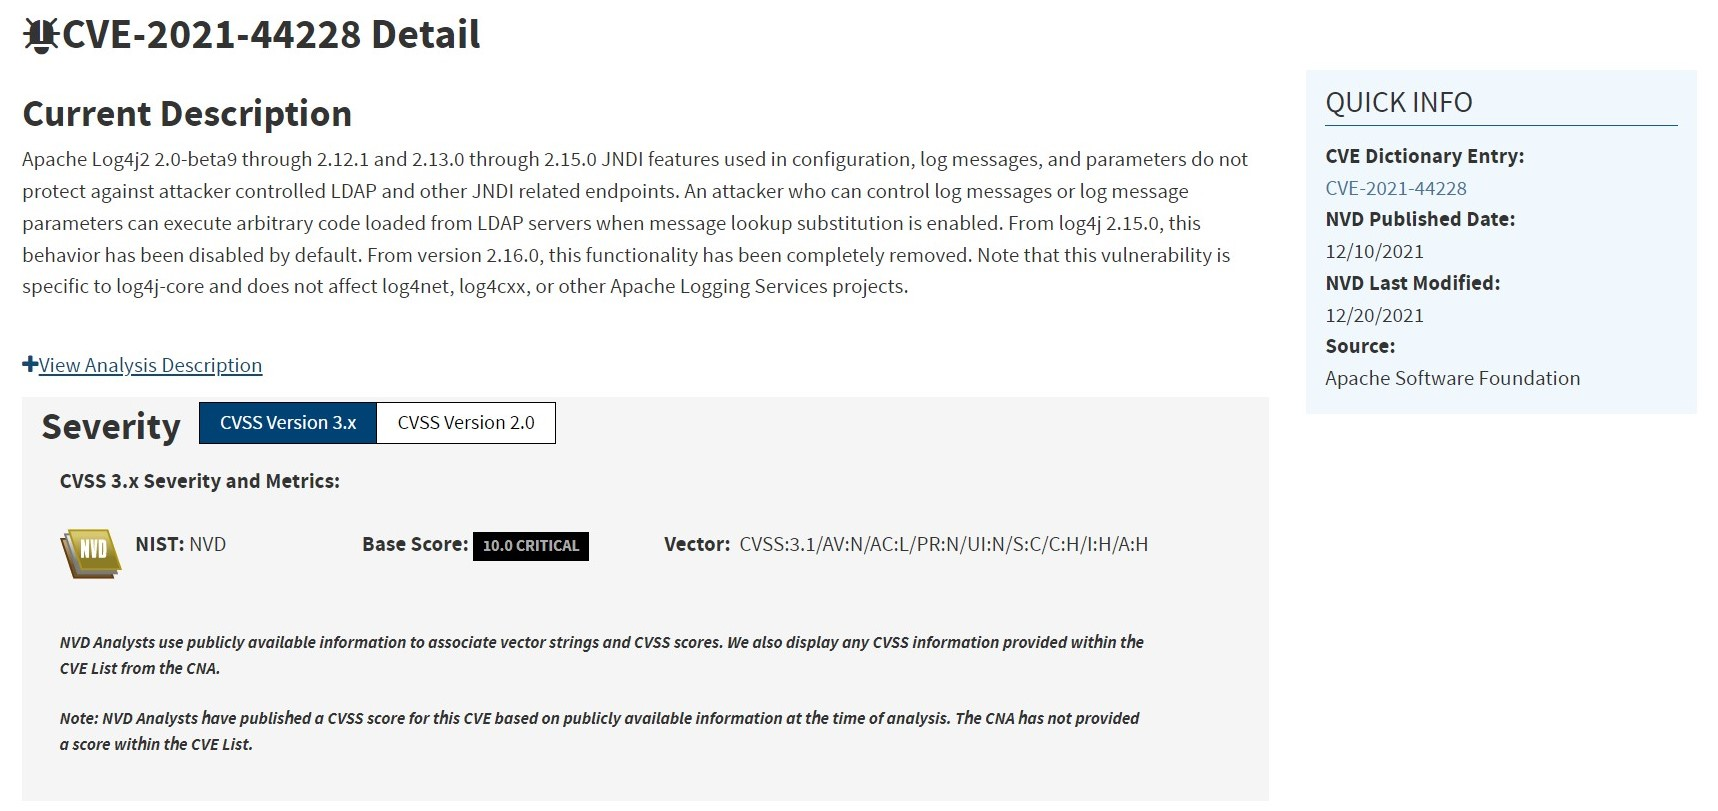
\includegraphics[width=1.0\textwidth]{fig/NVD-2021-44228}
    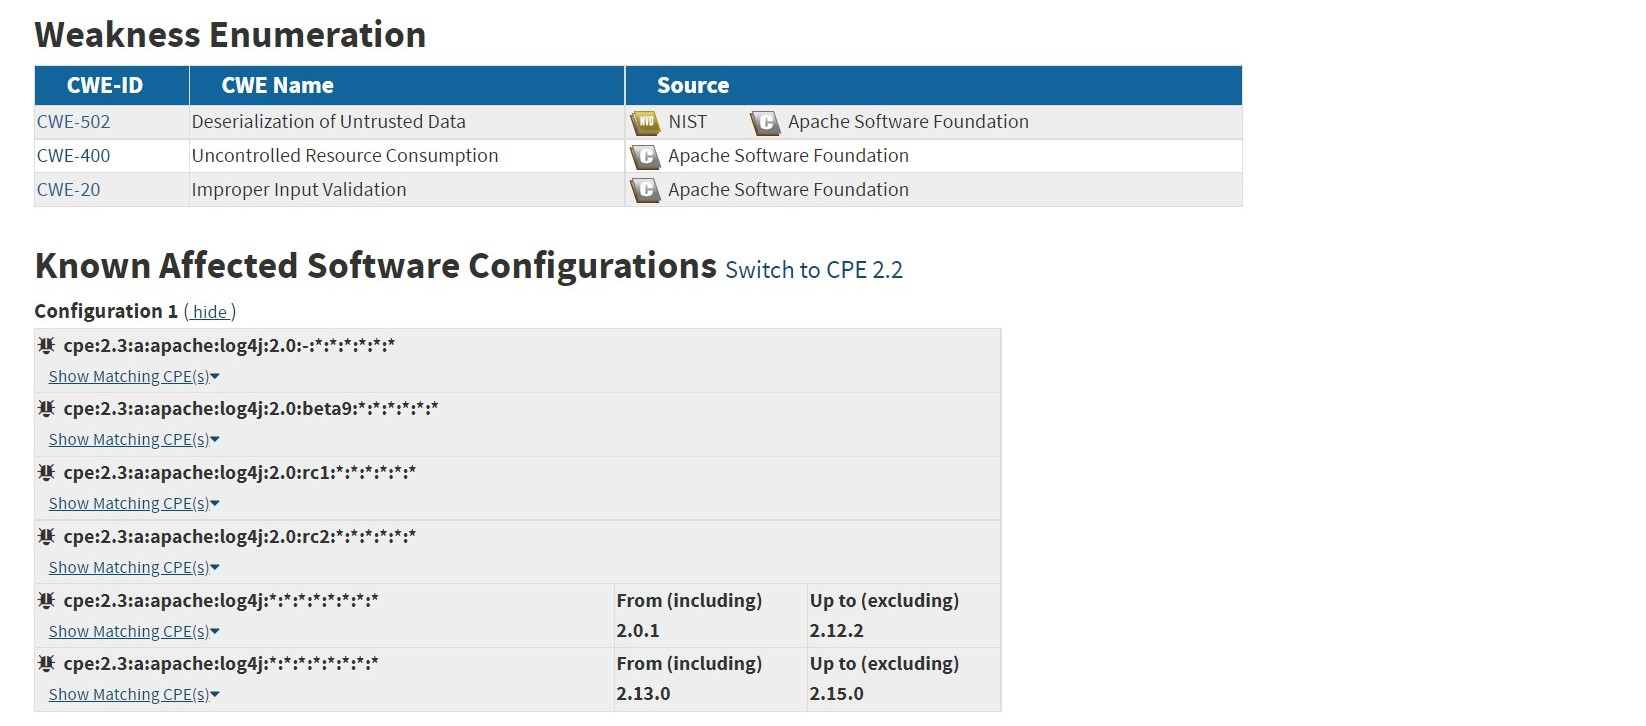
\includegraphics[width=1.0\textwidth]{fig/NVD-2021-44228-2}\caption{NVD平台中漏洞CVE-2021-44228}
    \label{fig:NVD-2021-44228}
\end{figure}

% \tocheck{可解释下CVE List,以及在NVD之后,描述下CVEdetails。}

CVE被设计作为漏洞字典用于收录并编号漏洞,这也导致CVE中漏洞信息过于精简,仅有一段漏洞描述和参考链接信息。基于CVE平台收录的漏洞条目信息,美国国家漏洞数据库(NVD)\footnote{https://nvd.nist.gov/}、中国国家信息安全漏洞库(CNNVD)\footnote{http://www.cnnvd.org.cn/}等漏洞数据库被构建。这些数据库与CVE平台数据完全同步,并为每个漏洞条目(CVE Entry)提供更丰富的信息,如:影响的软件名及版本、修复信息、严重性评分、影响评级等。图\ref{fig:NVD-2021-44228}所示为NVD平台中漏洞CVE-2021-44228\footnote{https://nvd.nist.gov/vuln/detail/CVE-2021-44228}。




\subsection{漏洞公告} 
% 是什么? 有哪些信息? 有哪些种(official、third-party)?举个例子?
漏洞公告(Advisory),也被称为漏洞通告,一般是由受漏洞影响的软件的厂商(Vendor)对外发布的安全漏洞警报,通常包含:漏洞触发描述、漏洞影响结果、漏洞软件名、软件版本等描述信息,有时也会包含漏洞发现者、漏洞问题报告(Issue Report)、漏洞补丁等知识。

\begin{figure}[!t]
    \centering
    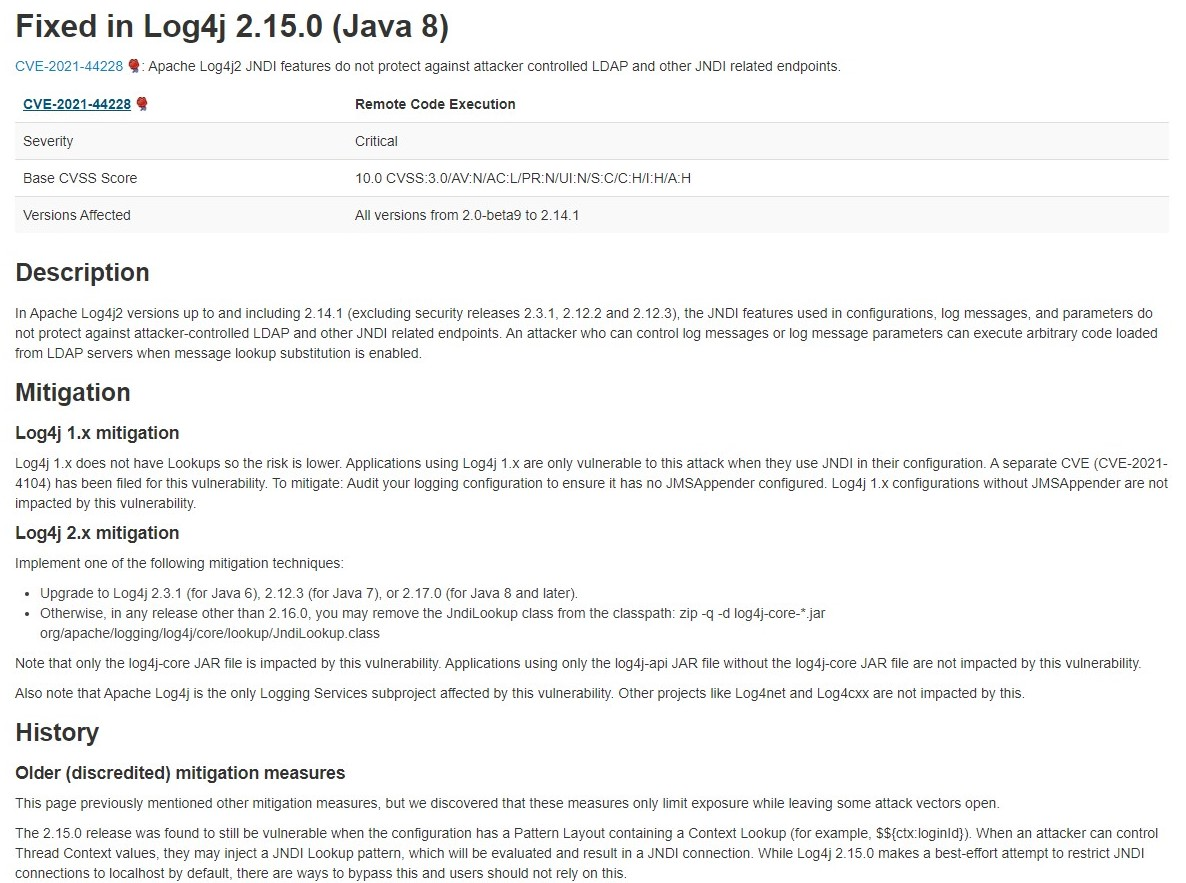
\includegraphics[width=1.0\textwidth]{fig/Vendor-2021-44228}
    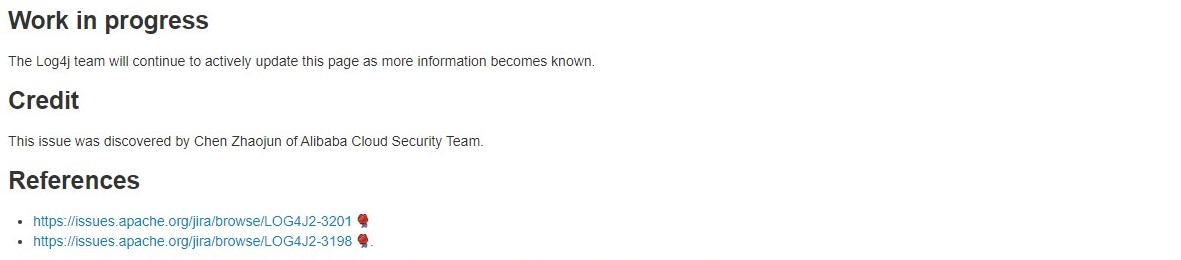
\includegraphics[width=1.0\textwidth]{fig/Vendor-2021-44228-2}
    \caption{Apache Log4j发布的漏洞CVE-2021-44228公告}
    \label{fig:Vendor-2021-44228}
\end{figure}

图\ref{fig:Vendor-2021-44228}为厂商Apache发布的关于安全漏洞CVE-2021-44228的公告\footnote{https://logging.apache.org/log4j/2.x/security.html},包含修复方式---“Log4j 2.x mitigation ...... Upgrade to Log4j 2.3.1 (for Java 6), 2.12.3 (for Java 7), or 2.17.0 (for Java 8 and later)”、漏洞发现者---“Credit:This issue was discovered by Chen Zhaojun of Alibaba Cloud Security Team.”、参考链接---“https://issues.apache.org/jira/browse/LOG4J2-3198”等信息。


以上介绍的由厂商发布的漏洞公告,也被称为:厂商公告(Vendor Advisory)。由于某一厂商只会发布、维护与该厂商相关的软件漏洞通告,而开源社区的开发人员难以一一关注所有厂商的公告信息,因此,出现了许多致力于收集并维护所有漏洞公告信息的第三方平台。这些由第三方平台收集并维护的漏洞公告也被称为:第三方公告(Third-Party Advisory)。目前,认可度较高、影响力较大的第三方漏洞公告平台有Red Hat\footnote{https://access.redhat.com/errata/}、Debian\footnote{https://www.debian.org/security/}、Gentoo\footnote{https://security.gentoo.org/}等。

% 官方或第三方?再顺路引出相关的sources,作为例子。

% Vender advisory, official advisory:CVE NVD,third-party advisory:Redhat debian 啥啥
% 是什么? 有哪些信息? 有哪些种(official、third-party:权威或非权威啥啥啥。。。社区、工业啥啥、、、)?举个例子?

\begin{figure}[!t]
    \centering
    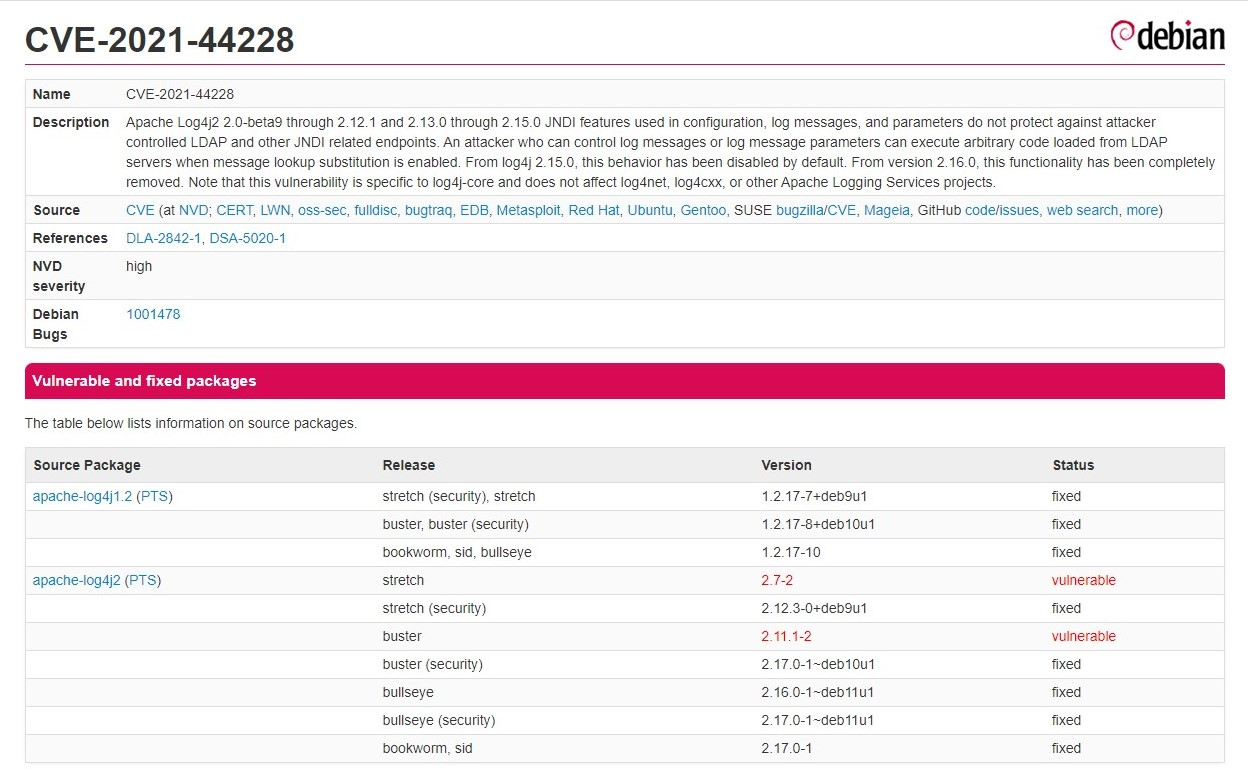
\includegraphics[width=1.0\textwidth]{fig/debian-2021-44228}
    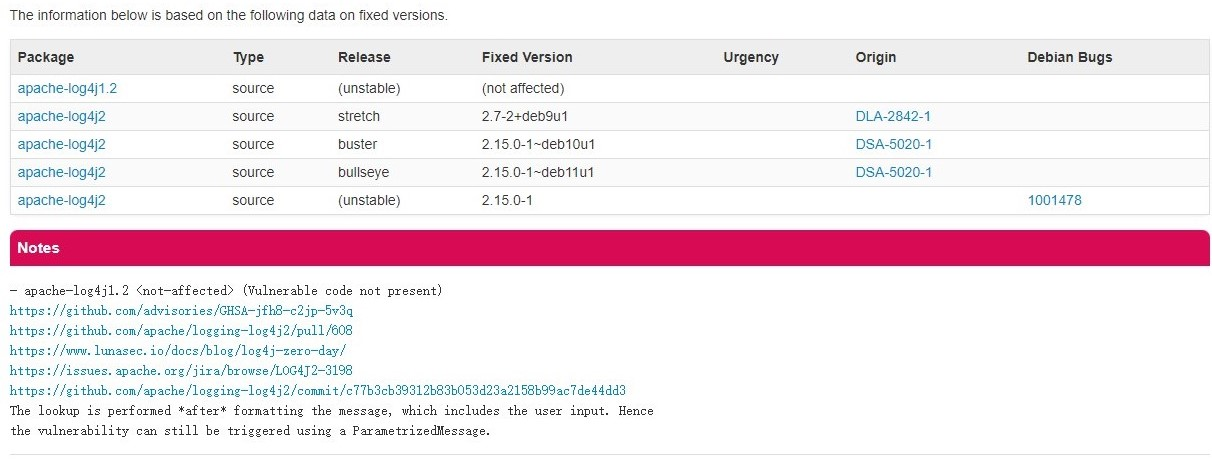
\includegraphics[width=1.0\textwidth]{fig/debian-2021-44228-2}
    \caption{Debian平台中漏洞CVE-2021-44228的公告}
    \label{fig:debian-2021-44228}
\end{figure}
图\ref{fig:debian-2021-44228}为Debian平台中漏洞CVE-2021-44228的公告\footnote{https://security-tracker.debian.org/tracker/CVE-2021-44228},其中还包括了该漏洞的补丁c77b3c@logging-log4j2\footnote{https://github.com/apache/logging-log4j2/commit/c77b3cb39312b83b053d23a2158b99ac7de44dd3}(即图中“Note”引用的参考链接),这在NVD和Vendor Advisory中都未出现。


\subsection{漏洞补丁}
补丁(Patch),也称:补丁程序,是指对计算机程序进行的一组更改,旨在更新其功能或修复其缺陷。漏洞补丁(Vulnerability Patch)则指为修复程序中的安全漏洞所开发的补丁,通常是Git和SVN中的代码提交(Commit),或是文本文件(.patch文件)形式。对于代码提交形式的补丁,后文中将简称为补丁提交。

\begin{figure}[!t]
    \centering
    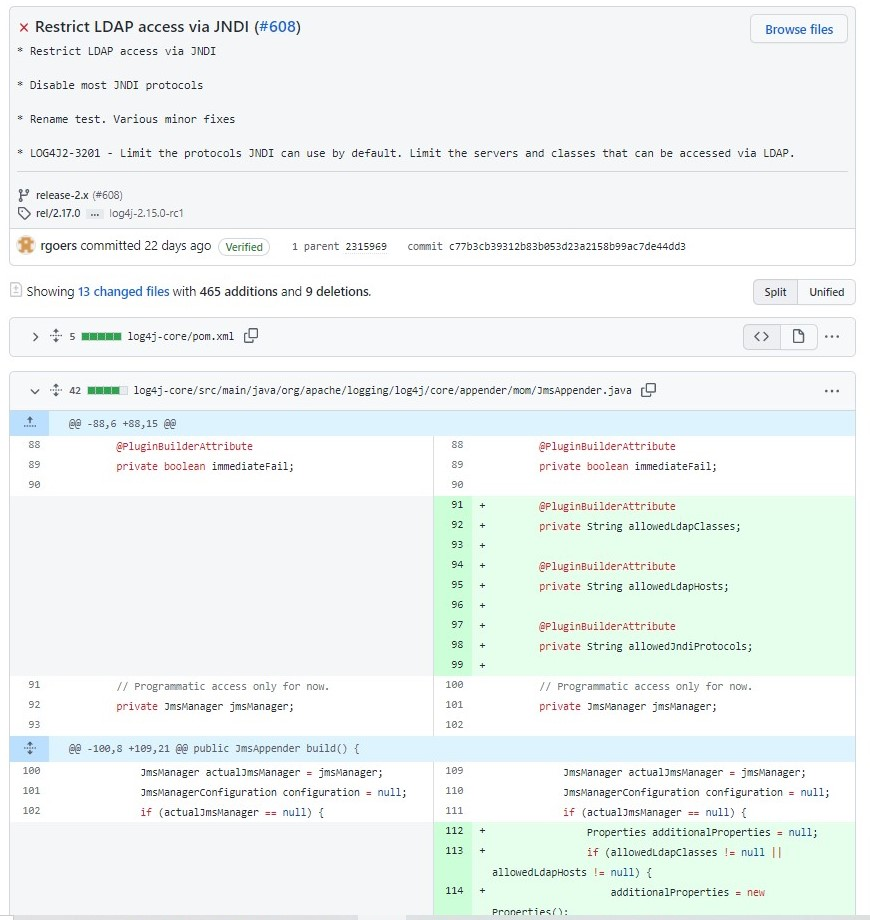
\includegraphics[width=0.95\textwidth]{fig/commit-2021-44228}
    \caption{漏洞CVE-2021-44228的Github Commit补丁}
    \label{fig:commit-2021-44228}
\end{figure}

例如,上图\ref{fig:debian-2021-44228}中的参考链接“https://github.com/apache/logging-log4j2/commit/\\c77b3cb39312b83b053d23a2158b99ac7de44dd3”,即为漏洞CVE-2021-44228的补丁提交,该提交的内容见图\ref{fig:commit-2021-44228}。


\section{相关工作}
本文将从漏洞信息质量、漏洞补丁识别和漏洞补丁应用三个方面介绍相关的研究工作。

\subsection{漏洞信息质量}
随着社区、工业界及学术界构建的漏洞数据库越来越多,数据库中积累的漏洞数据也越来越多,研究人员开始关注数据库中漏洞信息的质量。

Nguyen和Massacci\cite{nguyen2013reliability}最早揭示了NVD数据库中软件版本信息的不准确情况。为了提高这项信息的可靠性,Nguyen\cite{nguyen2016automatic}和Dashevskyi等人\cite{dashevskyi2018screening}提出方法,用以确定某一软件的旧版本是否会受到新披露漏洞的影响。他们认为:如果软件的旧版本包含修复漏洞所更改的代码行,则该版本被视为受新披露的漏洞影响。
不同于以上工作的方法,Dong等人\cite{dong2019towards}从漏洞的描述信息中识别受漏洞影响的软件名称和版本,并与漏洞报告所提供的软件名称和版本信息进行对比,以此发现不一致、不准确的软件版本信息。他们发现,NVD等多个漏洞数据库中会遗漏真正受漏洞影响的版本,也会错误地包含了不受漏洞影响的版本。

除了受漏洞影的软件版本信息,Mu等人\cite{mu2018understanding}揭示了漏洞报告中,普遍缺失用于重现漏洞的关键步骤。Chaparro等人\cite{chaparro2017detecting}提出方法用于检测漏洞描述中是否缺少用于重现漏洞的关键步骤及预期结果信息。以上工作主要侧重于漏洞的软件版本及漏洞重现的信息,而本文则重点关注漏洞数据库中的补丁知识,并尝试自动化地从多个知识源的漏洞公告信息中定位漏洞补丁。
% \tocheck{jo等人}\cite{jo2020gapfinder}识别网络安全领域内的语义不一致。
% \tocheck{这些工作侧重于漏洞信息的不同方面。按照这个方向,我们的工作重点是漏洞补丁,并尝试从漏洞报告的综合来源中识别漏洞补丁。}

Tan等人完成了一项与本文的研究问题较为相似的工作\cite{Tan2021locating}。他们使用深度学习排名算法对代码仓库中的代码提交进行排名,把排在首位的代码提交作为漏洞的补丁提交。他们的工作包含两个假设:(1)受漏洞影响的软件的代码仓库已知,(2)漏洞与其补丁提交在数量上是一对一的映射关系。然而,事实上,受漏洞影响的软件的代码仓库并不全部已知,而需人工识别。此外,漏洞与其补丁提交在数量上存在一对多的关系(见章节\ref{sec:cardinality})。所以,该方法对于开源软件漏洞不具有通用性。


% \subsection{漏洞补丁分析}
% 当前,有多中补丁分析相关的任务可用于提高软件安全性,如:补丁的生成和部署\cite{mulliner2013patchdroid,duan2019automating,xu2020automatic}、补丁的存在性测试\cite{zhang2018precise,jiang2020pdiff,dai2020bscout}以及秘密补丁识别\cite{xu2017spain,zhou2017automated,sabetta2018practical,chen2020machine}。

% 此外,研究人员也已为Java\cite{ponta2019manually}、C/C++\cite{fan2020ac}以及特定开源项目\cite{jimenez2018enabling}构建安全补丁数据集。基于这些数据集,研究人员已开展实证研究以表征漏洞及其补丁\cite{zaman2011security,li2017large,liu2020large,antal2020exploring}。在这些工作中,补丁多由人工识别\cite{xu2020automatic,jiang2020pdiff,dai2020bscout,xu2017spain,zhou2017automated,sabetta2018practical,chen2020machine,ponta2019manually,zaman2011security},或通过启发式规则识别,例如:在CVE的参考链接中查找补丁提交信息\cite{duan2019automating,fan2020ac,jimenez2018enabling,li2017large,liu2020large},以及在提交信息(Commit Message)中搜索CVE标识符\cite{fan2020ac, jimenez2018enabling, antal2020exploring}。这些工作存在的问题为:通过人工收集成本过高,且耗时较长;然而,启发式规则的方法又不足以找到或是找全补丁。

\subsection{漏洞补丁识别}
随着披露的开源软件漏洞越来越多、漏洞影响越来越大,为了能够及时获取补丁知识,许多自动化的补丁识别方法被提出。

周鹏等人\cite{9周鹏2022一种}提出了一种针对Linux内核的安全漏洞修复补丁自动识别方法,该方法通过持续收集并标注安全漏洞补丁数据,以及定义并抽取原始补丁文件的特征,来训练一个可识别安全漏洞修复补丁的分类器。邹雅毅等人\cite{7邹雅毅2016开源软件漏洞补丁的采集与整理}针对Linux内核、Ffmpeg、Wireshark三个项目设计了一种DIFF文件形式的补丁采集方法。该方法通过定义的DIFF特征来识别补丁链接,并基于与补丁链接出现在同一页面的CVE ID来完成漏洞及其修复补丁映射关系的确认。

李瑞科等人\cite{10李瑞科20191999}构建了一个包括近20年漏洞数据的安全漏洞数据集,通过程序自动化和人工采集结合的方法采集了多个国内外知名漏洞平台1999–2018年间的安全漏洞数据,并对采集的漏洞数据进行切片和格式化操作。Li和Vern\cite{li2017large}基于NVD平台的漏洞数据,通过收集带有Git代码提交链接的漏洞,实现漏洞补丁数据集的构建。同样,Liu等人\cite{liu2020large}也是基于CVE和NVD漏洞报告中参考链接的数据,解析并识别GitHub代码提交的链接作为漏洞补丁。Ponta等人\cite{ponta2019manually}通过人工手动收集的方式,构建一个针对Java语言,包含205个开源项目、624个漏洞、1282个补丁的数据集。

Fan等人\cite{fan2020ac}针对Google Chrome、 Linux和 Google Android项目构建了一个C及C++语言的漏洞数据集。通过分析CVE Details漏洞报告中带有Git仓库的参考链接,确定该漏洞所影响软件的仓库,并以CVE ID及Bug ID作为关键词在该仓库的代码提交历史中搜索修复该漏洞的补丁。类似地,Jimenez等人\cite{jimenez2018enabling}提出了一种自动补丁识别框架--VulData7,并构建了一个针对Linux Kernel、WireShark、OpenSSL和 SystemD四个项目的漏洞补丁数据集。该框架也是以CVE ID及Bug ID作为关键词在该仓库的代码提交历史中搜索修复该漏洞的补丁。

上述工作提出的补丁识别方法,多是通过基于启发式规则从漏洞公告的参考链接或项目的历史代码提交中识别补丁。这些方法多是针对特定的程序语言或项目而设计,较为局限,无法适用于所有安全漏洞。


\subsection{漏洞补丁应用}
漏洞补丁可被用于多种软件安全性任务。例如,补丁存在性检测\cite{8文琪2020}、基于漏洞补丁生成漏洞攻击程序\cite{brumley2008automatic,you2017semfuzz}、基于漏洞补丁进行漏洞影响分析\cite{4李舟军2015软件安全漏洞检测技术,5李韵2020基于机器学习的软件漏洞挖掘方法综述,pashchenko2018vulnerable,ponta2020detection,pashchenko2020vuln4real,Wang2020empirical} 以及基于漏洞补丁进行漏洞检测\cite{li2016vulpecker,li2018vuldeepecker,zhou2019devign,jimenez2019importance}。%、通过匹配漏洞签名\cite{jang2012redebug,kim2017vuddy}、通过匹配漏洞和补丁检测签名\cite{xu2020patch,xiao2020mvp,cui2020vuldetector}来检测程序中的漏洞。

文琪等人\cite{8文琪2020}提出一个名为PatchChecker的基于关键路径和语义的漏洞补丁存在性检测方法。该方法通过识别漏洞的修复路径及其程序修复前后的语义特征,生漏洞补丁的签名。基于补丁签名,在目标程序中识别对应路径并进行比较,以判断漏洞补丁是否被应用。%基于安全漏洞的补丁数据,Li等人\cite{[16]}提出了一种可扩展的漏洞检测方法,该方法使用一种可扩展的基于语法的方法来识别克隆的漏洞代码。
Li等人\cite{li2016vulpecker}提出了一种基于代码相似度分析的自动化漏洞检测方法。给定漏洞,该方法先抽取该漏洞补丁中的代码特征,再利用代码相似度算法检测项目中相似的代码,实现漏洞检测。之后,Li等人\cite{li2018vuldeepecker}又提出了一种基于深度学习系统的漏洞检测方法。Kim等人\cite{kim2017vuddy}提出了一种可扩展的克隆代码的安全漏洞检测方法。该方法利用函数级代码和基于长度过滤技术,能够高效准确地检测大型软件程序中的安全漏洞。

Xu等人\cite{xu2020patch}提出了一种名为BinXray基于补丁的漏洞匹配方法,以准确有效地识别程序中的“1-day”漏洞。该方法首先通过比较漏洞修复前后的程序,基于程序块轨迹来提取补丁的签名。检测时,基于补丁语义加快签名搜索,并通过计算程序轨迹的相似性识别目标程序是否已修补。Xiao等人\cite{xiao2020mvp}提出了一种检测重现漏洞(Recurring Vulnerability)的方法,MVP。 该方法基于使用程序切片从漏洞函数的句法及语义中提取漏洞和补丁签名;在检测阶段,如果目标函数与漏洞签名匹配成功,但与补丁签名匹配不成功,则被识别为潜在漏洞。李赞等人\cite{22李赞2018}提出了一种利用补丁来提高相似性检测准确性的漏洞发现方法。该方法基于漏洞补丁,通过程序切片技术去除漏洞函数中与漏洞无关的代码,并利用程序切片生成漏洞特征来检测漏洞。李元成等人\cite{23李元诚2020}提出一种基于深度聚类算法的软件源代码漏洞检测方法。该方法先通过构造软件代码属性图,遍历代码中API序列,并将其向量化;再以关键代码为中心进行聚类,根据聚类结果判断异常函数并匹配漏洞库,从而实现漏洞代码的检测。

本文提出的方法可以为以上补丁存在性检测、漏洞影响分析、漏洞挖掘等工作提供漏洞补丁知识。


%与上一小结的补丁分析工作类似,这些工作中的CVE补丁主要通过人工识别\cite{pashchenko2018vulnerable,ponta2020detection,pashchenko2020vuln4real,xiao2020mvp}、基于启发式规则的方法\cite{li2016vulpecker,li2018vuldeepecker,you2017semfuzz,Wang2020empirical,jimenez2019importance}或直接取自为特定项目建立CVE和补丁之间映射关系的安全公告\cite{jang2012redebug,kim2017vuddy,xu2020patch}。但是,人工识别的成本过高,而且基于启发式规则的方法找到或是找全补丁。       % 背景知识与相关工作
\chapter{开源软件漏洞经验研究}\label{sec:study}

本章将主要介绍为了解当前漏洞数据库现状,考察其中漏洞补丁的质量和特征所开展的经验研究工作,包括经验研究的设计、数据准备以及经验研究的结果分析。


\section{研究设计}
\subsection{研究问题}
为了了解已有漏洞数据库中开源软件漏洞补丁的质量和特征,本文所开展的针对当前商业漏洞数据库的经验研究包含以下研究问题:

\begin{itemize}[leftmargin=*]
    \item \textbf{RQ1 补丁覆盖率分析:}当前商业漏洞数据库中,漏洞补丁信息的覆盖度如何?即,有多少漏洞包含补丁信息?(见章节\ref{sec:coverage})
    \item \textbf{RQ2 补丁一致性分析:}不用漏洞库间,漏洞补丁信息的一致性如何?即,有多少漏洞在漏洞数据库中具有相同的补丁信息?(见章节\ref{sec:consistency})
    \item \textbf{RQ3 补丁类型分析:}开源漏洞补丁的类型有哪些? (见章节\ref{sec:type})
    \item \textbf{RQ4 补丁映射分析:}开源漏洞与其补丁在数量上的映射关系是怎样的? (见章节\ref{sec:cardinality})
    \item \textbf{RQ5 补丁准确性分析:}当前商业漏洞数据库中,漏洞的补丁信息准确度如何? (见章节\ref{sec:accuracy})
\end{itemize}
    
其中,RQ1可用来评估漏洞数据库中开源软件漏洞的补丁缺失程度,RQ2用来评估不同漏洞数据库中漏洞补丁的不一致程度,RQ3和RQ4用来表征常见的补丁类型以及开源漏洞及其补丁之间的映射关系,RQ5可用来评估不同漏洞数据库中漏洞补丁信息的准确性。总的来说,RQ1、RQ2和RQ5的结果旨在从不同的角度评估补丁质量,并挖掘出对自动化补丁\tocheck{识别}方法的需求;RQ3和RQ4旨在从不同角度捕捉开源软件漏洞补丁的特征,并为自动化补丁\tocheck{识别}方法的设计提供\tocheck{启发}。

\subsection{评估标准}\label{sec:metric}
本章经验研究使用了信息检索中常用的评估标准---Precision(精确率)、Recall(召回率)和F1-Score(F1值)。

对于一个搜索或分类问题来说,样本分为“Positive(正)”和“Negative(负)”两个类别。那么,模型搜索或分类的结果就会有四种情况:
\begin{itemize}
    \item True Positive(真阳性),表示:将正样本预测为正样本,即数据库提供的或工具返回的正确补丁信息。
    \item True Negative(真阴性),表示:将负样本预测为负样本,即数据库未提供的或工具未返回的错误补丁信息。
    \item False Positive(假阳性),表示:将负样本预测为正样本,即数据库提供的或工具返回的错误补丁信息。
    \item False Negative(假阴性),表示:将正样本预测为负样本,即数据库未提供的或工具未返回的正确补丁信息。
\end{itemize}

\textbf{Precision(精确率),}用于衡量数据库提供的补丁中正确补丁的比率,或是工具返回结果中正确补丁的比率,计算公式如下:
\begin{equation}\label{eq:precision}
    Precision=\frac{True\ Positive}{True\ Positive + False\ Positive} 
\end{equation}

\textbf{Recall(召回率),}用于衡量正确补丁在数据库中被提供的比率,或是正确补丁被工具返回的比率,计算公式如下:
\begin{equation}\label{eq:recall}
    Recall=\frac{True\ Positive}{True\ Positive + False\ Negative} 
\end{equation}

\textbf{F1-Score(F1值),}用以中和表示Precision及Recall的结果;因为Precision仅仅反映精确率,Recall仅仅反映召回率,无法反映总体评估结果,F1-Score计算公式如下:
\begin{equation}\label{eq:f1}
    F1-Score=2*\frac{Precision*Recall}{Precision + Recall} 
\end{equation}

\section{数据准备}\label{sec:preparation}
\subsection{漏洞数据库选择}
为挑选高质量的、具有代表性的漏洞数据库作为研究对象,本文前期调研了来自安全领域的社区、工业界和学术界的漏洞数据库。在该章节的经验研究工作中,本文首先排除了来自安全社区的数据库(例如,CVE List和NVD)。因为这两个数据库不提供结构化的补丁信息,而补丁链接多是隐藏在参考链接中;此外,CVE List和NVD数据库中不仅仅包含开源软件漏洞,还包括闭源软件、系统及硬件相关的漏洞。本文还排除了来自学术界的数据集\cite{ponta2019manually,fan2020ac,jimenez2018enabling,gkortzis2018vulinoss,namrud2019androvul,li2017large,liu2020large,antal2020exploring},这是因为这些数据集中的漏洞通常限定于特定的一两种程序语言(例如:Python、Java),而非面向所有开源软件,缺乏多样性不具有代表性;此外,由于长期缺乏维护,这些漏洞数据集缺失较新的漏洞数据。


对于工业界的数据库,本文首先关注到BlackDuck\cite{blackduck}、WhiteSource\cite{whitesource}、Veracode\cite{veracode}和Snyk\cite{snyk}四家安全公司提供软件成分分析(Software Composition Analysis)服务,这种服务通过识别并分析当前软件系统中使用的开源成本(即第三方库),报告所使用的开源成分中的漏洞。因此,这四家公司需要先构建尽可能完整且包含详细漏洞信息的漏洞库作为服务基础,本文便首先将这四家公司的漏洞数据库作为研究对象。截至2021年4月5日,收集的信息为:

\begin{itemize}[leftmargin=*]
\item\textbf{Black Duck,}该公司的报告显示:该公司的安全公告中共包含157,000多个漏洞,涵盖90多种编程语言,其中,数千个漏洞尚未被NVD收录。该公司的漏洞数据库由特定的专家团队进行维护,以确保漏洞数据的完整性和准确性,然而,该公司的漏洞数据信息并未对外公开。
\item\textbf{Sonatype\footnote{https://ossindex.sonatype.org},} 该公司声称:\textit{“OSS Index是一个免费的开源组件目录,其中的扫描工具可帮助开发人员识别漏洞、了解风险并确保其软件安全。”}\footnote{英文原文为:"OSS Index is a free catalogue of open source components and scanning tools to help developers identify vulnerabilities, understand risk, and keep their software safe."} Sonatype的OSS Index支持20多个生态系统(如:Maven、npm、Go、PyPI等)。该公司公开的漏洞信息包括漏洞描述、受漏洞影响的组件和版本、CVSS向量、参考链接等信息。
\item\textbf{WhiteSource\footnote{https://www.whitesourcesoftware.com/vulnerability-database/},}该公司从NVD及其他安全公告平台和问题追踪系统(issue tracking system)中共收集的漏洞超过175,000个,涵盖200多种编程语言。
\item\textbf{Veracode\footnote{https://sca.analysiscenter.veracode.com/vulnerability-database},}该公司的漏洞数据库涵盖10多种编程语言相关的18,000多个漏洞,公开的漏洞信息包括受漏洞影响的组件和版本范围、库修复说明、参考资料等。
\item\textbf{Snyk\footnote{https://snyk.io/vuln},}该公司声称:漏洞数据库\footnote{https://snyk.io/product/vulnerability-database/}是由经验丰富的安全研究团队持续维护,通过关注安全公告、Jira issue报告,GitHub Commits等方式自动识别安全漏洞相关的报告。该公司的数据库涵盖超过10个编程语言生态系统,如:Maven、npm、Go、Composer等。该数据库提供漏洞的详细信息,包括受漏洞影响的组件、版本范围、修复方法、参考链接等。
% \item \textbf{Gitlab Security} GitLab 咨询数据库是 Gitlab 依赖扫描器\footnote{https://docs.gitlab.com/ee/user/application\_security/dependency\_scanning/index.html} 的基础。目前涵盖了 6000 多个 CVE 条目和 8 个生态系统(即 Nuget、Conan、Maven 等)。提供了详细信息,例如描述、受影响的组件和版本、解决方案和参考。
\end{itemize}

进一步调研后发现,这四家公司中某些公司并未公开漏洞数据库,或是公开的漏洞信息中不包含用于修复漏洞的补丁信息,这将无法达成研究目标。最终,本文选择了两家公司的漏洞数据库作为研究对象,下文中简称为:$DB_A$和$DB_B$。


\subsection{广度数据集构建}
为了评估漏洞数据库中补丁的缺失程度以及不同数据库间补丁的不一致性(即RQ1和RQ2),本文基于$DB_A$和$DB_B$构建了一个开源软件漏洞的广度数据集用以实验分析。截至2020年4月7日,分别从$DB_A$和$DB_B$中分别获取了\tocheck{8,630}和\tocheck{5,858}个CVE漏洞。

\subsection{深度数据集构建}
为了表征漏洞补丁的类型、映射关系以及尽可能准确地评估补丁信息的准确性(即RQ3、RQ4和RQ5),本文还基于$DB_A$和$DB_B$的数据,构建了一个开源软件漏洞的深度数据集。该数据集的漏洞数量少于广度数据集,但每个漏洞都包含由人工确认的补丁信息。%为了确保漏洞补丁信息完整性和准确性,其中所有漏洞的补丁信息都是由人工识别。

在该深度数据集的构建过程中,为了确保数据集能够涵盖足够多的漏洞用以实验评估,但又不至于在人工识别补丁的阶段产生难以完成的工作量,本文仅将在$DB_A$和$DB_B$都含有补丁信息的漏洞列入该深度数据集,最终,该深度数据集共包含\tocheck{1,417}个CVE漏洞。



然后,对于该深度数据集中的每个CVE漏洞,首先分别由两位研究人员通过分析$DB_A$和$DB_B$数据库报告的补丁、查看NVD中的漏洞描述和参考链接信息以及搜索GitHub代码仓库的提交历史和其他网络资源等方式,独立得找到其补丁信息;之后,对比由两位研究人员独立查找得到得补丁信息,对于补丁结果不一致的漏洞,两位研究人员再一起分析讨论直到达成共识。这两位研究人员分别是本文作者和与本文作者同课题组的学生。由于公开的信息有限,\tocheck{1,417}个CVE漏洞中的\tocheck{122}个CVE漏洞无法找到补丁信息,比如:漏洞CVE-2016-3942在NVD中没有漏洞报告,但$DB_A$和$DB_B$将 jsrender@f984e1\cite{jsrender}标识为其补丁,两位研究人员无法确认该补丁信息的准确性。最终,该深度数据集共包含了\tocheck{1,295}个CVE漏洞。

\begin{figure*}[h]
    \centering
    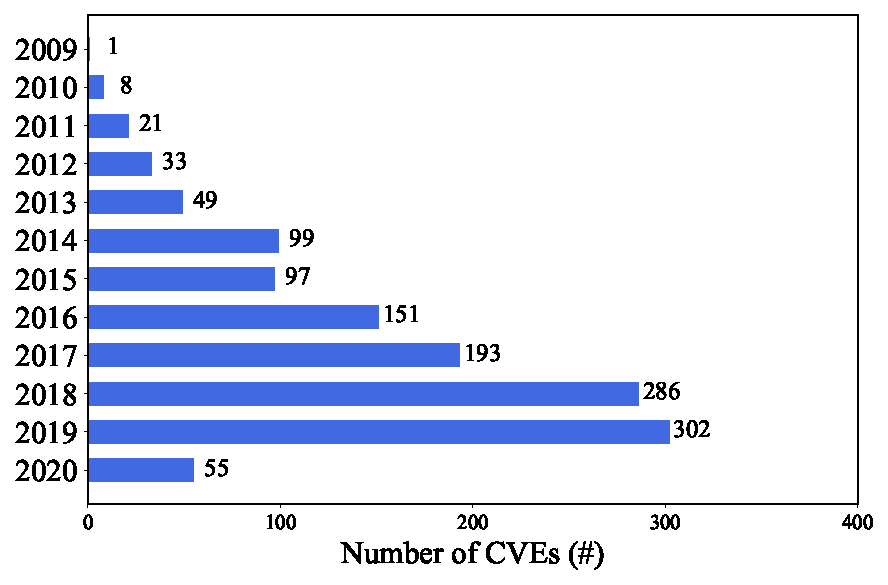
\includegraphics[scale=0.85]{fig/rq0-year.pdf}
    %\vspace{-5pt}
    \caption{数据集中漏洞年份统计}\label{fig:rq0-year}
\end{figure*}

\begin{figure*}[t]
    \centering
    \includegraphics[scale=0.85]{fig/rq0-language.pdf}
    \caption{数据集中漏洞程序语言分布统计}\label{fig:rq0-language}
\end{figure*}

\begin{figure}[t]
    \centering
    \begin{subfigure}[b]{0.45\textwidth}
    \centering
    \includegraphics[scale=0.98]{fig/rq1-CVE-IDs-VS.pdf}
    %\vspace{-5pt}
    \caption{开源软件漏洞}\label{fig:rq1-cves}
    \end{subfigure}
    \begin{subfigure}[b]{0.45\textwidth}
    \centering
    \includegraphics[scale=0.98]{fig/rq1-CVE-IDs-Patches-VS.pdf}
    %\vspace{-5pt}
    \caption{含补丁信息的开源软件漏洞}\label{fig:rq1-cves-with-patches}
    \end{subfigure}
    %\vspace{-10pt}
    \caption{$DB_A$与$DB_B$间数据交集}\label{fig:intersection}
\end{figure}


本文还进一步分析了该深度数据集中\tocheck{1,295}个CVE开源软件漏洞的年份和程序语言分布情况,以评估该数据集是否具有代表性。如图\ref{fig:rq0-year}所示,CVE的数量逐年增加,这与Snyk的报告\cite{Snyk-report}一致。此外,本文通过分析补丁中更改的源文件类型来确定CVE的编程语言。如图\ref{fig:rq0-language}所示,深度数据集中的CVE漏洞涵盖了七种较为常用的程序语言,具有较好的语言多样性。因此,可以认为该深度数据集对于开源软件漏洞数据库具有较好的代表性。


\section{RQ1:覆盖率分析}\label{sec:coverage}

如图\ref{fig:rq1-cves}所示,$DB_A$和$DB_B$数据库中共有的CVE漏洞为\tocheck{4,418}个,同时$DB_A$和$DB_B$分别包含\tocheck{4,212}和\tocheck{1,440}个特有的CVE漏洞;如图\ref{fig:rq1-cves-with-patches}所示,$DB_A$中\tocheck{3,607(41.8\%)}的CVE漏洞含有补丁信息,$DB_B$中\tocheck{2,412(41.2\%)}的CVE漏洞含有补丁信息;$DB_A$和$DB_B$数据库共有\tocheck{10,070}个开源软件CVE漏洞,而其中仅有\tocheck{4,602(45.7\%)}的漏洞提供了补丁信息。

% \begin{figure}[h]
%     \centering
%     \includegraphics[scale=0.98]{fig/rq1-CVE-IDs-VS.pdf}
%     \caption{开源软件漏洞数据}\label{fig:rq1-cves}
% \end{figure}

% \begin{figure}[h]
%     \centering
%     \includegraphics[scale=0.98]{fig/rq1-CVE-IDs-Patches-VS.pdf}
%     \caption{补丁信息的开源软件漏洞数据}\label{fig:rq1-cves-with-patches}
% \end{figure}

由此可见,数据库$DB_A$和$DB_B$中开源软件漏洞的补丁覆盖率都较低,分别为41.8\%和41.2\%,漏洞补丁缺失的情况较为普遍。%而且可以看出,不同的漏洞数据库对\congyingEdit{OSS}漏洞的覆盖范围不同。
同时,这也体现出自动化补丁查找方法的必要性,可用于填补数据库中缺失的补丁信息。


\section{RQ2:一致性分析}\label{sec:consistency}

\begin{table}[h]
    \centering
    \small
    \caption{补丁一致性结果}\label{table:consistency}
    %\vspace{-10pt}
    \begin{tabular}{|*{1}{C{4.4em}}|*{1}{C{3.6em}}*{1}{C{5.0em}}*{1}{C{5.0em}}|*{1}{C{3.6em}}*{1}{C{4.8em}}*{1}{C{5.0em}}|}
    \noalign{\hrule height 1pt}
    \multirow{2}{*}{补丁一致} & \multicolumn{3}{c|}{存在性不一致} & \multicolumn{3}{c|}{内容不一致} \\\cline{2-4}\cline{5-7}
     & 总数 & 无漏洞信息 & 无补丁信息 & 总数 & 包含关系 & 非包含关系 \\\noalign{\hrule height 1pt}
    % \multirow{2}{*}{Cons.} & \multicolumn{3}{c|}{Existence Inconsistency} & \multicolumn{3}{c|}{Content Inconsistency} \\\cline{2-4}\cline{5-7}
    % & Total & No CVE & No Patch & Total & Inclusion & Difference \\\noalign{\hrule height 1pt}
    907 (19.7\%) & 3,185 (69.2\%) & 1,392 (30.2\%) & 1,793 (39.0\%) & 510 (11.1\%) & 176 (3.8\%) & 334 (7.3\%)\\
    % $DB_{A}$ vs. $DB_{C}$ & 3,659 & 73 (2.0\%) & 3,540 (96.7\%) & 2,523 (69.0\%) & 1,017 (27.8\%) & 46 (1.3\%) & 15 (0.4\%) & 31 (0.8\%) \\
    % $DB_{B}$ vs. $DB_{C}$ & 2,490 & 75 (3.0\%) & 2,397 (96.3\%) & 1,687 (67.8\%) & 710 (28.5\%) & 18 (0.7\%) & 7 (0.3\%) & 11 (0.4\%)\\
    \noalign{\hrule height 1pt}
    \end{tabular}
\end{table}

为了分析两个数据库之间的补丁信息一致性情况,本节主要关注带有补丁的CVE漏洞,即图\ref{fig:rq1-cves-with-patches}中的CVE漏洞。考虑到漏洞补丁的个数可能不唯一(即可能为一组补丁集),所以仅当两个数据库针对同一漏洞提供的补丁集完全相同时,才判定为补丁信息一致。本节将补丁信息不一致分为存在性不一致和内容不一致两种情况。前者是指某一个数据库为该CVE漏洞提供了补丁信息,而另一个数据库却不存在该CVE信息,或是存在该CVE却不存在相关补丁信息;后者是指两个数据库都存在该CVE的补丁信息,但它们的补丁集并不完全一致,分为包含关系或非包含关系的不一致。这两种情况分别反映了出数据库$DB_A$和$DB_B$中开源软件漏洞及其补丁信息的不完整性,以及漏洞补丁信息可能是不准确的


表\ref{table:consistency}中展示了补丁一致性分析的结果。其中,第一列为在$DB_A$和$DB_B$中具有一致补丁集的CVE数量(907,19.7\%),第二至四列为补丁存在性不一致的CVE数量(3,185,69.2\%),最后三列为都存在补丁信息但补丁集内容不一致的CVE数量(510,11.1\%)。可以发现:\tocheck{4,602}个CVE中,(1)只有\tocheck{907(19.7\%)}的漏洞在$DB_A$和$DB_B$中有一致的补丁信息;(2)超过三分之二(即\tocheck{3,185(69.2\%)})的CVE漏洞在数据库$DB_A$和$DB_B$中存在补丁信息不一致的情况,其中\tocheck{1,392(30.2\%)}的CVE漏洞不在$DB_{A}$或$DB_{B}$中,\tocheck{1,793(39.0\%)}的CVE漏洞都存在于$DB_{A}$和$DB_{B}$中但在某一数据库中无补丁信息;(3)\tocheck{510(11.1\%)}的CVE漏洞补丁信息都存在于$DB_{A}$和$DB_{B}$中补丁集内容不一致,其中,\tocheck{176(3.8\%)}CVE的来自于某一个数据库的补丁集包含来自另一个数据库的补丁集,\tocheck{334(7.3\%)}CVE的来自$DB_{A}$和$DB_{B}$的补丁集即不同也不包含。

这些结果表明,$DB_A$和$DB_B$间存在较多的补丁信息不一致情况,进而表明数据库中补丁信息的准确性也需要进一步评估。


\section{RQ3:补丁类型分析}\label{sec:type}

在\tocheck{\ref{sec:preparation}小节}中,基于人工收集的深度数据集共包含\tocheck{1,295}个CVE漏洞及\tocheck{3,043}个补丁,本小节将基于该数据集分析漏洞的补丁类型。分析结果表明,\tocheck{3,043}个补丁中,\tocheck{2,852(93.7\%)}的补丁都是为GitHub Commit形式,这可能是因为GitHub在开源软件中被广泛使用;另外\tocheck{136(4.5\%)}的补丁为SVN Commit形式,仅有\tocheck{55(1.8\%)}的补丁为来自其他Git平台的commit形式。

此外,从CVE的角度来看,\tocheck{1,295}个CVE中\tocheck{1,202(92.8\%)}的CVE有GitHub Commit类型的补丁,\tocheck{4(0.3\%)}的CVE有SVN Commit类型的补丁。由于很多项目是从SVN切换为Git管理,\tocheck{48(3.7\%)}的CVE既有GitHub Commit又有SVN Commit类型的补丁。只有\tocheck{30(2.3\%)}的CVE的补丁都为来自其他Git平台的commit形式。以上分析结果表明,开源软件漏洞的补丁类型主要为GitHub Commit,少部分为SVN Commit,而极小部分为其他Git平台的commit。

\section{RQ4:补丁映射分析}\label{sec:cardinality}
\begin{figure}[h]
\centering
\includegraphics[scale=0.80]{fig/rq4-cardinality.pdf}
\vspace{-10pt}
\caption{CVE及其补丁间映射关系统计}\label{fig:rq4-cardinality}
\end{figure}

基于深度数据集中\tocheck{1,295}个CVE漏洞及其补丁数据,本节将分析开源漏洞及其补丁间在数量上的映射关系。本文将CVE与其补丁之间的映射关系分为三种类型:一对一、\tocheck{一对一组}及一对多。

\textbf{一对一:}是指一个CVE漏洞与其补丁在数量上为一对一的关系,即一个CVE漏洞只需一个补丁即可修复,后文中简记为:\textit{SP}(Single Patch)。如图\ref{fig:rq4-cardinality}所示,深度数据集中\tocheck{567(43.8\%)}的CVE与其补丁具有一对一的映射关系(\textit{SP})

\textbf{\tocheck{一对一组}:}是指一个CVE漏洞有多个补丁信息,CVE漏洞与其补丁(commit)在数量上非一对一关系,然而,这些commit又都是等效的,任何一个补丁都足以修复该漏洞,后文中简记为:\textit{MEP}(Multiple Equivalent Patch)。等效补丁,是指代码变更完全一样的两个commit,其主要有两种类型:(1)Requested Commit VS. Merged Commit,通过GitHub中的Pull Request功能修补的CVE漏洞,请求提交(Requested Commit)和合并提交(Merged Commits)是该漏洞的等效补丁集。例如,python-jose@89b463\footnote{https://github.com/mpdavis/python-jose/commit/89b46353b9f611e9da38de3d2fedf52331167b93}是拉取请求提交(Requested Commit),python-jose@73007d\footnote{https://github.com/mpdavis/python-jose/commit/73007d6887a7517ac07c6e755e494baee49ef513}是用于修复CVE-2016-7036的合并提交(Merged Commits),这两个commit是等效的。(2)SVN Commit VS. GitHub Commit,一些开源软件的仓库是后期由SVN迁移到GitHub的,因此,同一软件的SVN和GitHub的代码仓库中分别有用于修补该CVE的commit,且这两处的commit中代码变更是完全一样且完全等效的。例如,james-hupa代码仓库从SVN迁移到了GitHub,SVN Commit james-hupa@1373762\footnote{https://svn.apache.org/viewvc?view=revision\&revision=1373762}与GitHub Commit james-hupa@aff28a\footnote{https://github.com/apache/james-hupa/commit/aff28a8117a49969b0fc8cc9926c19fa90146d8d}是等效的。
如图\ref{fig:rq4-cardinality}所示,深度数据集中\tocheck{195(15.1\%)}的CVE与其补丁为一对一组映射关系(\textit{MEP})

\textbf{一对多,}是指一个CVE漏洞与其补丁在数量上为一对多的关系,即个CVE漏洞需多个非等效的补丁来修复。如图\ref{fig:rq4-cardinality}所示,深度数据集中\tocheck{533(41.2\%)}的CVE与其补丁为一对多的映射关系,其可以再分为三种类型: 

\begin{enumerate}
\item [(1)] 一个CVE是通过一个分支中的多个独立commit来修复的。这是因为该CVE较难修复需多次提交(commit),或是后期发现初始的补丁不足以修复漏洞便追加了补丁。后文中将此简记为:\textbf{\textit{Multiple Patch,MP}},占比\tocheck{7.8\%(101)}。例如,CVE-2017-17837由三个独立的提交deltaspike@4e2502\footnote{https://github.com/apache/deltaspike/commit/4e2502358526b944fc5514c206d306e97ff271bb}、deltaspike@72e607\footnote{https://github.com/apache/deltaspike/commit/72e607f3be66c30c72b32c24b44e9deaa8e54608}和\\deltaspike@d95abe\footnote{https://github.com/apache/deltaspike/commit/d95abe8c01d256da2ce0a5a88f4593138156a4e5}修复。
\item  [(2)]一个CVE由多个分支中的多个补丁集修复。这是因为该漏洞影响了开源软件的多个版本,而每个版本又都在独立的分支上维护。后文中将此简记为:\textbf{\textit{Multiple Branches,MB}},占比\tocheck{28.7\%(372)}。例如,CVE-2019-19118影响了django框架的2.1.x、2.2.x、3.0.x和3.2.x版本,提交django@103ebe\footnote{https://github.com/django/django/commit/103ebe2b5ff1b2614b85a52c239f471904d26244}、django@36f580\footnote{https://github.com/django/django/commit/36f580a17f0b3cb087deadf3b65eea024f479c21}、django@092cd6\footnote{https://github.com/django/django/commit/092cd66cf3c3e175acce698d6ca2012068d878fa}和django@11c5e0\footnote{https://github.com/django/django/commit/11c5e0609bcc0db93809de2a08e0dc3d70b393e4}分别修复了受影响的四个版本分支,其中,django@103ebe与其他提交中的代码变更并不相同。
\item  [(3)]一个CVE由多个存储库中的多个补丁集修复。这是因为该CVE影响了多个开源软件或一个开源库的多个版本,而这些版本是分布在独立的代码仓库中维护的,所以会有来自不同仓库的提交。后文中将此简记为:\textbf{\textit{Multiple Repositories,MR}},占比\tocheck{ 4.6\%(60)}。例如,CVE-2016-5104影响了libimobiledevice和libusbmuxd两个开源软件,提交libimobiledevice@df1f5c\footnote{https://github.com/libimobiledevice/libimobiledevice/commit/df1f5c4d70d0c19ad40072f5246ca457e7f9849e}和libusbmuxd@4397b3\footnote{https://github.com/libimobiledevice/libusbmuxd/commit/4397b3376dc4e4cb1c991d0aed61ce6482614196}分修复了受影响的两个开源库。

\end{enumerate}

这些结果表明CVE及其补丁之间映射关系的多样性。在后文设计自动化补丁查找方法时,应充分考虑该特征。

\section{RQ5:补丁准确性分析}\label{sec:accuracy}
\begin{table}[h]
    \centering
    \small
    \caption{$DB_A$和$DB_B$补丁准确性评估结果}\label{table:accuracy}
    %\vspace{-10pt} 
    % \begin{tabular}{|*{1}{C{4.6em}}|*{1}{C{3.4em}}|*{3}{C{2.0em}}|*{3}{C{2.0em}}|}
    \begin{tabular}{|c|c|ccc|ccc|}
    \noalign{\hrule height 1pt}
    \multirow{2}{*}{映射类型} & \multirow{2}{*}{数量} &  \multicolumn{3}{c|}{$DB_A$} & \multicolumn{3}{c|}{$DB_B$} \\\cline{3-8}
    & & Pre. & Rec. & F1 & Pre. & Rec. & F1 \\
    \noalign{\hrule height 1pt}
    1:1 (SP) & 567       & 0.908 & 0.915 & 0.910   & 0.900 & 0.921 & 0.906   \\
    1:$i$ (MEP) & 195    & 0.935 & 0.898 & 0.902  & 0.924 & 0.909  & 0.906   \\
    1:$n$ (MP) & 101     & 0.923 & 0.483 & 0.616  & 0.911 & 0.520 & 0.638    \\
    1:$n$ (MB) & 372     & 0.941 & 0.510 & 0.620  & 0.932 & 0.436 & 0.555    \\
    1:$n$ (MR) & 60      & 0.913 & 0.610 & 0.695  & 0.964 & 0.526 & 0.636   \\\hline
    Total & 1,295       & 0.923 & 0.748 & 0.793  & 0.917 & 0.730 & 0.771     \\
    \noalign{\hrule height 1pt}
    \end{tabular}
\end{table}

本文使用精度(precision)、召回率(recall)和F1值(F1-score)作为评估补丁准确性的指标。对于具有两个等效补丁的CVE,若数据库提供两个等效补丁中的任意一个,精度和召回率都为1;若数据库提供两个等效补丁中的一个和另一个不相关的补丁,那么精度为0.5,召回率为1。

表\ref{table:accuracy}为$DB_A$和$DB_B$的补丁准确性评估结果。其中,第一列为CVE与补丁的映射类型,第二列为每种映射类型的CVE数量,最后六列分别为数据库$DB_A$和$DB_B$中CVE补丁的准确率、召回率和F1值。结果表明,$DB_A$和$DB_B$对于\textit{SP}和\textit{MEP}类型的CVE可实现约90\%的精度和召回率;同时,对于\textit{MP}、\textit{MB}和\textit{MR}类型的CVE,可达到90\%以上的高精度,但仅有约50\%的召回率。
这说明漏洞数据库$DB_A$和$DB_B$经常会遗漏一些漏洞的补丁信息,尤其是对于具有多个补丁的CVE漏洞。例如,对于漏洞CVE-2017-17837,$DB_A$和$DB_B$仅报告三个补丁中的一个;对于漏洞CVE-2019-19118,$DB_A$报告四个补丁中的两个,而$DB_B$仅报告四个补丁中的一个。对于安全服务用户来说,这会给漏洞的及时检测和修复带来较大挑战。%,这也反映出自动化补丁查找方法的必要性。         % 
% \chapter{\tool ---补丁定位方法}

\chapter{开源软件漏洞的补丁识别方法}

本章将详细阐述\tool ---一种基于多源知识的开源软件漏洞补丁识别方法的设计。

\section{方法概述}
\begin{figure*}[t]
    \centering
    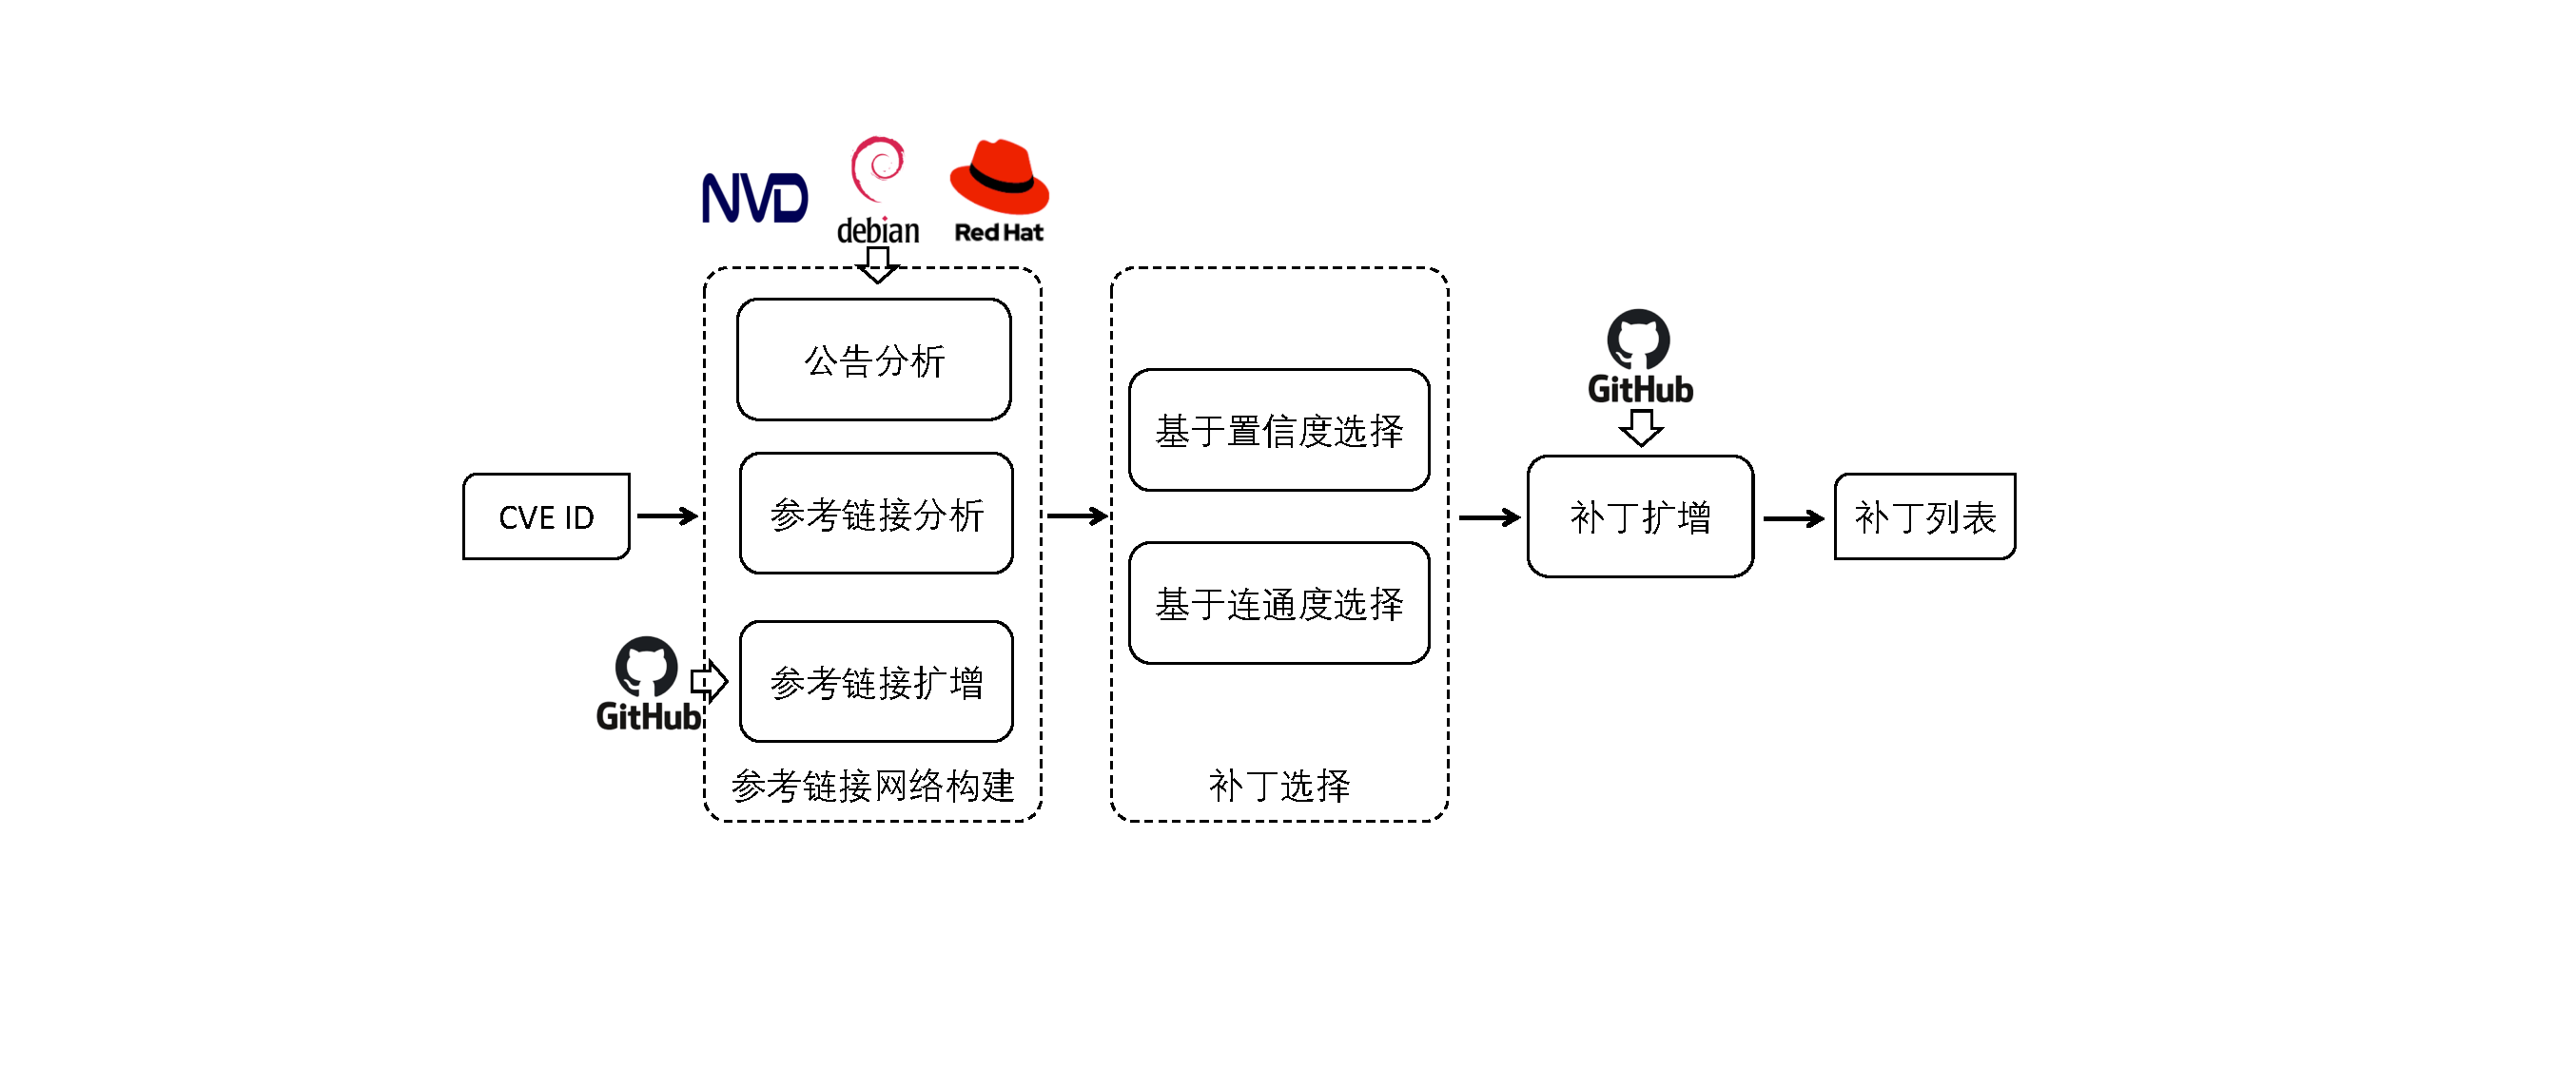
\includegraphics[scale=0.5]{fig/overview.pdf}
    %\vspace{-10pt}
    \caption{\tool 方法概览}\label{fig:overview}
\end{figure*}

基于前一章经验研究的发现,本文设计了一个名为\tool 的自动化开源软件漏洞的补丁识别方法。
该方法仅识别代码提交类型的补丁(即补丁提交,详见章节\ref{sec:type}),并构建一对多的漏洞补丁映射关系。该方法的核心思想是:漏洞的补丁会在与该漏洞相关的各种来源的漏洞公告、分析报告、讨论和解决的过程中被频繁地提及和引用。因此,本文首先设计了一种基于多知识源的漏洞参考链接网络,再从该网络中选出具有最高置信度和连通度的补丁节点作为结果,并基于选定的补丁构建一对多的漏洞补丁映射关系。

图\ref{fig:overview}为\tool 的方法概览。其中,\tool 以漏洞的CVE ID作为输入,主要经过三个步骤,最终返回补丁列表。步骤一,构建多源参考链接网络。该步骤的目的是将该漏洞在被报告、讨论和解决阶段引用的参考链接进行建模(参考链接,即引用的URL网址)。\tool 从多个\tocheck{漏洞知识源}(即NVD、Debian\footnote{https://security-tracker.debian.org/tracker/}、Red Hat\footnote{https://bugzilla.redhat.com/}和GitHub)中提取与该漏洞相关的参考链接并构建一个参考链接网络。这里将NVD视为主知识源,将Debian、Red Hat和GitHub视为次知识源,次级知识源列表可以不断扩增,以确保该方法的可扩展性和灵活性。步骤二,补丁选择。\tool 从构建的参考链接网络中选择中具有高连通性和高置信度的补丁节点作为该漏洞的补丁。步骤三,扩增补丁。经验研究中发现漏洞与其补丁之间存在一对多的映射关系。针对这一特征,基于步骤二中选定的补丁,\tool 通过搜索同一代码库所有分支中的相关代码提交来扩展补丁集。最终,\tool 返回该漏洞的补丁列表。
三个步骤的具体设计和实现将在下文中详细阐述。

% \begin{itemize}[leftmargin=*]
% \item 首先,\tool 从多个\tocheck{信息源}(即NVD、Debian\cite{debian}、RedHat\cite{redhat}和GitHub)为输入的CVE构建一个相关参考链接的网络。该步骤的目的是将CVE在报告、讨论和解决阶段的参考链接信息进行建模。这里将NVD视为主信息来源,将Debian、RedHat和GitHub视为次级信息来源,该级信息源可以进一步扩展。
% \item 其次,\tool 从构建的参考链接网络中,选择中具有高连通性和高置信度的补丁节点(即commit)作为该漏洞的补丁。
% \item 最后,\tool 通过搜索同一存储库中其他分支上的相关提交来扩展补丁集。该步骤目的是在CVE及其补丁之间建立潜在的一对多映射关系。
% \end{itemize}

\section{参考链接网络构建}
% \section{步骤一:构建多源参考链接网络}
\tool 的步骤一为漏洞参考链接网络构建,一共包括三个子步骤---公告分析、参考链接分析和参考链接扩增。前两个子步骤通过分析来自NVD、Debian和Red Hat三个知识源的漏洞公告及其中的参考链接,构建初始参考链接网络。第三个子步骤为从GitHub平台中搜索相关的代码提交,作为补丁节点扩入参考链接网络。

\subsection{公告分析} \label{sec:advisory analysis}
% 首先,\tool 初始化参考链接网络,将输入的CVE ID设置为根节点,获取三个漏洞知识源(即NVD、Debian和Red Hat)中该漏洞的公告,并将三个公告节点添加为根节点的子节点。这些公告节点便于后期追溯选定的补丁的信息来源。
输入CVE ID后,\tool 初始化参考链接网络,将输入的CVE ID设置为根节点,并将三个漏洞知识源(即NVD、Debian和Red Hat)中该漏洞的公告添加为根节点的子节点。这些公告节点可用于后期追溯补丁的来源。%(注:GitHub的引入将在章节\ref{}中介绍)

\begin{figure}[!t]
    \centering
    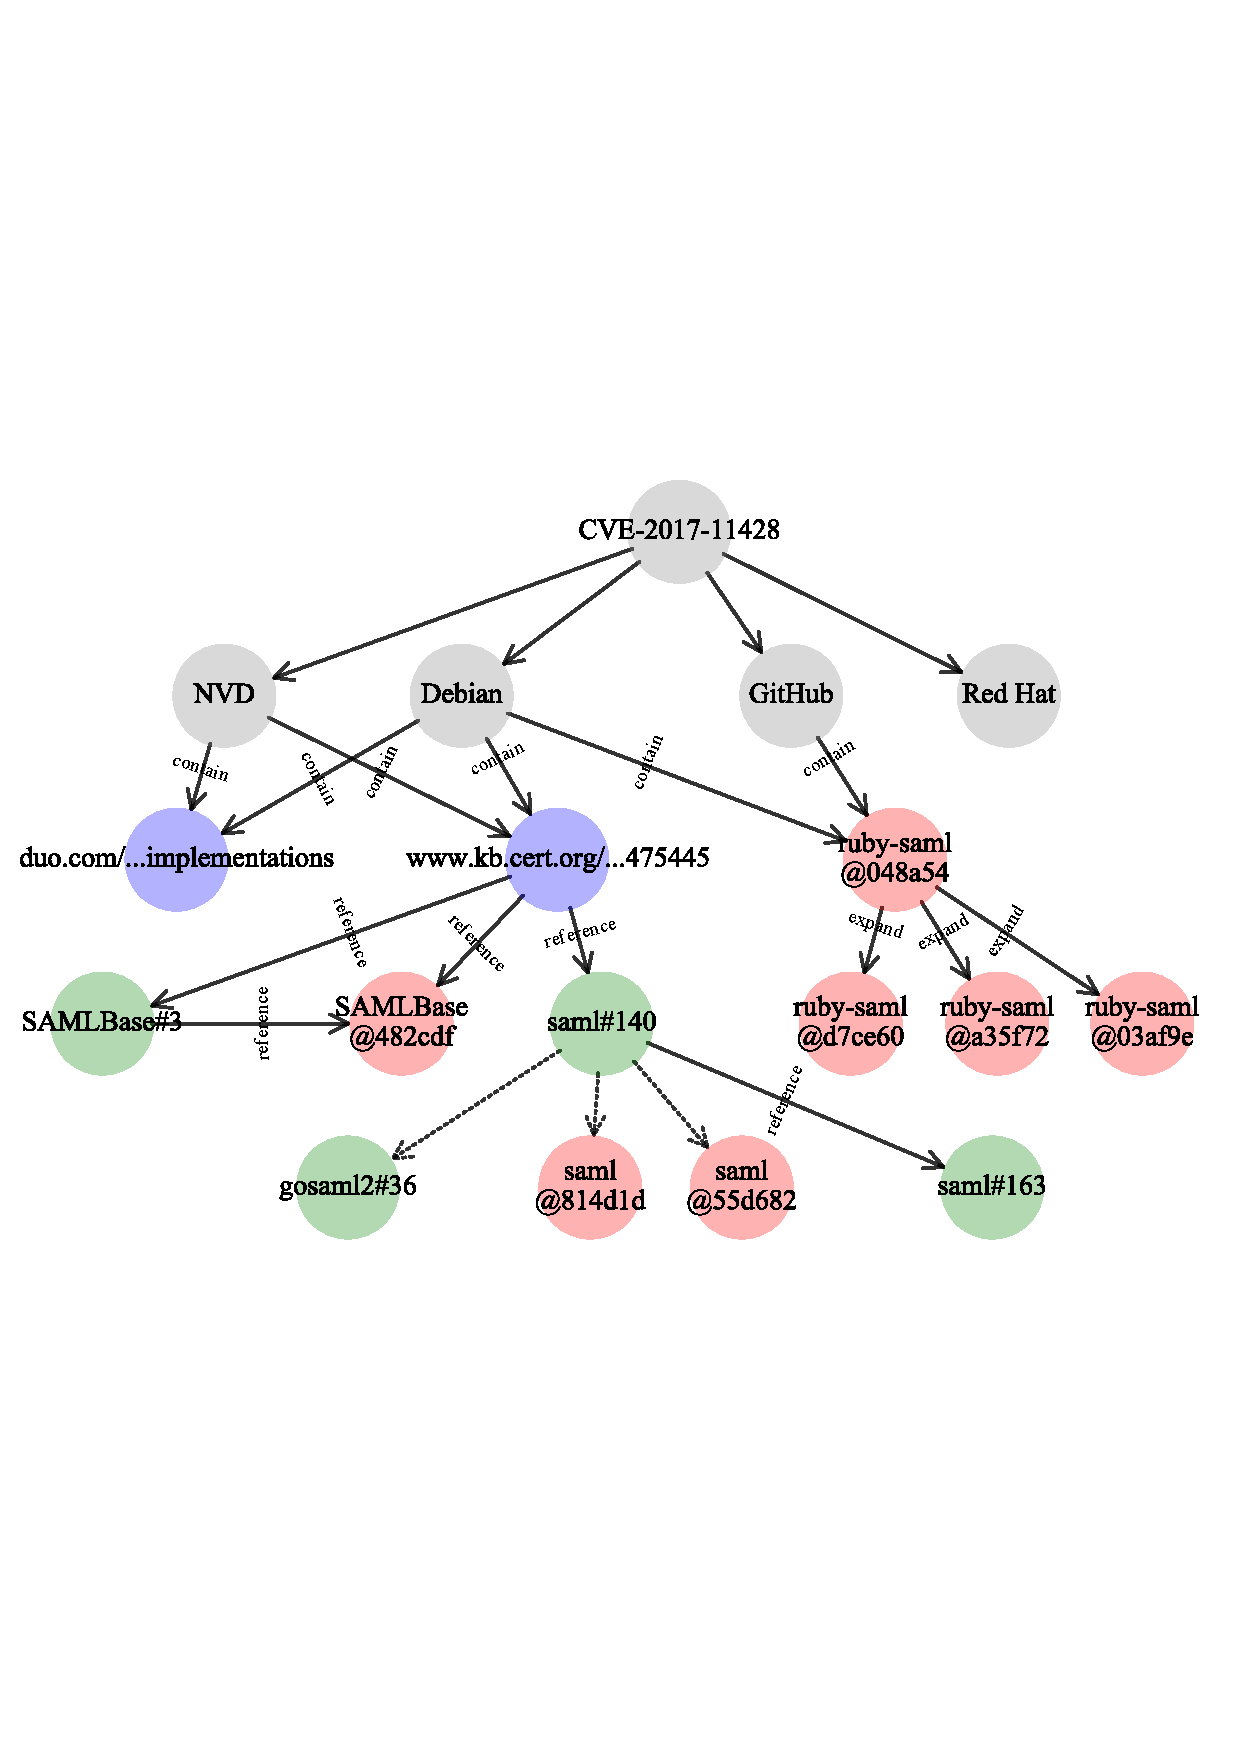
\includegraphics[scale=0.66]{fig/network-example.pdf}
    %\vspace{-10pt}
    \caption{漏洞CVE-2017-11428的多源参考链接网络}\label{fig:example}
\end{figure}

% \begin{table*}
%     \centering
%     \footnotesize
%     \caption{Temp  ref for Fig \ref{fig:An Example of toolname}}
%     \vspace{-10pt}
%     \begin{tabular}{|l|l|}
%     \noalign{\hrule height 1pt}
%     Identifier & URL\\\noalign{\hrule height 1pt}
%     N & https://nvd.nist.gov/vuln/detail/CVE-2017-11428\\
%     D & https://security-tracker.debian.org/tracker/CVE-2017-11428\\
%     R & https://bugzilla.redhat.com/show\_bug.cgi?id=CVE-2017-11428\\
%     ations & https://duo.com/blog/duo-finds-saml-vulnerabilities-affecting-multiple-implementations\\
%     475445 & https://www.kb.cert.org/vuls/id/475445\\
%     048a54 & https://nvd.nist.gov/vuln/detail/CVE-2017-11428\\
%     3 & https://github.com/Wizkunde/SAMLBase/issues/3\\
%     140 & https://github.com/crewjam/saml/pull/140\\
%     482cdf & https://github.com/onelogin/ruby-saml/commit/048a544730930f86e46804387a6b6fad50d8176f\\
%     d7ce60 & https://github.com/onelogin/ruby-saml/commit/d7ce607d9f9d996e1046dde09b675c3cf0c01280\\
%     a35f72 & https://github.com/onelogin/ruby-saml/commit/a35f7251b86aa3b7caf4a64d8a3451f925e8855c\\
%     03af9e & https://github.com/onelogin/ruby-saml/commit/03af9e33d2d87f4ac9a644c5b0981ded4dca0bb8\\
%     55d682 & https://github.com/crewjam/saml/commit/55d682de6bbefc17e979db16292f115467916919\\
%     814d1d & https://github.com/crewjam/saml/commit/814d1d9c18457deeda08cbda2d38f79bedccfa62\\
%     163 & https://github.com/crewjam/saml/issues/163\\
%     141 & https://github.com/crewjam/saml/pull/141\\
%     \noalign{\hrule height 1pt}
%     \end{tabular}
% \end{table*}

\begin{exmp}
图\ref{fig:example}为漏洞CVE-2017-11428\footnote{https://cve.mitre.org/cgi-bin/cvename.cgi?name=CVE-2017-11428}的多源参考链接网络。 其中,最顶层为根节点(即CVE ID),第二层为公告节点(即知识源NVD\footnote{https://nvd.nist.gov/vuln/detail/CVE-2017-11428}、Debian\footnote{https://security-tracker.debian.org/tracker/CVE-2017-11428}和Red Hat\footnote{https://bugzilla.redhat.com/show\_bug.cgi?id=CVE-2017-11428})。
\end{exmp}

然后,\tool 通过网络请求分别获取NVD、Debian和Red Hat平台中该漏洞的漏洞公告。NVD平台中,漏洞公告以JSON形式按年份存储于结构化数据\footnote{https://nvd.nist.gov/vuln/data-feeds}中,\tool 通过下载并解析相应的JSON文件即可获得NVD中该漏洞的公告信息。Debian平台中,漏洞公告也以结构化数据的形式存储在仓库\footnote{https://salsa.debian.org/security-tracker-team/security-tracker/-/tree/master/data/CVE}中,\tool 可直接从中解析得Debian提供的该漏洞公告信息。Red Hat平台提供了WebService API\footnote{https://bugzilla.redhat.com/docs/en/html/api/index.html}服务,\tool 可以直接使用该服务来检索Red Hat平台的漏洞公告。其中,Debian会跟踪NVD上的所有漏洞,而Red Hat仅跟踪NVD上的部分漏洞。

\tool 从每个知识源的漏洞公告中提取引用的参考链接信息,并将它们添加为相应公告节点的子节点。对于NVD公告,\tool 从“references”字段中直接获取取出相关参考链接。类似地,对于Debian公告,\tool 直接从“Notes”字段中提取出相关参考链接。对于Red Hat公告,\tool 使用正则表达式从评论区(“comments”字段)中提取出相关参考链接,这是因为开发人员常常会在评论区讨论和记录漏洞的解决过程并列出补丁,但NVD和Debian平台并无评论区模块。

\begin{figure}[!t]
    \centering
    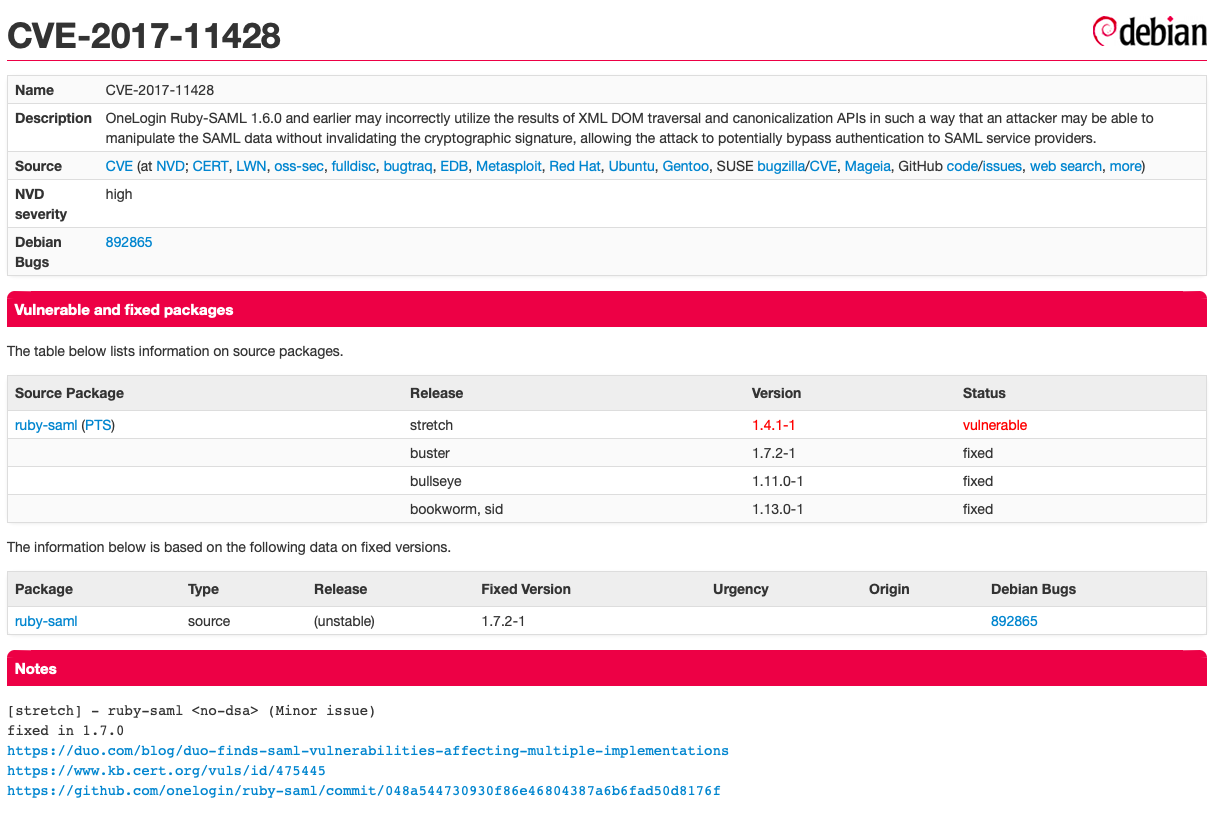
\includegraphics[scale=0.345]{fig/debian-2017-11428}
    %\vspace{-10pt}
    \caption{Debian平台中漏洞CVE-2017-11428的公告}\label{fig:debian-2017-11428}
\end{figure}

\begin{exmp}
如图\ref{fig:example}中的第三层所示,对于CVE-2017-11428,NVD公告中包含了两个参考链接。链接一\footnote{https://duo.com/blog/duo-finds-saml-vulnerabilities-affecting-multiple-implementations}是对描述此漏洞细节的博客的引用,链接二\footnote{https://www.kb.cert.org/vuls/id/475445}是对该漏洞的第三方公告的引用。如图\ref{fig:debian-2017-11428}所示,这两个参考链接也包含在Debian公告中,不过Debian公告还包含修复此漏洞的GitHub提交链接ruby-saml@048a54\footnote{https://github.com/onelogin/ruby-saml/commit/048a544730930f86e46804387a6b6fad50d8176f}。此外,Red Hat平台并未收录该漏洞,所以也无参考链接信息。
\end{exmp}

基于参考链接网页的内容,\tool 将参考链接节点分为三种类型:补丁节点(Patch Node)、\tocheck{问题节点}(Issue Node)和\tocheck{混合节点}(Hybrid Node)。这里区分出补丁节点,是因为该方法的根本目的就是在多个知识源中找到所引用的补丁。识别补丁节点的方法为,如果参考链接中包含“git”字段且可通过正则表达式匹配到代码提交ID(Commit ID),则该链接为Git提交形式的补丁节点;如果参考链接中包含“svn”字段且可通过正则表达式匹配到代码提交ID(Commit ID),则该链接为SVN提交形式的补丁节点。

这是还区分出问题节点,是因为开发人员常常会在问题追踪系统(Issue Tracker)中为漏洞申请一个问题报告(Issue Report,也称为工单),并在该报告的评论区讨论解决方案并引用补丁链接。所以,问题报告是一种较为特殊且重要的参考链接。此外,问题追踪系统中的问题报告会有一个问题标识符(Issue ID),开发人员常常会将此问题标识符写入代码提交信息(Commit Message)中。有利于识别漏洞相关的代码提交,详见章节\ref{sec:addGithub}。识别问题节点的方法为,如果参考链接中包含“/github.com/”和“/issues/”,则该链接为GitHub Issue类型的问题节点。如果参考链接中包含“/github.com/”和“/pull/”,则该链接为GitHub抓取(Pull Request)类型的问题节点。如果参考链接中包含“bugzilla”、“jira”、“issues”、“bugs”、“tickets”和“tracker”中的某一个字段且可通过正则表达式匹配到问题标识符(Issue ID),则该链接为通用类型的问题节点。对于所有未识别为补丁或问题节点的参考链接信息将被视为混合节点,它们多为博客、第三方漏洞公告等。

%受经验研究中补丁类型分析结果启发(Sec.\ref{sec:type}),

\begin{exmp}
如图\ref{fig:example}中的第三层所示,NVD和Debian公告中包含的两个参考链接被标识为混合节点(即图中的两个紫色节点),仅有一个在Debian公告中的参考链接被识别为补丁节点(即图中的红色节点)。该漏洞在该步骤中未识别到问题类型节点。
\end{exmp}

\subsection{参考链接分析}
对于前序步骤中已添加入图的每个参考链接节点,\tool 将通过以下两种节点分析方式,以分层迭代的方式继续扩建参考链接网络。%\tool 将通过“引用分析”和“信息增强”两个步骤以分层方式继续构建参考链接网络。

\textbf{方式一,}如果该参考链接节点的类型为补丁节点,\tool 会通过网络请求该代码提交的内容并分析该代码提交是否只涉及了测试代码或非代码文件的修改。如果是的话,则表明该代码提交一定不是用于修复漏洞的补丁提交,\tool 会从网络中删除该节点。对于测试代码的判定,\tool 通过检查修改的文件路径中是否含有“test”字段来判断,如果文件路径含有“test”字段则判定为测试文件。对于源代码文件的判定,\tool 通过检查修改文件的后缀来识别该文件是否为代码文件,如果文件的后缀非常见代码文件类型,即不在列表\footnote{常见代码文件后缀列表:['java', 'py', 'c', 'cc', 'cpp', 'cxx', 'c++', 'js', 'go', 'rb', 'cs', 'as', 'php', 'pl', 'coffee', 'h', 'm', 'ts', 'kt', 'mjs', 'twig', 'htaccess', 'tpl', 'pt', 'scala', 's', 'erb', 'swf', 'asm', 'groovy', 'jsp', 'sh', 'hpp', 'phps', 'script', 'wscript', 'ldif', 'Tokens', 'nsi', 'tcl', 'idl', 'pyx', 'ps1', 'toml', 'inl', 'x', 'S', 'hbs']}中则判定为非源代码文件。

\textbf{方式二,}如果该参考链接节点的类型为问题节点或混合节点,\tool 会通过网络请求该参考链接的页面信息(即HTML文本),并解析出该网页中引用的参考链接,将其作为子节点扩入参考链接网络。首先,对于网页中参考链接的提取,\tool 使用正则表达式提取纯文本中的URL,同时使用HTML解析器提取超链接(即\textbf{<a>}标签)中的URL。
然后,使用章节(\ref{sec:advisory analysis})中相同的方式识别参考链接类型,并将这些引用添加为当前节点的子节点。值得注意的是,在该步骤及以后流程中参考链接网络将不再加入混合节点。这是因为混合节点极易引入噪声,随着网络构建得越深,噪声也就越多。所以,除了直接被NVD、Debian和Red Hat公告节点引用的混合节点,其他参考链接节点分析中将不再考虑混合节点,仅识别补丁节点和问题节点。此外,考虑到GitHub Issue中通常会引用来自其他软件仓库的问题或提交的链接,这给网络带来过多的噪音且使网络空间爆炸。因此,在该步骤中,如果被分析的参考链接节点为GitHub Issue类型,则仅仅将该节点引用的同一代码仓库中的代码提交或问题节点添加到网络中。

对于所有新增的节点,\tool 将一直重复以上两种节点分析的方式迭代扩增网络,直到没有任何新增的节点或者网络深度达到设定的阈值(网络深度默认为\tocheck{5}层),该步骤结束。

\begin{figure}[!t]
    \centering
    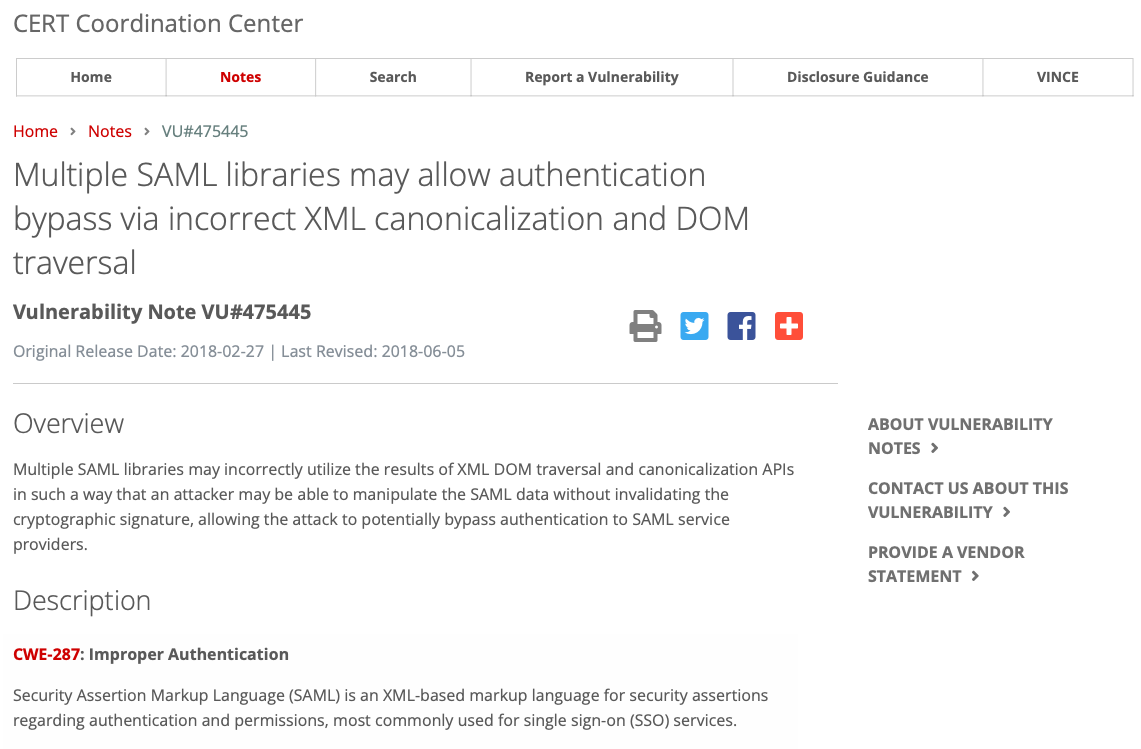
\includegraphics[scale=0.35]{fig/457445-0}
    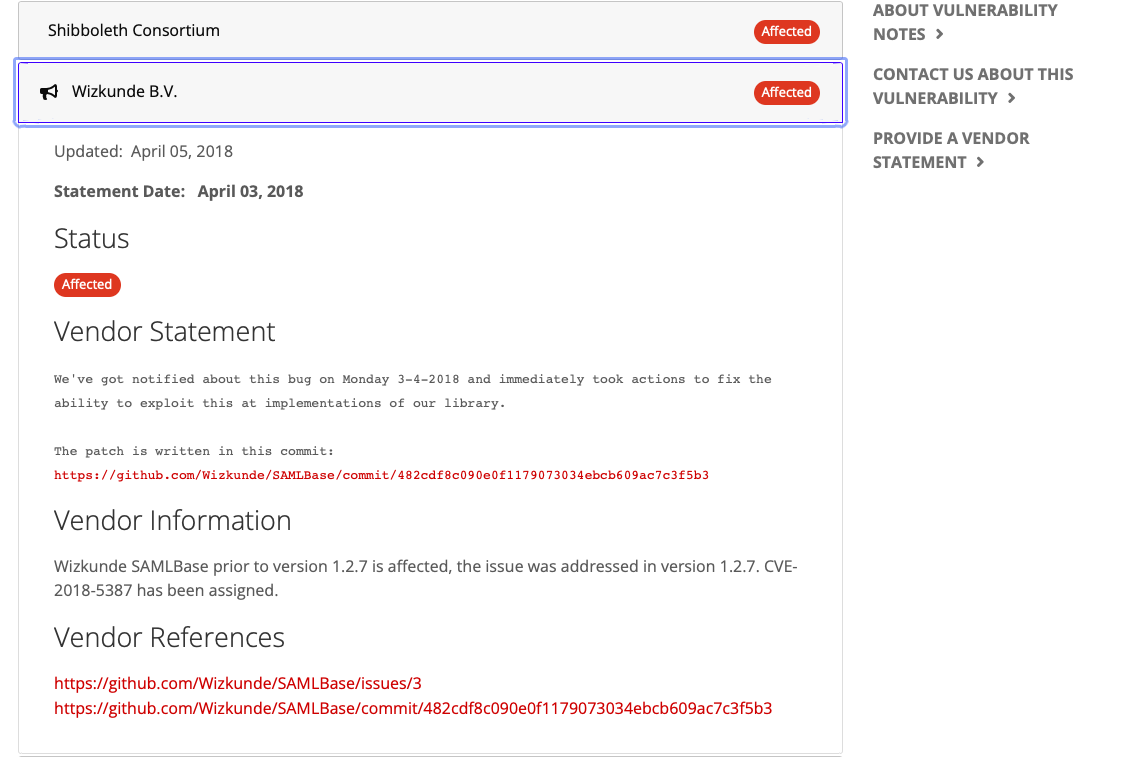
\includegraphics[scale=0.35]{fig/457445-1}
    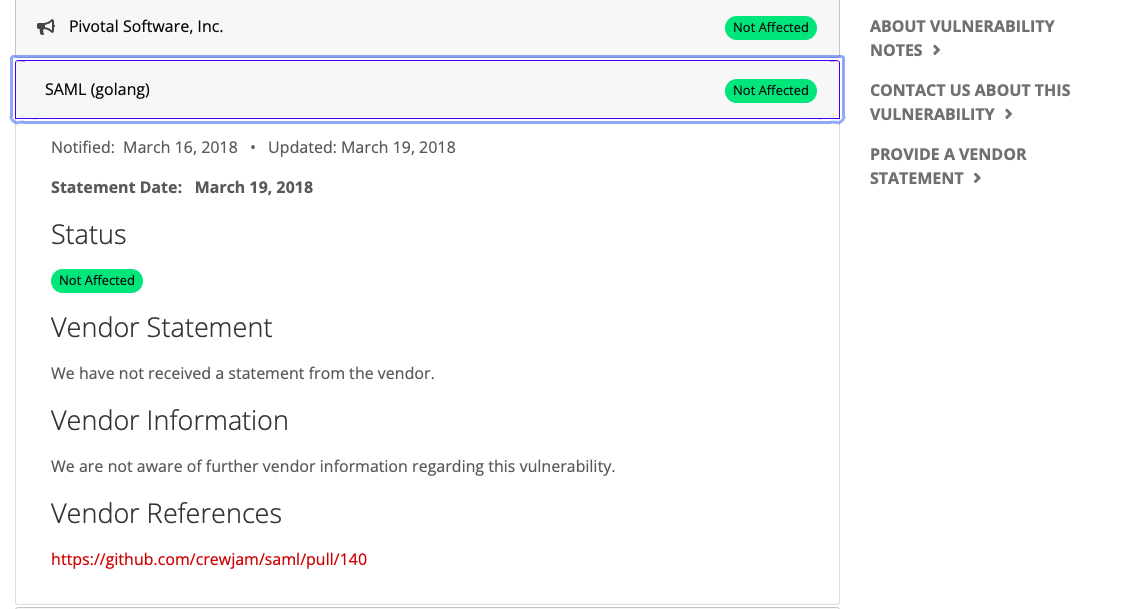
\includegraphics[scale=0.35]{fig/457445-2}
    %\vspace{-10pt}
    \caption{混合节点“www.kb.cert.org/...475445”}\label{fig:457445}
\end{figure}

\begin{exmp}
在第一次迭代中,因为ruby-saml@048a54并非仅涉及测试代码或非源代码文件的更改,所以\tool 将补丁节点ruby-saml@048a54保留在图\ref{fig:example}中第三层。此外,\tool 标识还出第三层中的两个混合节点,其中一个混合节点未引用任何问题或提交链接,另一个混合节点了引用了两个问题链接SAMLBase\#3和saml\#140以及一个代码提交链接SAMLBase@482cdf。图\ref{fig:457445}为混合节点“www.kb.cert.org/...475445”引用的代码提交SAMLBase@482cdf\footnote{https://github.com/GoGentoOSS/SAMLBase/commit/482cdf8c090e0f1179073034ebcb609ac7c3f5b3}、问题链接SAMLBase\#3\footnote{https://github.com/GoGentoOSS/SAMLBase/issues/3}和问题链接saml\#140\footnote{https://github.com/crewjam/saml/pull/140}。

在第二次迭代中,\tool 发现节点SAMLBase\#3引用了SAMLBase@482cdf,而节点saml\#140引用了两个问题链接gosaml2\#36和saml\#163以及两个代码提交链接saml@814d1d和saml@55d682。考虑到gosaml2\#36与saml\#140并不属于同个代码仓库,saml@814d1d和saml@55d682也仅涉及测试代码的更改,\tool 便不将它们添加到网络中。为了便于示例讲解,这些未添加的节点仍显示在图\ref{fig:example}中,但以虚线连接。图\ref{fig:814d1d9}为代码提交链接saml@814d1d\footnote{https://github.com/crewjam/saml/commit/814d1d9c18457deeda08cbda2d38f79bedccfa62},可以发现,该提交仅修改了“service\_provider\_test.go”一个文件,且该文件为测试代码文件。
%在此迭代之后,达到深度限制。
\end{exmp}

\begin{figure}[!t]
    \centering
    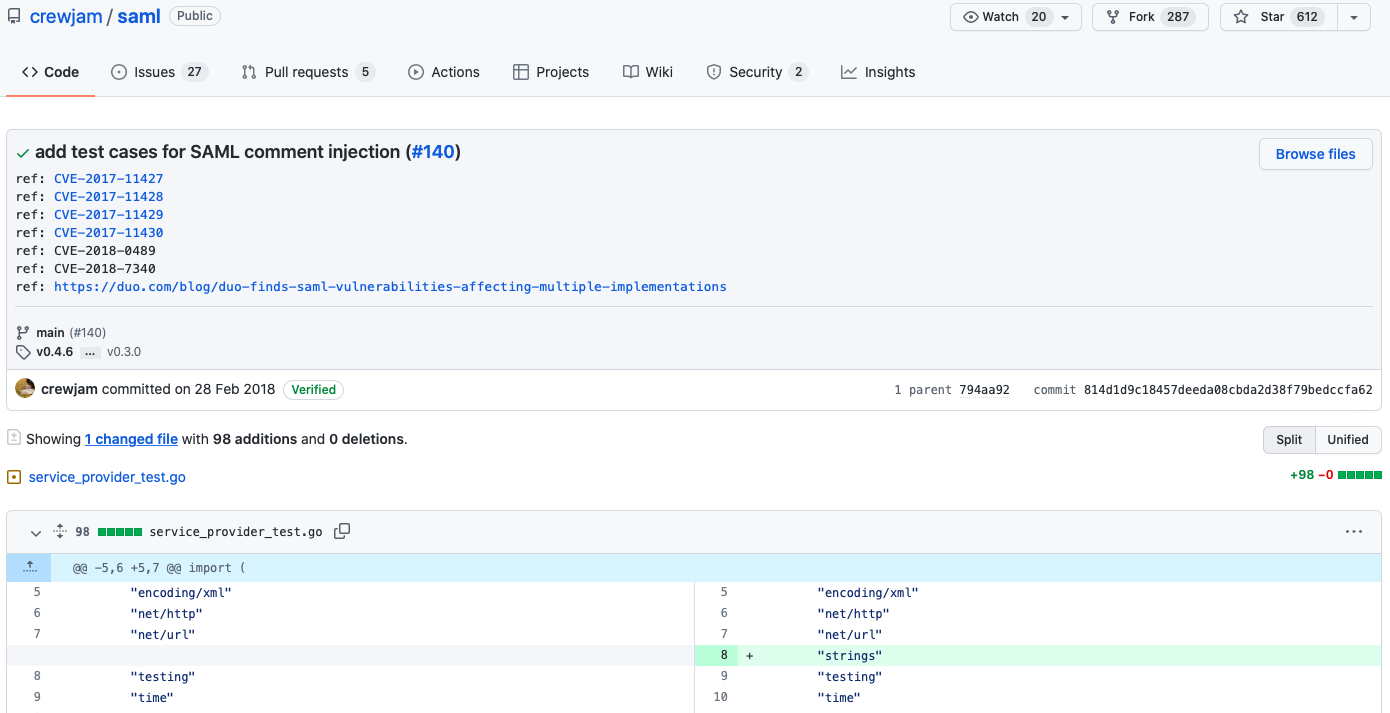
\includegraphics[scale=0.29]{fig/commit-814d1d9}
    %\vspace{-10pt}
    \caption{“saml@814d1d”代码提交}\label{fig:814d1d9}
\end{figure}

\subsection{参考链接扩增}\label{sec:addGithub}
除了NVD、Debian和Red Hat等漏洞公告平台可作为漏洞知识来源之外,代码托管平台也可以被视为隐含的知识来源,因为补丁通常隐藏在代码仓的代码提交历史中。因此,在该步骤中,\tool 将搜索代码托管平台以获取漏洞的补丁提交,并将检索到的补丁扩增到该漏洞的参考链接网络。

受经验研究中补丁类型分析结果的启发,93.7\%的补丁都为GitHub代码提交的形式(见章节\ref{sec:type}),所以在该步骤中\tool 只搜索GitHub平台的代码提交。此外,问题跟踪系统通常还会为漏洞相关的问题分配一个问题标识符(Issue ID)。同样,软件厂商通常也会为该漏洞分配一个漏洞公告标识符(Advisory ID)。例如,受漏洞CVE-2019-10426影响的软件厂商为漏洞分配的标识符为SECURITY-1573\footnote{https://www.jenkins.io/security/advisory/2019-09-25/\#SECURITY-1573},问题跟踪系统为该漏洞分配的问题标识符为THRIFT-4647\footnote{https://issues.apache.org/jira/browse/THRIFT-4647}。这些标识符会包含在修复补丁的代码提交中。针对这一特征,\tool 使用正则表达式从已有的网络节点中分别提取问题标识符和公告标识符,并与漏洞标识符一起作为关键词,检索GitHub中的代码提交。

\tool 通过GitHub提供的REST API\footnote{https://docs.github.com/en/rest/reference/search\#search-commits}接口,全站搜索GitHub中相关的代码提交。%针对一次搜索,该API最多返回 1,000个搜索结果。
为了减少噪音,对于API返回的提交,\tool 首先会检查该代码提交的仓库信息是否与漏洞的CPE\footnote{https://nvd.nist.gov/products/cpe}信息匹配。其中,CPE是针对受漏洞影响软件的结构化命名方案,包括供应商和产品名称信息,可以直接从NVD的JSON文件中解析得到。
对于代码提交的仓库信息与CPE信息匹配的判定,\tool 沿用了Dong 等人的匹配准则\cite{dong2019towards},该准则可灵活地应对同一个软件名称存在不同别名的情况。具体来说,给定两个软件的名称,如果匹配的单词数不小于不匹配的单词数,则这两个软件的名称匹配成功,视为同一软件。此外,\tool 仍会检查该提交是否为测试代码或非代码文件的更改。如果这两个检查都通过,\tool 会将其作为GitHub节点的子节点加入网络。

\begin{figure}[!t]
    \centering
    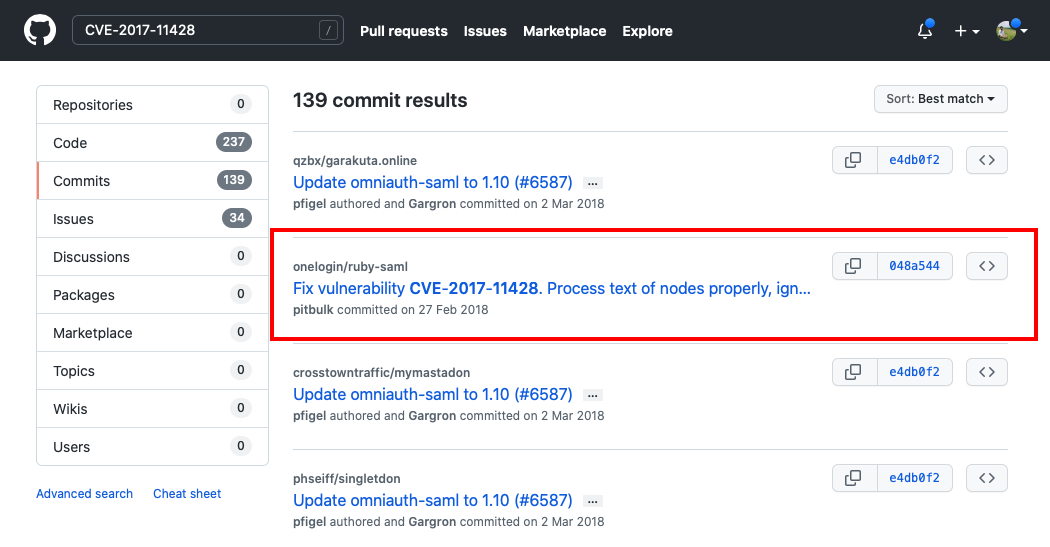
\includegraphics[scale=0.39]{fig/commit-048a54}
    %\vspace{-10pt}
    \caption{关键词“CVE-2017-11428”的搜索结果}\label{fig:048a54}
\end{figure}

\begin{exmp}
对于样例CVE-2017-11428,\tool 无法从构建的网络中提取任何问题或公告标识符。因此,\tool 仅使用CVE标识符(CVE ID)来搜索GitHub中相关的代码提交。如图\ref{fig:048a54}所示,搜索返回的提交有ruby-saml@048a54,其仓库信息是“onelogin: ruby-saml”;此CVE-2017-11428的CPE是“onelogin: ruby-saml”,因此实现了名称的完全匹配,\tool 将会把ruby-saml@048a54节点加入网络。由于该节点已包含在参考网络中,\tool 便不再新增节点,将其连接为GitHub节点的子节点,见图\ref{fig:example}。此外,该次搜索结果中没有其他匹配的代码提交。
\end{exmp}   

\section{补丁选择}\label{sec:selection}

步骤二的设计目标是尽可能准确且完整地从该漏洞参考链接网络中选择出补丁节点。为了实现这一目标,本小节设计了以下两种补丁选择方法。

\subsection{基于置信度的补丁选择方法}
在该方法中,\tool 将直接选择具有高置信度的补丁作为正确的补丁。具体来说,本文认为参考链接网络中的两种补丁节点具有比较高的置信度。

第一种,为被NVD直接引用的补丁节点,即图中作为NVD子节点的补丁节点,被认为具有高置信度。这是因为NVD数据库建立在强大的社区支持下,每个漏洞的信息都经过多个流程的人工确认,且初始漏洞报告在发布后还会不断维护更新。因此,本文认为NVD中的补丁具有较高的精度。此外,已有的很多工作\cite{duan2019automating, li2016vulpecker, li2018vuldeepecker}都是基于这种方法来查找补丁。

第二种,为从Github直接搜索出的补丁节点,即图中作为GitHub子节点的补丁节点,被认为具有高置信度。这是因为在将此类补丁节点添加到网络前,经过了较为严苛的确认。\tool 会确保代码提交信息中包含该漏洞的CVE ID、 Advisory ID或Issue ID,并且其所属的仓库信息必须与该漏洞的CPE名称成功匹配。这种方法也在已有的很多工作\cite{you2017semfuzz, Wang2020empirical}中使用。

\begin{exmp}
在漏洞CVE-2017-11428的参考链接网络中(图\ref{fig:example}),\tool 将直接选择补丁节点ruby-saml@048a54作为补丁结果之一。因为该节点是GitHub节点的子节点,具有较高的置信度。实际上,ruby-saml@048a54也确实是正确的补丁之一。
\end{exmp}

\subsection{基于连通度的补丁选择方法}
仅仅使用基于置信度的启发式方法通常不足以完整地找出漏洞补丁集。因为NVD中很可能不包含补丁链接,且CVE ID、 Advisory ID或Issue ID也很可能不在代码提交信息中,因此也无法通过搜索Github获取到补丁。考虑到漏洞的补丁会在与该漏洞相关的各种来源的漏洞公告、分析报告、讨论和解决的过程中被频繁提及和引用,这也意味着:正确的补丁节点将会广泛地连接到网络中的根节点(即图中的CVE ID节点)上。因此,本文还设计了基于连通度的补丁节点选择方法。

具体来说,\tool 从两个角度衡量网络中补丁节点与根节点间的连通度。一是路径数,根节点可到达补丁节点的路径越多,补丁节点与根节点的连通性就越高;二是路径长度,从根节点到补丁节点的路径越短,补丁节点到根节点的连通性就越高。为了结合这两个方面,\tool 使用公式\ref{eq:connectivity}计算补丁节点到根节点的连通度。其中,$ p = 1, ..., n$表示从根节点到补丁节点的$n$条路径,$d_p$表示路径$p$的长度。考虑到NVD和GitHub子节点的高置信度,如果路径$p$源于NVD和GitHub节点,则路径长度自动减1。

\begin{equation}\label{eq:connectivity}
    connectivity =\sum_{p=1}^{n}   \frac{1}{2^{({d}_{p} -1)}}
\end{equation}

基于每个补丁节点到根节点的连通度,\tool 选择连通度最高的节点作为该漏洞的补丁,加入补丁集。

\begin{exmp}
在图\ref{fig:example}中,从根节点到补丁节点ruby-saml@048a54的路径有两条。一是源自Debian的路径,长度为2,连通度为0.5。另一个是源自GitHub的路径,原始长度为2,调整后为1,连通度为1。因此,ruby-saml@048a54节点到根节点的总连通度为1.5。同理,从根节点到补丁节点SAMLBase@482cdf存在四条路径,连通性分别为0.5、0.25、0.25和0.125。因此,SAMLBase@482cdf到根节点的连通度为1.125,低于ruby-saml@048a54节点,所以\tool 选择ruby-saml@048a54作为补丁。%,因为它具有最高的连接性。
  %\tool 选择它作为 CVE-2017-11428 的补丁。
\end{exmp}

完成以上两种补丁选择方法后,\tool 已从该漏洞的参考链接网络中选出补丁集。由于构建该网络的过程中可能没有识别到补丁链接,所以该补丁集可能为空。同时,基于以上两种补丁选择方法,\tool 也有可能已获得该漏洞的多个补丁。


\section{补丁扩增}
受经验研究中映射分析结果的启发,漏洞其补丁之间存在一对多的映射关系。章节\ref{sec:cardinality}中,映射分析结果表明,超过\tocheck{40\%}的漏洞与其补丁具有一对多的映射关系,且这些补丁通常是位于同一代码库的某一个或多个分支。对于这种多补丁的漏洞,\tool 在前两个步骤中构建的网络无法确保能完整地包含所有补丁。针对这一情况,基于步骤二中选出的补丁,步骤三通过搜索同一代码库所有分支中的相关提交来扩展补丁集。此外,补丁类型分析(Sec.\ref{sec:type})表明绝大多数的补丁都以GitHub代码提交的形式。因此,\tool 的步骤三具体设计如下:对于每个已在步骤二中选定的GitHub代码提交形式的补丁,\tool 将首先获取其Github代码仓库信息,并获取该仓库中的所有分支信息,在每个分支的特定时间范围内搜索相关的代码提交。

具体来说,对于GitHub代码提交形式的补丁,\tool 从补丁链接中提取出仓库信息,即所有者(Owner)和存储库(Repository)信息。基于补丁提交的所有者和仓库名信息,\tool 先使用GitHub的REST API\footnote{https://docs.github.com/en/rest/reference/repos\#list-branches}获取存储库中的所有分支信息。对于每个分支,\tool 再通过GitHub的REST API\footnote{https://docs.github.com/en/rest/reference/repos\#list-commits}检索选定补丁之前和之后特定时间跨度内的提交,时间跨度默认为\tocheck{30天}。这里设置时间跨度,是考虑到工具时间性能和准确性之间的平衡。当项目历史较长且不设置时间限制时,\tool 运行时长也会无限增长。

然后,对于API返回的特定时间跨度内的提交,\tool 使用以下两个标准来确定该提交是否与选定补丁具有相关性:一是提交信息(Commit Message)与已选补丁的提交消息相同或是包含关系;二是提交消息包含CVE ID、 Advisory ID或Issue ID。如果检索返回的提交满足这两个条件之一,\tool 会将该补丁扩展为选定补丁的子节点。

最后,\tool 将返回步骤二中选定的补丁和步骤三中扩展的补丁作为补丁列表返回给用户。此外,\tool 还返回该漏洞的参考链接网络,以便于工作人员追溯补丁的来源及关系。%,从补丁集选定确认正确的补丁。

\begin{figure}[!t]
    \centering
    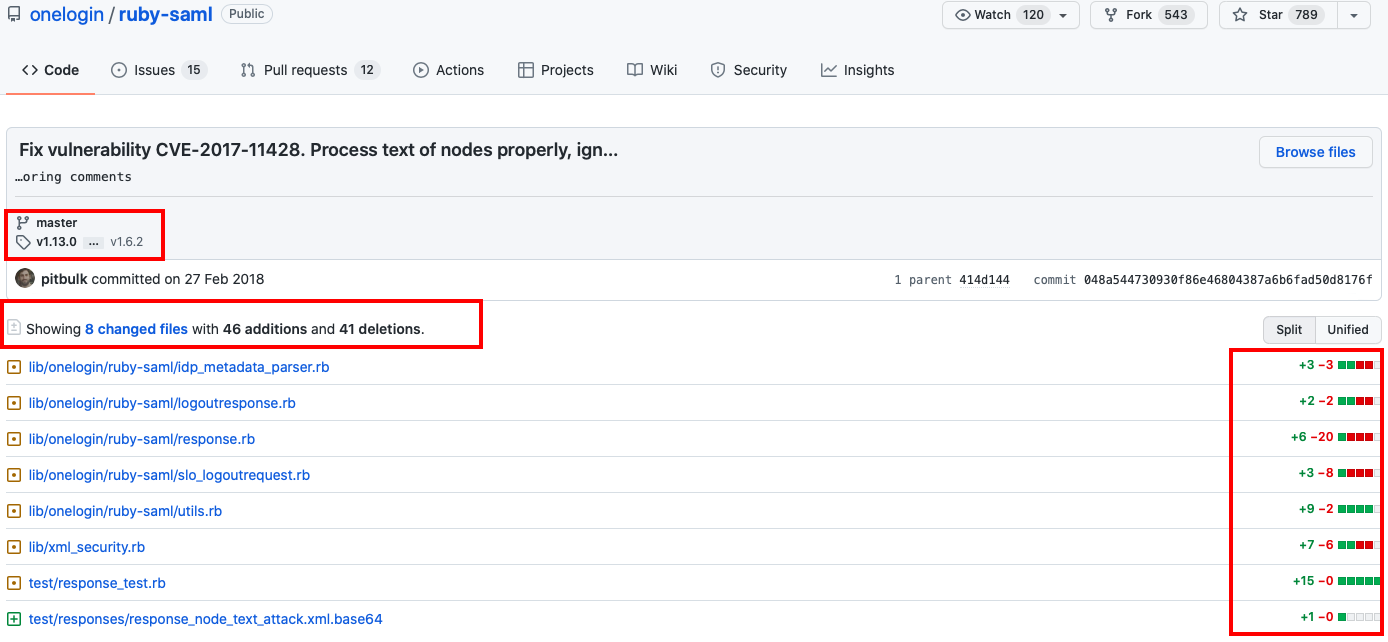
\includegraphics[scale=0.30]{fig/11428-commit-048a54}
    % \vspace{-10pt}
    \caption{“ruby-saml@048a54”代码提交}\label{fig:048a54}
\end{figure}

\begin{figure}[!t]
    \centering
    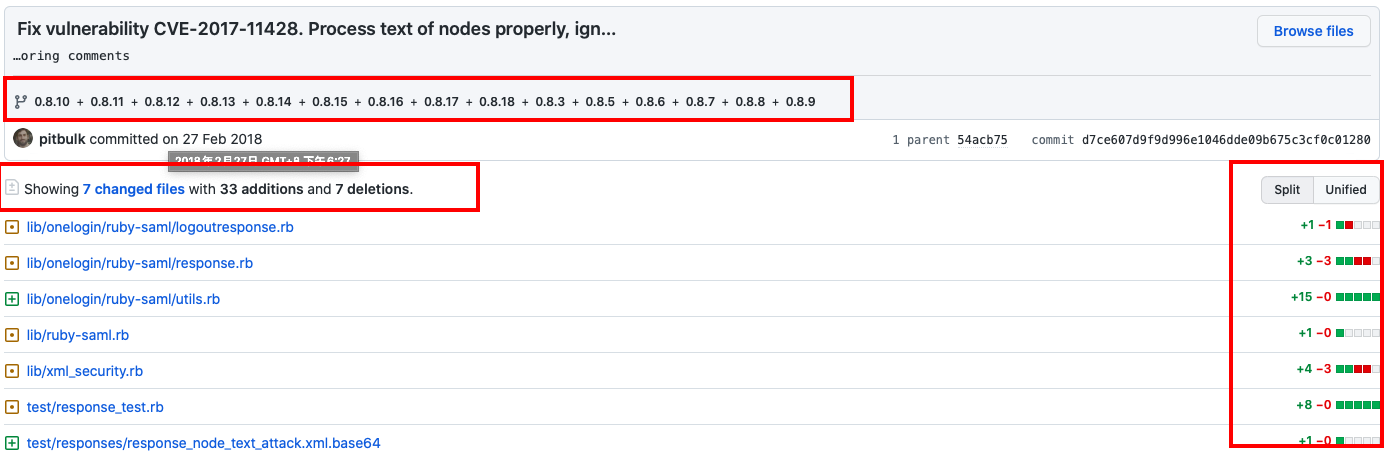
\includegraphics[scale=0.30]{fig/11428-commit-d7ce60}
    % \vspace{-10pt}
    \caption{“ruby-saml@d7ce60”代码提交}\label{fig:d7ce60}
\end{figure}

\begin{figure}[!t]
    \centering
    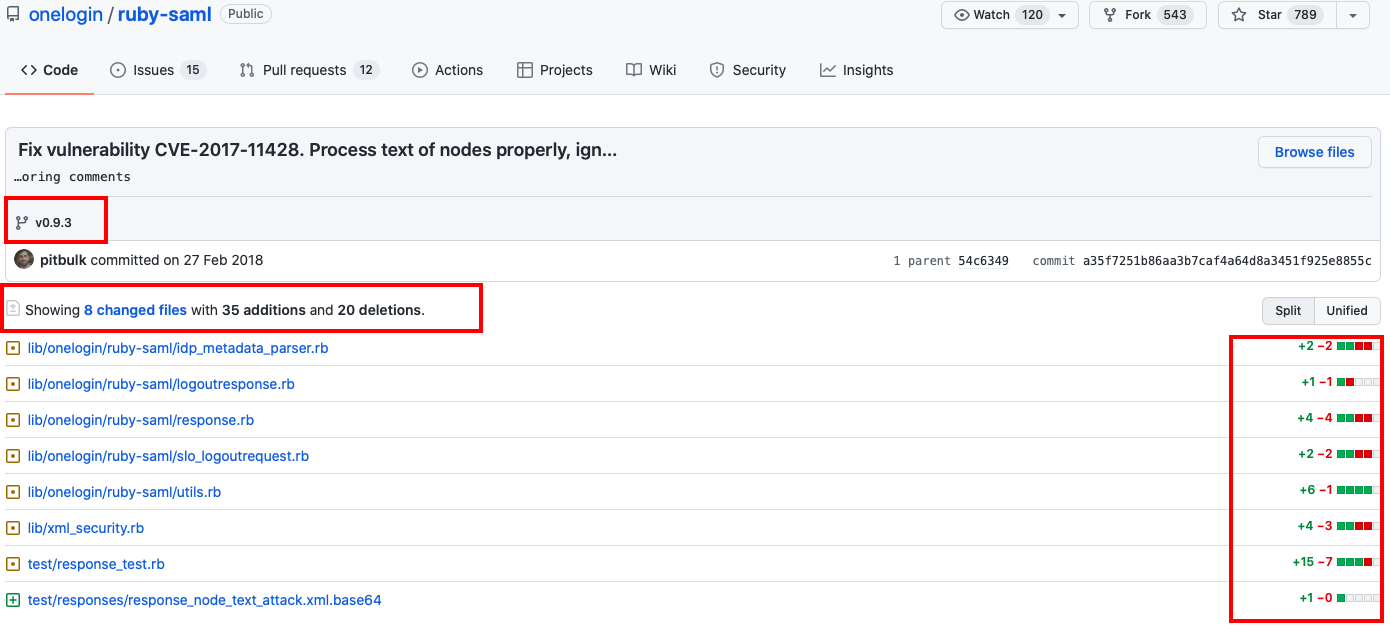
\includegraphics[scale=0.30]{fig/11428-commit-a35f72}
    % \vspace{-10pt}
    \caption{“ruby-saml@a35f72”代码提交}\label{fig:a35f72}
\end{figure}

\begin{figure}[!t]
    \centering
    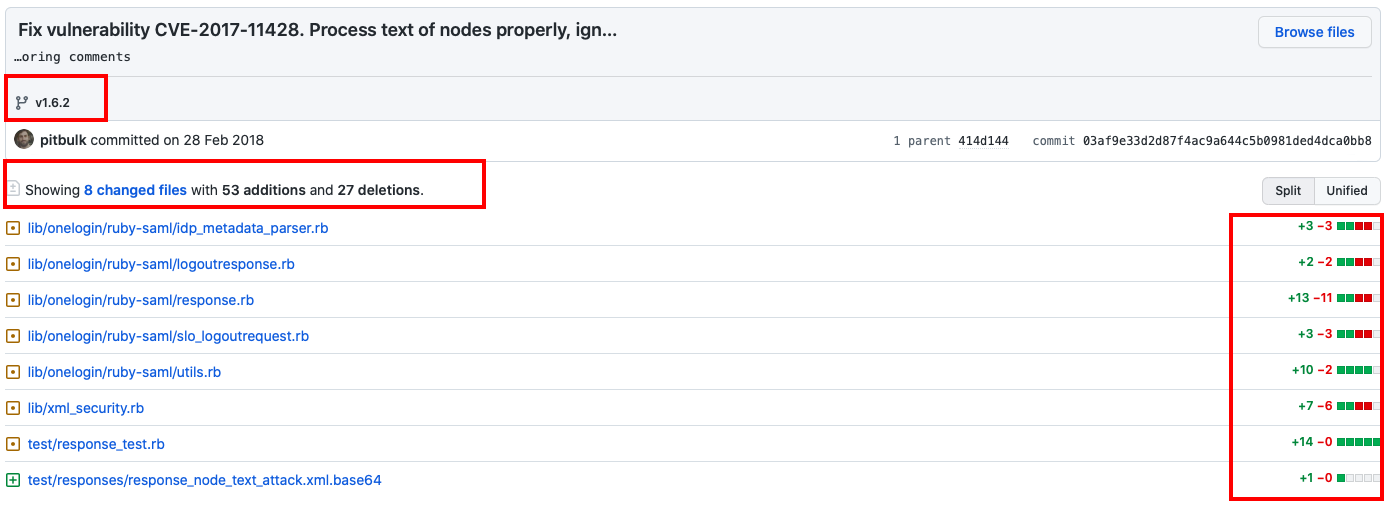
\includegraphics[scale=0.30]{fig/11428-commit-03af9e}
    % \vspace{-10pt}
    \caption{“ruby-saml@03af9e”代码提交}\label{fig:03af9e}
\end{figure}

\begin{exmp}
在步骤二中,\tool 为漏洞CVE-2017-11428选出的补丁为ruby-saml@\\048a54(位于主分支)。在步骤三种,\tool 查找到了另外三个提交---ruby-saml@d7ce60\footnote{https://github.com/onelogin/ruby-saml/commit/d7ce607d9f9d996e1046dde09b675c3cf0c01280}、ruby-saml@a35f72\footnote{https://github.com/onelogin/ruby-saml/commit/a35f7251b86aa3b7caf4a64d8a3451f925e8855c}和ruby-saml@03af9e\footnote{https://github.com/onelogin/ruby-saml/commit/03af9e33d2d87f4ac9a644c5b0981ded4dca0bb8}。图\ref{fig:048a54}、\ref{fig:d7ce60}、\ref{fig:a35f72}和\ref{fig:03af9e}所示,它们与选定补丁ruby-saml@048a54具有相同的提交信息却不同的代码更改。这三个提交分别位于分支0.8.3--0.8.17、v0.9.3和v1.6.2中。如图\ref{fig:example}所示,\tool 将三个提交添加为ruby-saml@048a54的子节点。实际上,这四个代码提交也确实都是CVE-2017-11428的正确补丁,而数据库$DB_A$和$DB_B$都只提供了ruby-saml@048a54一个补丁。
\end{exmp}
\chapter{实验评估}

本章将详细阐述为评估\tool 所进行的实验验证,并讨论分析实验的结果。本章将首先介绍所设计的五个实验问题,包括准确性、削弱性、敏感度、通用性及实用性的验证;再逐一展示五个问题的实验结果,并讨论分析其原因及意义;最后,基于实验验证的结果,讨论\tool 的局限性以及实际价值。

\section{实验问题设计}
本文从准确性、削弱性、敏感度、通用性及实用性五个方面设计了以下五个研究问题,以尽可能全面地验证并评估\tool 。

\begin{itemize}[leftmargin=*]
\item \textbf{RQ6 准确性评估:}与已有的基于启发式的方法相比,\tool 查找漏洞补丁的准确性如何?与两个商业漏洞数据库相比,\tool 提供的漏洞补丁的准确性又如何呢?这个问题旨在探究\tool 的准确性。(见章节\ref{sec:accuracy-evaluation})
\item \textbf{RQ7 削弱性分析:}\tool 中各个步骤及设计有着怎么样的效果或必要性?如果去除或削弱\tool 中的某些环节,对于\tool 的结果会有怎么样的影响?这个问题旨在评估\tool 中各个步骤及设计的实际效果及必要性。(Sec.\ref{sec:ablation})
\item \textbf{RQ8 敏感度分析:}\tool 的准确性对\tool 中参数的敏感性如何?这个问题旨在评估\tool 的健壮性及鲁棒性,探究tool 中的参数是否对\tool 的准确性有过大影响。 (见章节\ref{sec:sensitivity})
\item \textbf{RQ9 通用性分析:}\tool 在更大范围的开源软件漏洞上表现如何? 这个问题旨在评估\tool 的通用性。(见章节\ref{sec:sensitivity})
\item \textbf{RQ10 实用性分析:}\tool 在实际使用中表现如何?这个问题旨在评估\tool 在实际使用中实用性。(见章节\ref{sec:generality})
\end{itemize}

为解答以上实验问题,本章的实验验证将继续采用经验研究(见章节\ref{sec:accuracy})中使用的评估指标,即Not Found、Precision(精确率)、Recall(召回率)和 F1-Score(F1值)。本章的实验验证还将继续使用在经验研究(见章节\ref{sec:study})中构建了深度数据集,以探究\textbf{RQ6 准确性验证}、\textbf{RQ7 削弱性分析}和\textbf{RQ8 敏感度分析}。

对于\textbf{RQ9 通用性分析},本章将另外构造两个范围更大的数据集来进行验证。此外,本章还进行了用户研究,通过评估用户分别在有和没有\tool 辅助下查找补丁的用时和准确性,并收集用户反馈以探究\textbf{RQ10 实用性分析}。


\section{RQ6:准确性验证}\label{sec:accuracy-evaluation}

为了评估\tool 的准确性,本节将\tool 分别与三种基于启发式的方法和两个商业漏洞数据库($DB_A$和$DB_B$)进行比较,并通过人工进一步分析了\tool 中误报和漏报的原因。

\subsection{与基于启发式规则的方法对比}
本节首先选择了两种被广泛使用的启发式方法(\textbf{检索NVD References}和\textbf{检索GitHub Commits}),此外,还将这前种启发式方法结合为第三种启发式方法(\textbf{检索NVD以及GitHub})。

\textbf{检索NVD References:}检索NVD平台上该漏洞“Reference”字段中的引用信息以获取补丁提交\cite{duan2019automating,li2016vulpecker,li2018vuldeepecker}。如图\ref{fig:CVE-2019-18841}所示为NVD平台上CVE-2019-18841的引用信息\footnote{https://nvd.nist.gov/vuln/detail/CVE-2019-18841},可以从中提取出补丁提交“\url{https://github.com/ankane/chartkick/commit/b810936bbf687bc74c5b6dba72d2397a399885fa}”。
\begin{figure*}[h]
    \centering
    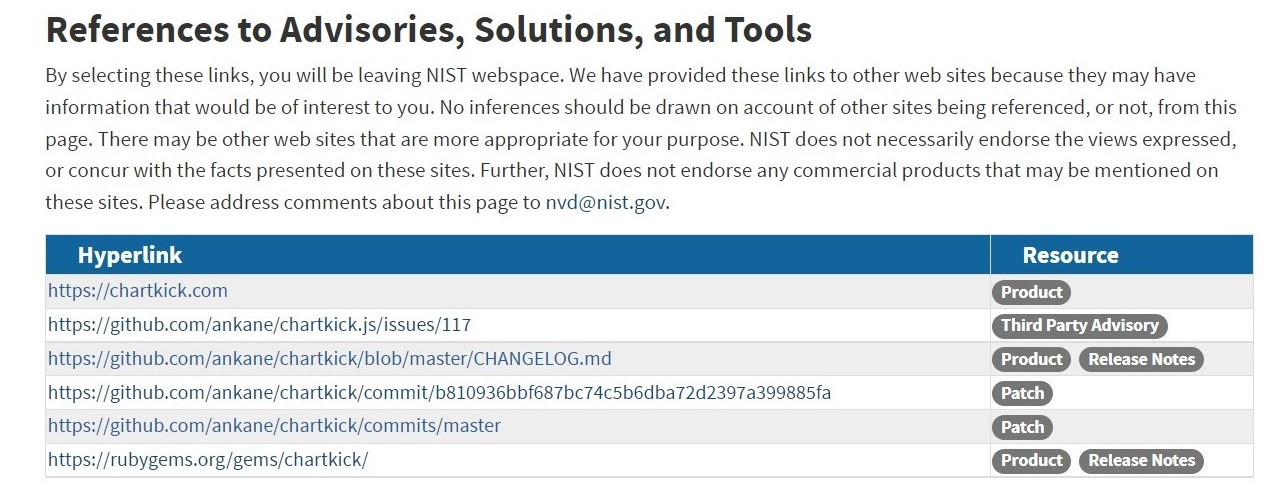
\includegraphics[scale=0.44]{fig/NVD-2019-18841}
    %\vspace{-10pt}
    \caption{NVD平台CVE-2019-18841的引用信息}\label{fig:CVE-2019-18841}
\end{figure*}

\textbf{检索GitHub Commits:}检索GitHub中,检索带有CVE标识符的代码提交\cite{you2017semfuzz,Wang2020empirical}。如图\ref{fig:commitmessage}所示,提交信息(Commit Message)\footnote{https://github.com/apache/tomcat80/commit/2c9d8433bd3247a2856d4b255}为“Fix \url{https://bz.apache.org/bugzilla/show_bug.cgi?id=62343} Make CORS filter defaults more secure. This is the fix for CVE-2018-8014.”,漏洞标识符“CVE-2018-8014”出现在该提交中。以“CVE-2018-8014”为输入,通过检索Github获取该提交,作为漏洞CVE-2018-8014的补丁。
\begin{figure*}[h]
    \centering
    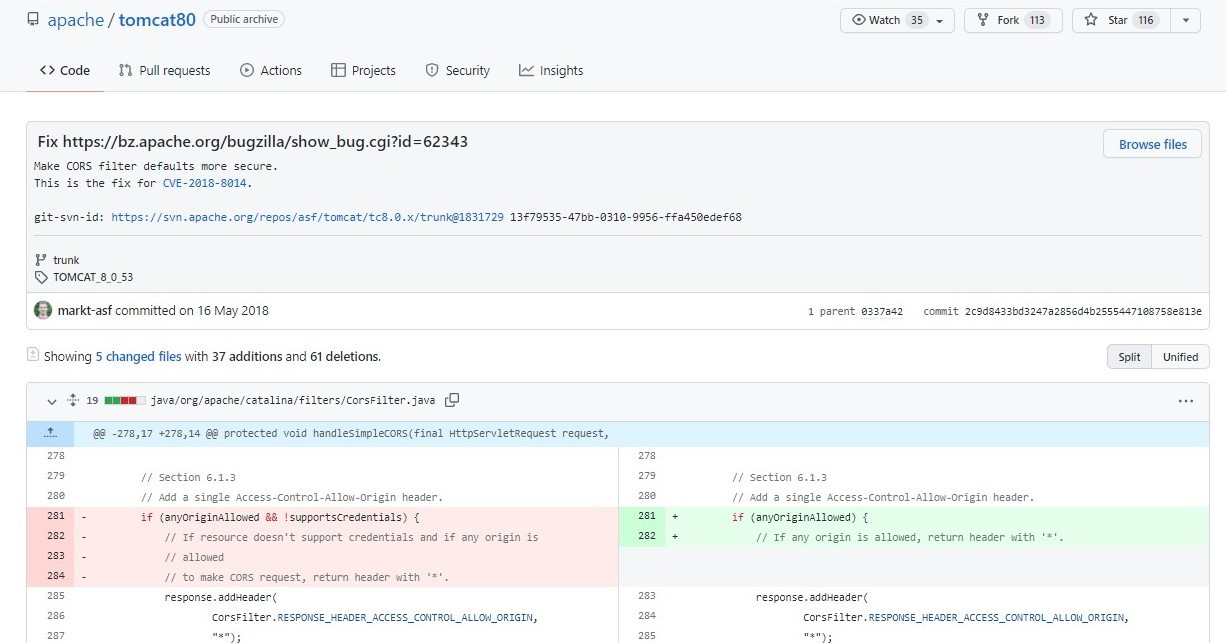
\includegraphics[scale=0.45]{fig/CVE in commit message.jpg}
    %\vspace{-10pt}
    \caption{CVE-2018-8014标识符出现在提交中}\label{fig:commitmessage}
\end{figure*}

\textbf{检索NVD 以及GitHub:}将前两种启发式方法结合为第三种启发式方法,即检索NVD References以及GitHub Commits。

\begin{table*}[h]
    \centering
    % \footnotesize
    \small
    \caption{\tool VS. 已有的基于启发式的方法}\label{table:heuristic}
    %\vspace{-10pt}
    \begin{tabular}{|*{1}{C{4.2em}}|*{1}{C{2.0em}}|*{1}{C{4.9em}}*{3}{C{2.0em}}|*{1}{C{4.9em}}*{3}{C{2.0em}}|}
    % \begin{tabular}{|c|c|cccc|cccc|}
    \noalign{\hrule height 1pt}
    \multirow{2}{*}{映射类型} & \multirow{2}{*}{数量} &  \multicolumn{4}{c|}{检索NVD References} & \multicolumn{4}{c|}{检索GitHub Commits}\\\cline{3-10}
    & & Not Found & Pre. & Rec. & F1 & Not Found & Pre. & Rec. & F1 \\
    \noalign{\hrule height 1pt}
    1:1 (SP) & 567 &	285 (50.3\%) & 0.973 & 0.986 & 0.977 &	472 (83.2\%) & 0.416 & 0.642 & 0.471 	 \\
    1:$i$ (MEP) &195 &	125 (64.1\%) & 0.932 & 0.925 & 0.921 &	162 (83.1\%) & 0.472 & 0.490 & 0.452 	 \\
    1:$n$ (MP) & 101 &	68 (67.3\%) & 0.980 & 0.552 & 0.683 &	73 (72.3\%) & 0.536 & 0.445 & 0.461 	 \\
    1:$n$ (MB) & 372 &	244 (65.6\%) & 0.979 & 0.416 & 0.546 &	246 (66.1\%) & 0.445 & 0.236 & 0.284 	 \\
    1:$n$ (MR) & 60 &	46 (76.7\%) & 1.000 & 0.708 & 0.794 &	37 (61.7\%) & 0.627 & 0.345 & 0.413 	 \\\hline
    Total & 1,295 &	    768 (59.3\%) & 0.970 & 0.805 & 0.842 &	990 (76.4\%) & 0.461 & 0.417 & 0.386 	 \\
    \noalign{\hrule height 1pt}
    \multirow{2}{*}{映射类型} & \multirow{2}{*}{数量} &  \multicolumn{4}{c|}{检索NVD以及GitHub} & \multicolumn{4}{c|}{\tool}\\\cline{3-10}
    & & Not Found & Pre. & Rec. & F1 & Not Found & Pre. & Rec. & F1 \\
    \noalign{\hrule height 1pt}
    1:1 (SP) & 567 &	222 (39.2\%) & 0.839 & 0.930 & 0.864 & 102 (18.0\%) & 0.860 & 0.951 & 0.881 \\
    1:$i$ (MEP) &195 &	104 (53.3\%) & 0.821 & 0.867 & 0.820 & 6 (3.1\%) & 0.886 & 0.918 & 0.888 \\
    1:$n$ (MP) & 101 &	52 (51.5\%) & 0.779 & 0.605 & 0.647  & 20 (19.8\%) & 0.872 & 0.741 & 0.761\\
    1:$n$ (MB) & 372 &	171 (46.0\%) & 0.704 & 0.393 & 0.465 & 23 (6.2\%) & 0.861 & 0.788 & 0.795\\
    1:$n$ (MR) & 60 &	27 (45.0\%) & 0.801 & 0.539 & 0.604  & 4 (6.7\%) & 0.831 & 0.620 & 0.659 \\\hline
    Total & 1,295 &	    576 (44.5\%) & 0.793 & 0.732 & 0.720 & 155 (12.0\%) & 0.864 & 0.864 & 0.837\\
    \noalign{\hrule height 1pt}
    \end{tabular}
\end{table*}

表\ref{table:heuristic}显示了三种启发式方法与\tool 的准确率对比结果。可以发现,对于很大一部分漏洞,三种启发式方法都无法找到其补丁。深度数据集的1295个漏洞中,基于检索NVD References的启发式方法,\tocheck{768(59.3\%)}的漏洞无法找到补丁;基于检索GitHub Commits的启发式方法,\tocheck{990(76.4\%)}的漏洞无法找到补丁;基于检索NVD以及GitHub的启发式方法,\tocheck{576(44.5\%)}的漏洞无法找到补丁;然而,仅\tocheck{155(12.0\%)}漏洞的补丁无法被\tool 找到。

由于NVD References中引用信息都经过人工核对,References中引用信息的置信度比较高,所以基于检索NVD References的启发式方法具有较高的精确率(\tocheck{0.970})。但对于一对多映射关系的CVE,基于检索NVD References的启发式方法召回率就比较低,分别为\tocheck{0.552、0.416和0.708}。这也反映出NVD平台漏洞补丁的不完整情况。基于检索GitHub Commits的启发式方法具有较低的精确率和召回率,分别为\tocheck{0.461}和\tocheck{0.417},而基于检索NVD以及GitHub的启发式方法中和了前两种方法的精确率和召回率分别为\tocheck{0.793}和\tocheck{0.732}。

与基于检索NVD References的启发式方法对比,\tool 的精确率更低,但拥有更高的召回率和相似的F1值;尤其是对于\textit{MP}和\textit{MB}类型的CVE,\tool 的召回率也明显更高。考虑到\tool 找到补丁的漏洞数比第一种启发式方法多出\tocheck{116.3\%},\tool 中轻微的准确率降低是可以接受的。

与基于检索GitHub Commits的启发式方法和基于检索NVD以及GitHub的启发式方法对比,\tool 在精确率、召回率和F1值上全面胜出。\tool 的F1值分别高出了\tocheck{116.8\%}和\tocheck{16.3\%}。

\begin{tcolorbox}[size=title,opacityfill=0.15]
Highlight:与现有的基于启发式的方法相比,\tool 将能找到补丁的漏洞数提高\tocheck{58.6\%}到\tocheck{273.8\%},同时,将F1值提高\tocheck{116.8\%}。
\end{tcolorbox}


\subsection{与商业漏洞数据库对比}
% 考虑到漏洞数据库$DB_A$和$DB_B$并非由工具自动化构建,构建的过程涉及了大量人工工作,并不可知且无法量化,无法进行公平的比较。
% 本节与商业漏洞数据库$DB_A$和$DB_B$进行比较的并非为了证明\tool 或是$DB_A$和$DB_B$的优劣,因为

考虑到漏洞数据库$DB_A$和$DB_B$并非由工具自动化构建,构建的过程涉及了大量人工工作,因此,漏洞数据库$DB_A$和$DB_B$中漏洞信息具有较高的质量。本节将\tool 与数据库$DB_A$和$DB_B$进行对比,可以评估\tool 所达到的准确性水平。如果\tool 可以帮助改进或补充现有的商业漏洞数据库,也能体现\tool 的实用价值。

从表\ref{table:accuracy}和\ref{table:heuristic}可以看出,\tool 能找到补丁的漏洞数比$DB_A$和$DB_B$少了\tocheck{12.0\%},且精确率也分别低了\tocheck{6.4\%}和\tocheck{5.8\%}。这是因为漏洞数据库$DB_A$和$DB_B$构建过程中涉及了安全专家的人工工作,许多补丁由人工收集得来,难以被自动化工具找到。此外,收集的补丁还会经过安全专家验证,因此$DB_A$和$DB_B$也比自动化工具更高的准确率。

此外,\tool 的精确率、召回率和F1值分别为:0.864、0.864和0.837,$DB_A$ 的精确率、召回率和F1值分别为:0.923、0.748和0.793,$DB_B$ 的精确率、召回率和F1值分别为:0.917、0.730和0.771。可以发现\tool 的召回率比$DB_A$和$DB_B$高\tocheck{15.5\%和18.4\%},尤其是对于一对多映射的CVE,\tool 具有更高的召回率;\tool 的F1值也比$DB_A$和$DB_B$高\tocheck{5.5\%和8.6\%}。

这些结果表明,与漏洞数据库$DB_A$和$DB_B$相比,\tool 以较低的精确率和较少未找到补丁的漏洞为代价,拥有更为显着的召回率。这也说明,\tool 可用于补充现有漏洞数据库缺失的漏洞补丁数据。

\begin{tcolorbox}[size=title,opacityfill=0.15]
Highlight:\tool 具有比$DB_A$和$DB_B$高\tocheck{15.5\%和18.4\%}的召回率,以及高\tocheck{5.5\%到8.6\%}的F1值,但同时\tool 牺牲了\tocheck{6.4\%}的精确率和\tocheck{12.0\%}CVE的补丁。
\end{tcolorbox}

\subsection{漏报和误报分析}\label{sec:fpfn}

基于前两小节的实验结果,本小节旨在分析造成\tool 漏报和误报的原因,即\tool 未找到补丁或返回的补丁不正确的情形。

\textbf{漏报分析:} 漏报是指\tool 未能找到补丁或找全补丁,体现在召回率(Recall)小于1,以及Not Found不为0。通过人工分析\tool 未能找到补丁或找全补丁的CVE数据,本小节共总结出\tool 漏报的五个主要原因:
\begin{enumerate}
    \item [(1)] 对于一些年代久远的CVE,NVD、Debian和Red Hat中包含的引用信息比较少,有的引用信息甚至是失效的。这种情况下,\tool 无法构建完整的参考网络。例如,\tool 未能找到补丁的漏洞CVE-2011-1950,该漏洞在NVD\footnote{https://nvd.nist.gov/vuln/detail/CVE-2011-1950}中标记为“补丁(Patch)”和“供应商咨询(Vendor Advisory)”的关键参考链接已经失效,而这个链接中很有可能含有补丁。
    \item [(2)] NVD、Debian和Red Hat平台缺失关键参考链接(例如,问题链接(Issue URL)),\tool 便难以选出正确的补丁。例如,\tool 未能找到补丁的漏洞CVE-2018-14642,其问题报告\footnote{https://issues.redhat.com/browse/UNDERTOW-1430}不包含在任何一个知识源中,人工分析发现,基于此问题报告可以找到该漏洞的补丁\footnote{https://github.com/undertow-io/undertow/commit/c46b7b49c5a561731c84a76ee52244369af1af8a}。
    \item [(3)] 补丁的提交信息不包含CVE标识符,但与CVE描述具有语义相似性,自动化工具难以识别,但可通过人工识别。因此,\tool 的\tocheck{知识源扩增}步骤也未能找到这类型的补丁。例如,漏洞CVE-2019-10077\footnote{https://nvd.nist.gov/vuln/detail/CVE-2019-10077},代码提交\footnote{https://github.com/apache/jspwiki/commit/87c89f0405d6b31fc165358ce5d5bc4536e32a8a}为该漏洞的补丁,但提交信息中未提及CVE标识符,\tool 也未能找到该补丁。
    \item [(4)] GitHub平台用于检索代码提交的REST API仅返回1,000个结果,这会使\tool 在\tocheck{知识源扩增}步骤种错失一些补丁提交。
    \item [(5)] \tool 的补丁精选步骤中,只选择了一个具有最高连通度的补丁节点,其他已包含在参考链接网络中的正确补丁会被遗漏掉,这也造成了漏报。
\end{enumerate}


\textbf{误报分析:}漏报是指\tool 返回的结果非该漏洞的补丁,体现在精确率(Precision)小于1。通过人工分析\tool 返回错误补丁的CVE数据,本小节共总结出\tool 误报的两个主要原因:

\begin{enumerate}
    \item [(1)] 在讨论和解决漏洞时,相关人员也会引用引入漏洞的代码提交。由于\tool 缺乏对参考链接的上下文语义理解,\tool 错误地将其识别为补丁提交。例如,漏洞CVE-2020-5249,引入漏洞的代码提交\footnote{https://github.com/ethereum/go-ethereum/commit/fb9f7261ec51e38eedb454594fc19f00de1a6834}和修复漏洞的代码提交\footnote{https://github.com/ethereum/go-ethereum/commit/83e2761c3a13524bd5d6597ac08994488cf872ef}在同一问题报告(Issue Report)的评论中被引用。
    \item [(2)] 被引用的页面上列出了多对CVE及其问题和补丁。由于\tool 缺乏语义理解,其他CVE的补丁也可能会被\tool 错误地识别。例如,漏洞CVE-2018-15750,其补丁维护在发行说明(Release Note)\footnote{https://docs.saltstack.com/en/latest/topics/releases/2018.3.3.html}中,CVE-2018-15751的发行说明均被NVD、Debian和Red Hat引用。
\end{enumerate}  

\begin{tcolorbox}[size=title,opacityfill=0.15]
Highlight:通过人工分析共总结出\tool 漏报的五个主要原因和误报的两个主要原因,针对这些情形,可进一步提高\tool 的准确性。
\end{tcolorbox}

\section{RQ7:削弱性分析}\label{sec:ablation}

\begin{table*}[h]
    \centering
    \small
    \caption{\tool 削弱性分析结果(1)}\label{table:contribution}
    %\vspace{-10pt}
    \begin{tabular}{|*{1}{C{4.2em}}|*{1}{C{2.0em}}|*{1}{C{4.9em}}*{3}{C{2.0em}}|*{1}{C{4.9em}}*{3}{C{2.0em}}|}
    % \begin{tabular}{|c|c|cccc|cccc|}
    \noalign{\hrule height 1pt}
    \multirow{2}{*}{映射类型} & \multirow{2}{*}{数量} &  \multicolumn{4}{c|}{ \tool } & \multicolumn{4}{c|}{$v_1^1$: \tool w/o NVD} \\\cline{3-10}
    & & Not Found & Pre. & Rec. & F1 & Not Found & Pre. & Rec. & F1  \\
    \noalign{\hrule height 1pt}
    1:1 (SP) & 567 &	102 (18.0\%) & 0.860 & 0.951 & 0.881 &	286 (50.4\%) & 0.820 & 0.936 & 0.846  \\
    1:$i$ (MEP) &195 &	6 (3.1\%) & 0.886 & 0.918 & 0.888 &	    79 (40.5\%) & 0.882 & 0.935 & 0.886 	 \\
    1:$n$ (MP) & 101 &	20 (19.8\%) & 0.872 & 0.741 & 0.761 &	41 (40.6\%) & 0.881 & 0.728 & 0.766 	 \\
    1:$n$ (MB) & 372 &	23 (6.2\%) & 0.861 & 0.788 & 0.795 &	84 (22.6\%) & 0.876 & 0.780 & 0.800 	 \\
    1:$n$ (MR) & 60 &	4 (6.7\%) & 0.831 & 0.620 & 0.659 &	    8 (13.3\%) & 0.848 & 0.551 & 0.624 	 \\\hline
    Total & 1,295 &	    155 (12.0\%) & 0.864 & 0.864 & 0.837 &	498 (38.5\%) & 0.856 & 0.839 & 0.815 	 \\
    \noalign{\hrule height 1pt}

    \multirow{2}{*}{映射类型} & \multirow{2}{*}{数量} &  \multicolumn{4}{c|}{$v_1^2$: \tool w/o Debian} & \multicolumn{4}{c|}{$v_1^3$: \tool w/o Red Hat} \\\cline{3-10}
    & & Not Found & Pre. & Rec. & F1 & Not Found & Pre. & Rec. & F1   \\
    \noalign{\hrule height 1pt}
    1:1 (SP) & 567 &	110 (19.4\%) & 0.847 & 0.943 & 0.869 &	113 (19.9\%) & 0.853 & 0.943 & 0.874 \\
    1:$i$ (MEP) &195 &	8 (4.1\%) & 0.880 & 0.912 & 0.882 &	    7 (3.6\%) & 0.883 & 0.918 & 0.886 \\
    1:$n$ (MP) & 101 &	22 (21.8\%) & 0.851 & 0.716 & 0.739 &	21 (20.8\%) & 0.880 & 0.736 & 0.760 \\
    1:$n$ (MB) & 372 &	28 (7.5\%) & 0.838 & 0.760 & 0.771 &	35 (9.4\%) & 0.844 & 0.761 & 0.767 \\
    1:$n$ (MR) & 60 &	5 (8.3\%) & 0.819 & 0.613 & 0.651 &	    4 (6.7\%) & 0.738 & 0.640 & 0.618 \\\hline
    Total & 1,295 &	    173 (13.4\%) & 0.848 & 0.849 & 0.821 &	180 (13.9\%) & 0.851 & 0.853 & 0.823 \\
    \noalign{\hrule height 1pt}
    
    \multirow{2}{*}{映射类型} & \multirow{2}{*}{数量}  & \multicolumn{4}{c|}{$v_1^4$: \tool w/o GitHub} & \multicolumn{4}{c|}{$v_1^5$: \congyingEdit{\tool w/o Network}} \\\cline{3-10}
    & & Not Found & Pre. & Rec. & F1 & Not Found & Pre. & Rec. & F1  \\
    \noalign{\hrule height 1pt}
    1:1 (SP) & 567 &	149 (26.3\%) & 0.898 & 0.943 & 0.908 &	177 (31.2\%) & 0.910 & 0.972 & 0.925 \\
    1:$i$ (MEP) &195 &	19 (9.7\%) & 0.887 & 0.921 & 0.892 &	78 (40.0\%) & 0.956 & 0.959 & 0.941 \\
    1:$n$ (MP) & 101 &	28 (27.7\%) & 0.873 & 0.690 & 0.726 &	40 (39.6\%) & 0.943 & 0.669 & 0.743 \\
    1:$n$ (MB) & 372 &	39 (10.5\%) & 0.874 & 0.752 & 0.773 &	109 (29.3\%) & 0.908 & 0.575 & 0.659 \\
    1:$n$ (MR) & 60 &	7 (11.7\%) & 0.816 & 0.545 & 0.604 &	10 (16.7\%) & 0.920 & 0.641 & 0.712 \\\hline
    Total & 1,295 &	    242 (18.7\%) & 0.883 & 0.841 & 0.835 &	414 (32.0\%) & 0.918 & 0.812 & 0.823 \\
    \noalign{\hrule height 1pt}
    \end{tabular}
\end{table*}

为了探究\tool 中各个步骤及设计的实际效果及必要性,本小节通过对比\tool 及其削弱部分环节后生成的变体的准确率,以量化分析各步骤及设计的实际效果。

针对步骤一:多源信息网络构建,本小节分别进行了“去除某一知识源”和“去除网络构建步骤”的削弱处理;针对步骤二:补丁节点精选,本小节分别进行了“去除基于连通度和置信度的补丁选择方法”、“去除基于连通度或置信度的补丁选择方法”和“变更基于连通度的方法设置”的削弱处理;针对步骤三:候选补丁扩增,本小节进行了“去除补丁扩增步骤”的削弱处理。表\ref{table:contribution}和\ref{table:contribution-2}展示了削弱性分析的结果,以衡量\tool 中的各步骤和设计对于准确性的贡献度。

\subsection{去除某一知识源} 
在\tool 的步骤一(多源信息网络构建)中,通过分别删除四个知识源NVD、Debian、Red Hat和GitHub中的一个,生成削弱后的变体$v_1^1$、$v_1^2$、$v_1^3$和$v_1^4$。从表\ref{table:contribution}中发现,这四个变体没有找到补丁的CVE数量都是大于\tool 的。在精确率、召回率和F1值相当的情况下,$v_1^1$、$v_1^2$、$v_1^3$和$v_1^4$未找到补丁的漏洞数分别为:498(38.5\%)、173(13.4\%)、180(13.9\%)和242(18.7\%),分别比\tool 多了\tocheck{30.1\%、1.6\%、2.2\%和7.6\%}。这表明,构建更完整的信息网络,也将取得更好的补丁查找结果。\tool 中选取的四个知识源都有助于构建更完整的信息网络,也更有助于为更多的漏洞找到补丁。同时,可以发现,删除知识源NVD和GitHub后未找到补丁的漏洞数增到了498(38.5\%)和242(18.7\%),这也说明知识源NVD和GitHub的贡献度是最高的,效果也是最好的。

\subsection{去除网络构建步骤}
在\tool 的步骤一(多源信息网络构建)中,不以逐层迭代的方式构建信息网络,而是仅仅使用包含在四个知识源公告中的直接引用信息,通过该方式生成削弱后的变体$v_1^5$。具体实现为:在\tool 的步骤一中跳过“引用节点分析”步骤,实验结果为表\ref{table:contribution}中的$v_1^5$。可以发现,$v_1^5$没有找到补丁的CVE数量增加到了414(32.0\%)。在数值上,$v_1^5$找到补丁的漏洞数比\tool 少了\tocheck{22.7\%},但同时精确率却高出了\tocheck{6.3\%},召回率低了\tocheck{6.0\%},F1值较为相似。这些结果表明,补丁并不总是在NVD、Debian和Red Hat中被直接引用,而是可能隐藏在多层引用信息之中;同时说明,本文构建的信息网络有助于用户找到隐藏的补丁,但需要以小幅的精确率降低为代价。


\begin{table*}[h]
    \centering
    \small
    \caption{\tool 削弱性分析结果(2)}\label{table:contribution-2}
    %\vspace{-10pt}
    \begin{tabular}{|*{1}{C{4.2em}}|*{1}{C{2.0em}}|*{1}{C{4.9em}}*{3}{C{2.0em}}|*{1}{C{4.9em}}*{3}{C{2.0em}}|}
    % \begin{tabular}{|c|c|cccc|cccc|}
    \noalign{\hrule height 1pt}
    
    \multirow{2}{*}{映射类型} & \multirow{2}{*}{数量} &  \multicolumn{4}{c|}{$v_2^1$: \congyingEdit{\tool w/o Selection}} & \multicolumn{4}{c|}{$v_2^2$: \tool w/o Connectivity} \\\cline{3-10}
    & & Not Found & Pre. & Rec. & F1 & Not Found & Pre. & Rec. & F1 \\
    \noalign{\hrule height 1pt}
    1:1 (SP) & 567 &	102 (18.0\%) & 0.632 & 0.961 & 0.680 &	245 (43.2\%) & 0.892 & 0.978 & 0.913  \\
    1:$i$ (MEP) &195 &	6 (3.1\%) & 0.622 & 0.976 & 0.682 &	    111 (56.9\%) & 0.929 & 0.939 & 0.915  \\
    1:$n$ (MP) & 101 &	20 (19.8\%) & 0.615 & 0.933 & 0.656 &	56 (55.4\%) & 0.953 & 0.685 & 0.764  \\
    1:$n$ (MB) & 372 &	23 (6.2\%) & 0.616 & 0.903 & 0.657 &	191 (51.3\%) & 0.927 & 0.787 & 0.821  \\
    1:$n$ (MR) & 60 &	4 (6.7\%) & 0.368 & 0.891 & 0.394 &	    27 (45.0\%) & 0.885 & 0.722 & 0.772  \\\hline
    Total & 1,295 &	155 (12.0\%) & 0.611 & 0.940 & 0.658 &	    630 (48.6\%) & 0.910 & 0.889 & 0.871  \\
    \noalign{\hrule height 1pt}

    \multirow{2}{*}{映射类型} & \multirow{2}{*}{数量} & \multicolumn{4}{c|}{$v_2^3$: \tool w/o Confidence} &  \multicolumn{4}{c|}{$v_2^4$: \tool with Path Length} \\\cline{3-10}
    & & Not Found & Pre. & Rec. & F1 & Not Found & Pre. & Rec. & F1 \\
    \noalign{\hrule height 1pt}
    1:1 (SP) & 567 &	102 (18.0\%) & 0.860 & 0.942 & 0.879  & 102 (18.0\%) & 0.833 & 0.957 & 0.859\\
    1:$i$ (MEP) &195 &	6 (3.1\%) & 0.888 & 0.913 & 0.889 &     6 (3.1\%) & 0.848 & 0.945 & 0.867 \\
    1:$n$ (MP) & 101 &	20 (19.8\%) & 0.880 & 0.722 & 0.751 &   20 (19.8\%) & 0.849 & 0.760 & 0.742\\
    1:$n$ (MB) & 372 &	23 (6.2\%) & 0.871 & 0.765 & 0.784 &    23 (6.2\%) & 0.830 & 0.798 & 0.770\\
    1:$n$ (MR) & 60 &	4 (6.7\%) & 0.849 & 0.462 & 0.550 &     4 (6.7\%) & 0.652 & 0.747 & 0.590 \\\hline
    Total & 1,295 &	    155 (12.0\%) & 0.869 & 0.844 & 0.826 &  155 (12.0\%) & 0.827 & 0.882 & 0.812 \\
    \noalign{\hrule height 1pt}

    
    \multirow{2}{*}{映射类型} & \multirow{2}{*}{数量} &   \multicolumn{4}{c|}{$v_2^5$: \tool with Path Number} & \multicolumn{4}{c|}{$v_3$: \tool w/o Expansion} \\\cline{3-10}
    & & Not Found & Pre. & Rec. & F1 & Not Found & Pre. & Rec. & F1 \\
    \noalign{\hrule height 1pt}
    1:1 (SP) & 567 &	102 (18.0\%) & 0.805 & 0.951 & 0.837 &  102 (18.0\%) & 0.871 & 0.948 & 0.889\\
    1:$i$ (MEP) &195 &	6 (3.1\%) & 0.849 & 0.920 & 0.858 &     6 (3.1\%) & 0.910 & 0.914 & 0.902\\
    1:$n$ (MP) & 101 &	20 (19.8\%) & 0.801 & 0.756 & 0.726 &   20 (19.8\%) & 0.873 & 0.696 & 0.732\\
    1:$n$ (MB) & 372 &	23 (6.2\%) & 0.833 & 0.811 & 0.791 &    23 (6.2\%) & 0.860 & 0.506 & 0.590\\
    1:$n$ (MR) & 60 &	4 (6.7\%) & 0.789 & 0.630 & 0.644 &     4 (6.7\%) & 0.847 & 0.567 & 0.629\\\hline
    Total & 1,295 &	    155 (12.0\%) & 0.819 & 0.873 & 0.809 &  155 (12.0\%) & 0.873 & 0.771 & 0.776\\
    \noalign{\hrule height 1pt}
    \end{tabular}
\end{table*}

\subsection{去除补丁精选步骤}
\textbf{去除基于连通度和置信度的补丁选择方法:}
在\tool 的步骤二(补丁节点精选)中,并非选择具有高置信度和连通度的补丁,而是选择网络中的所有补丁。生成的变体为表\ref{table:contribution}中的$v_2^1$,可以看到该变体显着提高了\tool 的召回率,由0.864提高到了0.940多了\tocheck{8.8\%},尤其是对于一对多映射类型的CVE。但同时精确率大幅下降\tocheck{29.3\%},由0.864降到了0.611;F1值也大幅下降了\tocheck{21.4\%},由0.837降到了0.658。该结果表明,参考链接网络中确实包含了大部分漏洞的正确补丁,且基于启发式的补丁选择方法有助于实现精确率和召回之间的平衡。

\textbf{去除基于连通度或置信度的补丁选择方法:}
在\tool 的步骤二(补丁节点精选)中,并非选择具有高置信度和连通度的补丁,而是采用两个启发式方法之一,即选择具有高置信度或连通度的补丁,生成两个变体$v_2^2$和$v_2^3$。

在不使用基于连通度的启发式方法时,$v_2^2$找到补丁的漏洞数比\tool 少了\tocheck{41.7\%},但同时精确率提升了\tocheck{5.3\%},召回率提高了\tocheck{2.9\%},F1值提高了\tocheck{4.1\%}。这些结果表明,基于连通度的启发式有助于为更多CVE找到补丁,但同时也会引入少部分噪声。
在不使用基于置信度的启发式方法时,$v_2^3$的召回率和F1值会略有下降,分别由0.864和0.837降到了0.844和0.826;尤其是对于\textit{MR}类型的CVE,影响更为明显,召回率由0.620下降到0.462。

这些结果表明,基于置信度的启发式方法有助于在所有评估标准(Not Found、Precision、Recall和F1-Score)之间实现平衡的准确性。

\textbf{变更基于连通度的方法设置:}
在\tool 的步骤二(补丁节点精选)基于连通度的方法中,通过仅考虑路径长度(即选择到根节点的路径最短的补丁)和仅考虑路径数量(即选择具有最多路径数的补丁)来削弱基于连通度的启发式方法,分别生成了变体$v_2^4$和$v_2^5$。

$v_2^4$和$v_2^5$的精确率分别比\tool 低了\tocheck{4.3\%}和\tocheck{5.2\%},召回率分别高了\tocheck{2.1\%}和\tocheck{1.0\%},F1值分别降低了\tocheck{3.0\%}和\tocheck{3.3\%}。这些结果表明,基于连通度的启发式方法中所设计的补丁节点到根节点的路径长度和路径数都有助于提高\tool 的准确率。

\subsection{去除补丁扩增步骤}
去除\tool 的步骤三(候选补丁扩增)后,生成变体$v_3$。可以发现,$v_3$的召回率为0.771,比\tool 的召回率下降了\tocheck{10.8\%};$v_3$的F1值为0.776,比\tool 的F1值下降了\tocheck{7.3\%}。尤其是对于一对多映射类型的CVE,召回率和F1值下降更为显著。这些结果表明,补丁扩增步骤有助于\tool 更完整地为漏洞找到多个补丁。

\begin{tcolorbox}[size=title,opacityfill=0.15]
Highlight:\tool 中的知识源、网络构建、补丁选择和补丁扩增步骤及其中的设计都具有一定的效果和必要性,都对\tool  补丁查找的准确性做出了贡献。
\end{tcolorbox}

\section{RQ8:敏感度分析}\label{sec:sensitivity}
% \begin{figure*}[h]
%     \centering
%     \begin{subfigure}[b]{0.45\textwidth}
%     \centering
%     \includegraphics[scale=0.55]{fig/rq8-sensitivity-depth.pdf}
%     %\vspace{-5pt}
%     \caption{网络深度限制}\label{fig:depth}
%     \end{subfigure}
%     \begin{subfigure}[b]{0.45\textwidth}
%     \centering
%     \includegraphics[scale=0.55]{fig/rq8-sensitivity-span.pdf}
%     %\vspace{-5pt}
%     \caption{提交时间跨度}\label{fig:span}
%     \end{subfigure}
%     %\vspace{-20pt}
%     \caption{网络深度限制和提交时间跨度的敏感性分析结果}\label{fig:sensitivity}
% \end{figure*}

本小节为探究\tool 的准确性对\tool 中参数的敏感性,\tool 中有两个可配置的参数,分别是:\tool 步骤一网络构建时网络深度限制的设置,以及步骤三补丁扩增时的相关代码提交时间跨度的设定。

验证\textbf{RQ6 准确性验证}、\textbf{RQ7 削弱性分析}、\textbf{RQ9 通用性分析}和\textbf{RQ10 实用性能分析}时,网络深度限制默认设置为\textbf{5}层,代码提交时间跨度默认设置为\textbf{30}天。为了评估\tool 对这两个参数的敏感性,该小节将分别固定两个参数中的一个为默认设置,改变另一个参数的设置,并在深度数据集上重新运行\tool 。网络深度限制具体设置为3、4、5和6层,提交时间跨度具体设置为0、10、20、30、40、50和60天。
\begin{figure*}[h]
    \centering
    \includegraphics[scale=1.0]{fig/rq8-sensitivity-depth.pdf}
    %\vspace{-5pt}
    \caption{网络深度限制(层数)敏感性分析结果}\label{fig:depth}
\end{figure*}

\begin{figure*}[h]
    \centering
    \includegraphics[scale=1.0]{fig/rq8-sensitivity-span.pdf}
    %\vspace{-20pt}
    \caption{提交时间跨度的敏感性分析结果}\label{fig:span}
\end{figure*}


图\ref{fig:depth}和\ref{fig:span}分别显示了两个参数对\tool 准确性的影响,其中横坐标$x$-axis表示参数的取值,纵坐标$y$-axis表示\tool 的精确率。总体来看,随着网络层数的增加,网络中将包含更多补丁。此时,\tool 未发现补丁的漏洞数量在降低,精确率也在降低,而召回率和F1值先增加后降低。
基于图\ref{fig:depth}中数据,可以认为网络深度限制设置为5层时,\tool 效果最优。

随着代码提交时间跨度的增加,\tool 会搜索到更广的代码提交。\tool 的精确率也会降低,召回率会提高,F1值先上升后下降。其中,\tool 未找到补丁的漏洞数量并不改变,所以没有在图\ref{fig:span}中显示。基于图\ref{fig:span}中数据,可以认为提交时间跨度设置为30天时,\tool 效果最优。

\begin{tcolorbox}[size=title,opacityfill=0.15]
Highlight:总的来说,\tool 的精确率对两个可配置参数的变化不是很敏感。
\end{tcolorbox}

\section{RQ9:通用性分析}\label{sec:generality}

% \begin{table*}[h]
%     \centering
%     \footnotesize
%     \caption{Generality of \tool over Two Additional Datasets}\label{table:generality}
%     %\vspace{-10pt}
%     % \begin{tabular}{|c|*{1}{C{5.1em}}|*{3}{C{2.6em}}|*{1}{C{5.1em}}*{3}{C{2.5em}}|*{1}{C{5.1em}}*{3}{C{2.5em}}|}
%     \begin{tabular}{|c|c|ccc|cccc|cccc|}   
%     \noalign{\hrule height 1pt}
%     \multirow{2}{*}{Dataset} & \multirow{2}{*}{Number} &  \multicolumn{3}{c|}{\tool} & \multicolumn{4}{c|}{$DB_A$} & \multicolumn{4}{c|}{$DB_B$} \\\cline{3-13}
%     & & Pre. & Rec. & F1 & Not Found & Pre. & Rec. & F1  & Not Found &  Pre. & Rec. & F1 \\
%     \noalign{\hrule height 1pt}
%     First Dataset & 91 & 0.823 & 0.845 & 0.784  & 29 (31.8\%) &  0.935 & 0.827 & 0.858  & 62 (68.1\%) & 0.885 & 0.664 & 0.725\\\hline
%     Second Dataset & 89 & 0.888 & 0.899 & 0.867 & --& -- & -- & -- & -- & -- & -- & -- \\\hline
%     \noalign{\hrule height 1pt}
%     \end{tabular}
% \end{table*}

为了评估\tool 在更大范围的开源软件漏洞上表现,即\tool 的通用性,本节还另外构建了两个更大的漏洞数据集。第一个数据集为:漏洞数据库$DB_A$和$DB_B$中只有一个数据库提供补丁的CVE(图\ref{fig:rq1-cves-with-patches}中的橙色和蓝色部分),共有\tocheck{3,185}个CVE。第二个数据集为:两个漏洞数据库都没有提供补丁的CVE(图\ref{fig:intersection}),共有\tocheck{5,468}个CVE。

对于第一个数据集中的\tocheck{3,185}个CVE,\tool 找到了\tocheck{2,155(67.7\%)}漏洞的补丁,而两个漏洞数据库$DB_A$和$DB_B$仅分别提供了\tocheck{2,190(68.8\%)}和\tocheck{995(31.2\%)}漏洞的补丁。在\tool 找到补丁的\tocheck{2,155}个漏洞中,$DB_A$和$DB_B$仅提供了其中的\tocheck{1,455}和\tocheck{700}个漏洞的补丁。对于第二个数据集中的\tocheck{5,468}个CVE,\tool 找到了\tocheck{2,816(51.5\%)}漏洞的补丁,而两个漏洞数据库$DB_A$和$DB_B$没有提供补丁。

\begin{table*}[h]
    \centering
    \small
    \caption{\tool 通用性分析结果}\label{table:generality}
    %\vspace{-10pt}
    % \begin{tabular}{|c|*{1}{C{5.3em}}|*{3}{C{2.4em}}|*{1}{C{5.3em}}|*{3}{C{2.4em}}|}
    \begin{tabular}{|c|c|ccc|c|ccc|}
    \noalign{\hrule height 1pt}
    \multirow{2}{*}{验证对象} &  \multicolumn{4}{c|}{{数据集一 (91个CVE)}} & \multicolumn{4}{c|}{数据集二(89个CVE)} \\\cline{2-9}
    & Not Found & Pre. & Rec. & F1 & Not Found & Pre. & Rec. & F1 \\
    \noalign{\hrule height 1pt}
    \tool  & 0 (0.0\%) & 0.823 & 0.845 & 0.784      & 0 (0.0\%) & 0.888 & 0.899 & 0.867       \\\hline
    $DB_A$  & 29 (31.8\%) &  0.935 & 0.827 & 0.858      & 89 (100.0\%) & -- & -- & --        \\\hline
    $DB_B$  & 62 (68.1\%) & 0.885 & 0.664 & 0.725      & 089(100.0\%) & -- & -- & --        \\\hline
    \noalign{\hrule height 1pt}
    \end{tabular}
\end{table*}

此外,本节还从\tool 在第一个和第二个数据集上能找到补丁的CVE中分别采样了\tocheck{100}个,并采用“数据准备”(见章节\ref{sec:preparation})中同样的方式手动找到它们的补丁以评估\tool 的准确性,表\ref{table:generality}为评估结果。由于公开的信息有限,人工分析的两份数据集中分别有\tocheck{9}和\tocheck{11}个CVE不能确定其补丁。

在第一个数据集取样的\tocheck{91}个CVE中,\tool 的F1值为\tocheck{0.784},$DB_A$的F1值较高为0.858,$DB_B$的F1值较低为0.725。与小节\ref{sec:accuracy-evaluation}中的结果类似,漏洞数据库$DB_A$和$DB_B$都拥有更高的精确率(0.935和0.885),但召回率也更低(0.827和0.664)。在第二个数据集取样的\tocheck{89}CVE中,$DB_A$和$DB_B$中没有任何漏洞的补丁,而\tool 可取得达到\tocheck{0.867}的F1值,0.888的精确率和0.899的召回率。

这些结果表明,即使对于更大范围的开源软件漏洞,\tool 的准确率也基本稳定,对于开源软件漏洞的补丁定位,\tool 具有较好的通用性。尤其在第二个数据集上的结果,漏洞数据库$DB_A$和$DB_B$没有提供补丁时,\tool 仍可以找到大量漏洞的补丁,可以极大地补充或增强现有的商业漏洞数据库


\begin{tcolorbox}[size=title,opacityfill=0.15]
Highlight:\tool 在两个更大的开源漏洞数据集上可查找到\tocheck{67.7\%}和\tocheck{51.5\%}CVE的补丁,通过采样评估,精确率分别为\tocheck{0.823}和\tocheck{0.888},召回率分别为\tocheck{0.845}和\tocheck{0.899},体现出\tool 在查找开源漏洞补丁方面具有较好的通用性。
%\congyingEdit{此外,它还表明\tool可以帮助补充现有的漏洞数据库。}
\end{tcolorbox}

\section{RQ10: 实用性分析}\label{sec:usefulness}
本小节旨在评估\tool 在实际使用中的实用性。在实际使用中,为了确保补丁的准确性,安全专家即使使用了较准确的自动工具查找到补丁,他们仍然需要对补丁进行多次确认。为了评估\tool 在这种使用场景中的实用性,本文作者邀请了10名参与者进行了一项用户研究,参与者将分别在有和没有\tool 的辅助下找到10个CVE的补丁。

本文作者从国内外多所大学和科技公司的安全实验室中共招募了10名参与者,他们中有软件安全方向的博士后、博士生、硕士研究人员以及工程师。该用户研究从深度数据集中随机选择了10个CVE作为实验任务,其中,2个CVE属于\textit{SP}类型,3个CVE属于\textit{MEP}类型,1个CVE属于\textit{MP}类型,4个CVE属于\textit{MB}类型。为了公平比较,该用户研究将参与者平均分为A、B两组。A组人员需要在不使用\tool 的情况下完成前五项任务,并使用\tool 完成剩余的任务。反之,B组人员需要在使用\tool 的情况下完成前5个任务,并在不使用\tool 完成剩余的任务。

% \begin{table*}[h]
%     \centering
%     \footnotesize
%     \caption{用户研究中10个任务的用时和准确率对比结果}\label{table:usefulness}
%     %\vspace{-10pt}
%     \begin{tabular}{|c|*{1}{C{5.3em}}|*{3}{C{2.4em}}|*{1}{C{5.3em}}|*{3}{C{2.4em}}|*{1}{C{5.3em}}|*{3}{C{2.4em}}|}
%     \noalign{\hrule height 1pt}
%     \multirow{2}{*}{Approach} &  \multicolumn{4}{c|}{{All 10 Tasks}} & \multicolumn{4}{c|}{5 Single-Patch Tasks} & \multicolumn{4}{c|}{5 Multiple-Patches Tasks} \\\cline{2-13}
%     & Time (mins) & Pre. & Rec. & F1 & Time (mins) & Pre. & Rec. & F1 & Time (mins) &  Pre. & Rec. & F1 \\
%     \noalign{\hrule height 1pt}
%     w/o \tool & 5.66 & 0.880 & 0.677 & 0.765      & 5.60 & 0.960 & 0.960 & 0.960        & 5.72 & 0.800 & 0.393 & 0.527 \\\hline
%     with \tool  & 4.66 & 0.983 & 0.920 & 0.951      & 3.84 & 1.000 & 1.000 & 1.000        & 5.48 & 0.967 & 0.840 & 0.899 \\\hline
%     \noalign{\hrule height 1pt}
%     \end{tabular}
% \end{table*}

\begin{table*}[h]
    \centering
    \small
    \caption{用户研究中10个任务的用时和准确率}\label{table:usefulness}
    %\vspace{-10pt}
    % \begin{tabular}{|c|*{1}{C{5.3em}}|*{3}{C{2.4em}}|*{1}{C{5.3em}}|*{3}{C{2.4em}}|}
    \begin{tabular}{|c|c|ccc|c|ccc|}
    \noalign{\hrule height 1pt}
    \multirow{2}{*}{任务} &  \multicolumn{4}{c|}{{w/o \tool}} & \multicolumn{4}{c|}{with \tool} \\\cline{2-9}
    & 用时 & Pre. & Rec. & F1 & 用时 & Pre. & Rec. & F1 \\
    \noalign{\hrule height 1pt}
    全部10个任务  & 5.66 mins & 0.880 & 0.677 & 0.765      & 4.66 mins& 0.983 & 0.920 & 0.951        \\\hline
    5单补丁任务  & 5.60 mins & 0.960 & 0.960 & 0.960      & 3.84 mins& 1.000 & 1.000 & 1.000        \\\hline
    5多补丁任务  & 5.72 mins & 0.800 & 0.393 & 0.527      & 5.48 mins& 0.967 & 0.840 & 0.899        \\\hline
    \noalign{\hrule height 1pt}
    \end{tabular}
\end{table*}


表\ref{table:usefulness}显示了10个任务的平均时间消耗和补丁的准确性。本节将属于\textit{SP}和\textit{MEP}的5个CVE归类为\textit{单补丁}任务,将属于\textit{MP}和\textit{MB}的5个CVE归类为\textit{多补丁}任务。

总体而言,对于全部10个任务,在\tool 的帮助下,参与者完成每个任务的用时较少(平均4.66分钟),比在没有使用\tool 时少用了\tocheck{17.7\%}时间;在\tool 的帮助下,补丁的精确率为0.983,召回率为0.920,F1值为0.951,对比没有\tool 时,分别提高了\tocheck{11.7\%},\tocheck{35.9\%}和\tocheck{24.3\%}。

对于5个\textit{单补丁}任务,在\tool 的帮助下,参与者用时显然更短,但对于5个\textit{多补丁}任务,参与者用时基本持平。这是因为\tool 为\textit{多补丁}任务返回的信息网络和补丁比\textit{单补丁}任务的更复杂,参与者需要花费更多的时间以理解信息网络,并验证其中的补丁。此外,在\tool 的帮助下,对于5个\textit{多补丁}任务的准确度的高也较为显着,但对于5个\textit{单补丁}任务则并不显着。这是因为,\textit{单补丁}任务相比\textit{多补丁}任务较为简单,参与者无需tool 的帮助即可完成补丁查找。这也表明,\tool 对于具有多个补丁的开源漏洞作用更为明显。

本文作者还采访了每位参与者,以获取参与者对\tool 评价及使用感受。总体来说,参与者都认为漏洞的信息网络具有较高的价值,因为它囊括了来自多个知识源的信息,其中,不同类型的节点和关系有助于人工定位和验证补丁。一家来自科技公司的安全工程师评论:\textit{``信息网络作为一个证据链,有助于定位和验证补丁"}。此外,参与者还建议:\tool 可以添加更多的知识源,并提供更多关于补丁节点的信息,如:提交消息和代码差异等,这些信息有助于人工审查补丁。

\begin{tcolorbox}[size=title,opacityfill=0.15]
Highlight:在实际使用中,\tool 有助于用户更准确、更快速地查找到补丁。
\end{tcolorbox}

\section{讨论}

基于上文实验验证的结果,以及\tool 的设计,本节将主要讨论\tool 存在的短板和潜在的价值。
\subsection{\tool 的局限性}
\tool 以CVE ID作为输入,因此该方法不适用于没有CVE ID的开源漏洞(即不在CVE平台中的开源漏洞),比如一些秘密修补的漏洞并没有收录在CVE平台中,也没有CVE ID。一种可能的解决方案是将Advisory-ID作为\tool 的输入。

\tool 仅仅包含Debian和Red Hat两个次级知识源,也因此会遗漏在其他知识源中出现的补丁。但\tool 具有较好的可扩展性,它可以灵活地扩增其他知识源(例如,SecurityFocus\footnote{https://www.securityfocus.com})。

此外,小节(见章节\ref{sec:fpfn})中也阐述了造成\tool 漏报和误报的诸多原因。

\subsection{\tool 的价值}
\tool 将会有益于软件安全领域相关的社区、学术界和工业界的研究人员。对于安全社区而言,\tool 可以发现缺少补丁的漏洞,并向NVD管理员报告该情况,以提高CVE的信息质量并加速CVE条目的更新,使得NVD平台的用户受益。对于学术界而言,\tool 可以为大规模数据驱动的安全分析工作(例如,基于学习的漏洞检测\cite{li2018vuldeepecker,zhou2019devign})和经验研究工作提供基础的补丁数据。%它还可以帮助通过分析漏洞补丁以确定受影响组件的工作\cite{dong2019towards}。
对于工业界来说,\tool 可以帮助安全工程师提高商业漏洞数据库的补丁覆盖率和准确性,从而提高软件成分分析的准确性。值得一提的是,\tool 已经部署到一家高科技公司。但是,由于保密协议,本文不便分享相关数据。
% \chapter{相关工作}
\chapter{总结与展望}

本章节总结与展望。

\section{本文总结}

本文总结本文总结本文总结本文总结本文总结本文总结本文总结本文总结

\section{未来展望}

未来展望未来展望未来展望未来展望未来展望未来展望未来展望未来展望

% 后置部分包含参考文献、声明页(自动生成)等
\backmatter

\printbibliography                    % 参考文献列表
\chapter{致谢}  % 致谢
% \chapter{初审意见修改说明}

% \begin{enumerate}[]
%   \item \strong{方法叙述上,应该多加论述为什么,而不仅是罗列过程。}\\
%   在第三章描述各个方案前补充了这么做的原因。
%   \item \strong{写作需要进一步全文通读理顺。}\\
%   通读了全文,统一了一些名词、修正了语法错误、改进了一些措辞表达和语序。
% \end{enumerate}           % 评审意见修改

\end{document}
